\documentclass[a4paper,12pt]{article}

\usepackage{graphicx}
\usepackage{caption}
\usepackage{subcaption}
\usepackage{algorithm}
\usepackage{algorithmic}
\usepackage{amsmath}


\begin{document}

\title{FLIP Water Simulation using Multigrid Pressure Solver}
\author{Per Karlsson}
\date{February 2014}
\maketitle

\begin{abstract}
This thesis involves an evaluation of the multigrid method for solving systems of differential equations in hybrid particle-grid fluid simulations. The work in this thesis is focused on inviscid incompressible liquid and water simulations and the method of choice is Fluid Implicit Particle, FLIP. All equations and algorithms are presented in a two-dimensional domain but none of the solutions are restricted to the two dimensions and it is straightforward to handle them in three dimensions.
\newline
\newline
The implementation in this thesis is based on the Navier-Stokes fluid equations and the Level Set methods for surface tracking. The fundamentals of these are explained in the first chapters and solutions to the equations are presented later on. This report tells you how to store explicit particle velocites in an implicit grid and how to integrate particle velocities from a grid. A large portion of this thesis explains the multigrid method and how to implement one for solving the pressure equations needed in a fluid simulation.
\newline
\newline
The results of the multigrid pressure solver in this thesis shows that the method is good enough for non real-time simulations in computer graphics. To test correctness, a comparison between multigrid and the traditional preconditioned conjugate gradient method showed similar results.

\end{abstract}


\tableofcontents
\setcounter{tocdepth}{2}

\newpage
\section{Introduction}
In general, computer graphics tries to come up with methods to represent what we see and interpret with our eyes, where the main goal has always been to produce an image in the end that looks reasonable. There are two restrictions, time and accuracy. In most cases, we do not have unlimited time to produce each image, especially not in animation where there are 24 images per second that have to be constructed. The other limitation is accuracy. Some problems we do not know how to model and some problems we do not know how to solve precisely. Simplifications are accepted as long as the end result looks convincing. 
\newline
\newline
In the field of animation, we care about how objects move in space and how they deform over time. Many problems can be solved by simply moving objects in space manually, often referred to as hand-animating. A common technique for animating characters in the visual effects and video games industry is to only animated a simplified skeleton and then weight geometry to different parts of the skeleton. This is fine for a characters main movement. However, for more complex things on characters, like hair and cloth, simple hand-animated approaches do not work anymore. There are too many hair strands or wrinkles on the cloth to control them all manually. Even if we would attempt to, it is very likely that the motion would look unreal. For more complex phenomena we need to simulate the objects and their geometry for a convincing motion.
\newline
\newline
This report focus on simulation of interesting water effects. Liquid fluids have, unlike their gas state, a surface defining their volume. The surface has a lot of degrees of freedom and can take any shape. To make it even more complex, it also changes topology over time which makes it hard to write surface tracking implementations. The other challenging part of fluid simulation is to define how the velocity in the fluid is changing over time where each little part of the fluid can have a velocity completely different from its neighbors. 

\subsection{Background}

There have mainly been two different traditional ways of trying to solve the fluid equations, the Lagrangian viewpoint and the Eulerian viewpoint. The Lagrangian approach treats continuum like a particle system where each point in the fluid is labeled as a particle with a position and velocity. The Smoothed Particle Hydrodynamics\cite{sph}, SPH, was introduced to computational fluid dynamics and animation by Desbrun and Cani\cite{desbrun}. The big advantage of SPH is that the advection step does not suffer from any numerical smoothing and act directly on the particles. It gets trickier to approximate spatial derivates since it completely depends on where and how many particles there are nearby. This can lead to instability in the simulation. Eulerian methods are grid based and instead of tracking a part of the fluid as it moves, they focus on tracking a fixed point in space and check how the fluid quantites at that point are changing over time. Foster and Metaxas\cite{metaxas} introduced the first 3D grid based water simulation. One problem in the beginning of grid based solutions was that it tended to blow up eventually and it was not stable for long simulations. J.Stam\cite{stam} added a semi-langrangian advection to the grid based methods and made it unconditionally stable which allowed larger timesteps than before. To track surfaces, signed distance fields and level sets were used. Fedkiw and Foster\cite{fosterfed} introduced a way to combine particles and level set for better surface tracking and therefore have less volume loss in the simulation. Unlike the Lagrangian approach, approximating a spatial derivate is a lot easier on a grid where one can just look at the difference between neighboring cells. Grid methods have many steps that requires interpolation, which tend to smooth out interesting high frequency motion in the fluid.
\newline
\newline
Both the Lagrangian and Eulerian have their advantages and disadvantges. Zhou and Bridson\cite{zhu} came up with a way of combining them to have a stable pressure solving step on a grid and a Lagrangian advection step. This method is usually called FLIP. Zhou and Bridson used a preconditioned conjugate gradient solver for solving the pressure equations. In this report we are going to use the Multigrid approach instead, inspired by Mueller\cite{mueller}.

\subsection{Purpose}

%\subsection{Structure}


\newpage
\section{Fundamentals}
This chapter will explain the major concepts that one needs to know about before attempting to implement a FLIP fluid solver. It will explain the theory behind the fluid equations and how to improve accuracy when dealing with discretization of differential equations. An overview of the overall FLIP algorithm is presented at the end of the chapter.

\subsection{Navier-Stokes equations}

Most fluid research in computer graphics is based on the famous incompressible Navier-Stokes equations. The equations can be written in many different ways but usually it can be seen as

\begin{equation}
du + u* + p = g
\end{equation}

\begin{equation}
\nabla \cdot \vec{u} = 0
\end {equation}

In Equation 1, $\vec{u}$ is the velocity field of the fluid, $\rho$ is the pressure, $\vec{f}$ represent all the external forces acting on the fluid (such as gravity) and $v$ is the viscosity constant. This report empashizes on liquid simulations and in particular, water simulations. Water is, by nature, a very non viscious fluid. This means that the term in the Navier-Stokes equations that involves viscousity is relative less important and can be neglected. If we drop the viscousity term in Equation 1, we get

\begin{equation}
du + u* + p = g
\end{equation}

which is also known as the Euler fluid equations. The fluid we are now trying to simulate is called an inviscid fluid. Even though we have removed the viscousity from the equations, it still means that the fluid we simulate can look viscious. This is because of the numerical methods and the errors they introduce. An important reason we prefer the hybrid Lagrangian/Eulerian method in this report is so we can avoid a lot of the numerical dissipation shown in pure grid based solutions that involes a lot of linear interpolation. 
\newline

At first, Equation 3 might look a bit complicated. To get a better understanding of the different terms, let us start with a simple example where the scalar quantity $c$ is depending on where in space and time it is evaluated. $c$ is said to be a function of spatial coordinates $\vec{x}$ and time $t$, $c(t,\vec{x})$. To find out how much $c$ is changing at coordinate $\vec{x}$, we take the temporal derivate of $c$.

\begin{equation}
dc(t,\vec{x}) = dc + \nabla q \cdot d\vec{x}
\end{equation}

which looks a lot similar to the first two terms in Equation 3. Instead of having a scalar quanity $c$, we can take the temporal derivate of a vector $\vec{u}$ and get 

\begin{equation}
du(t,\vec{x}) = du + \nabla u \cdot \vec{u}
\end{equation}

Before we try to understand what Equation 3 really means, let us look at the following example

\begin{equation}
du + \nabla u \cdot \vec{u} = 0
\end{equation}

This tells us that there is no change in velocity, no matter where in time we are, which of course is false for the most if not all fluids. Let us rearrange Equation 3 a little bit and move the pressure gradient part to the right hand side

\begin{equation}
du + u* = g - p
\end{equation}

What the Euler fluid equations really are telling us is that the change of velocity field of the fluid is equal to a combination of external forces and the negative pressure gradient. The external forces are in most cases static and the most of the interesting movement in a fluid comes from how much pressure varies in space. 

The incomprossibality is explained in Equation 2 where it says that the velocity field of the fluid has to be divergence-free everywhere. This means that the volume can never change in the fluid. For example, let us imagine that we look at a subset region of the fluid, shaped as a box. The rest of the fluid is surrounding the box. Let us also say that the flow of the fluid is only one dimensional in this case and is flowing in the positive x-direction. The amount of fluid that is leaving our box region through the positive x-direction face of the box has to be exactly the same amount of fluid that is entering through the negative x-direction face (because of the one-dimensional flow). The divergence-free condition is going to play an important part later on when we solve for pressure each substep.

\subsection{MAC grid}

When storing quantities on a grid, it is common to store the values at the center of each cell. This approach can be tempting to use since it makes implementations clean and simple. However, there are different ways to store the quantities and the values do not necessary have to be stored at the center of the cell. An example of this is the \emph{Marker and Cell grid}, MAC grid, introduced by Harlow and Welch \cite{mac}.

\begin{figure}[ht!]
\centering
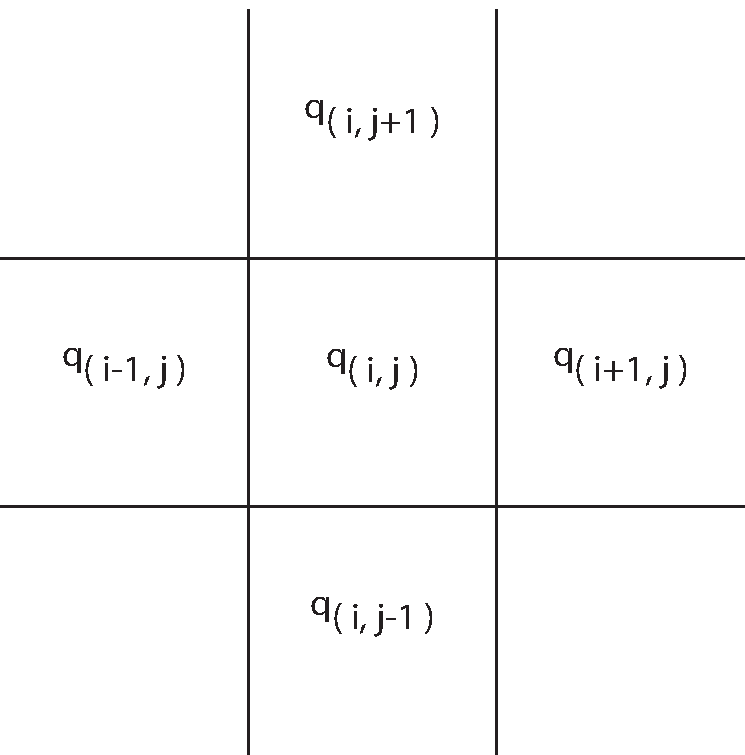
\includegraphics[width=40mm]{img/mac.pdf}
\caption{A grid with quantity $q$ stored at the center of the cells.}
\label{regulargrid}
\end{figure}
\noindent
Before we talk about the difference of a regular grid and a MAC grid, let us revisit derivative approximations. Figure \ref{regulargrid} shows a simple 2D-dimensional grid with the quanity $q_{i,j}$ stored at the center of each cell. To estimate the derivative of q in the x-direction, we can either use first order forward difference 

\begin{equation}
(\frac{\partial q}{\partial x})_{i,j} \approx \frac{q_{i+i,j} - q_{i,j}}{\Delta x}
\end{equation}

accurate to $O(\Delta x)$ or use first order central difference

\begin{equation}
(\frac{\partial q}{\partial x})_{i,j} \approx \frac{q_{i+i,j} - q_{i-1,j}}{2\Delta x}
\label{centraldifference}
\end{equation}

that has accuracy proportional to $O(\Delta x^{2})$. Even though central differencing is more accurate, we can make it even more accurate without having to use complicated approximations. To solve the Navier-Stokes equations later on we are going to need to approximate partial derivatives of both the velocity field $\vec{u}$ and the pressure field $p$. As we will see in later sections of this report, the partial derivative of the pressure field $\frac{\partial p}{\partial x}$ is going to be evaluated to update the velocity field $\vec{u}$. In a similar way, we will have to evaluate $\nabla \cdot \vec{u}$ in the linear equations to solve for pressure. This motivates the use of a staggered grid, i.e a grid where different variables are stored at different locations in the grid.

\begin{figure}[ht!]
\centering
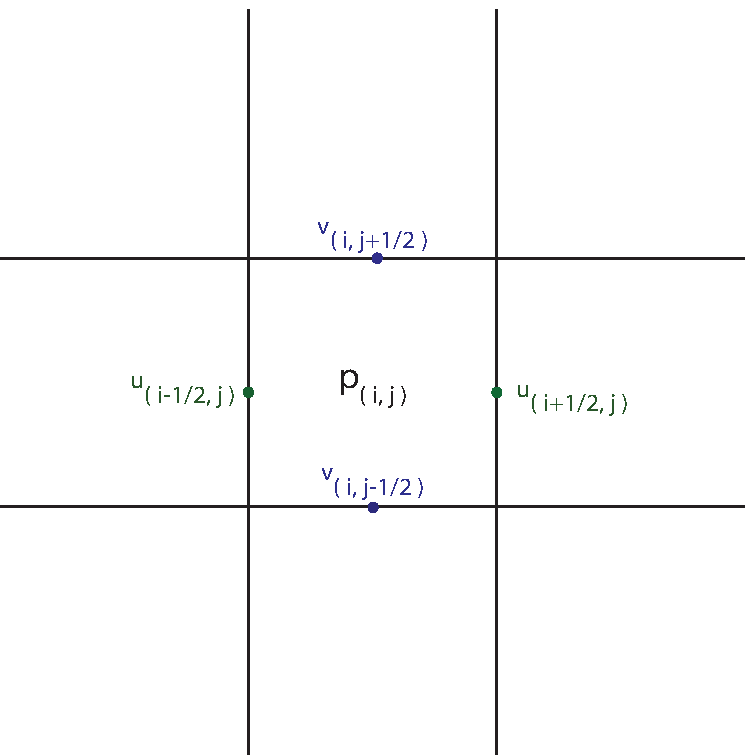
\includegraphics[width=60mm]{img/mac2.pdf}
\caption{A MAC grid with pressure $p$ stored at the center of the cell and velocties $u$ and $v$ stored at the edges.}
\label{macgrid}
\end{figure}
\noindent
In Figure \ref{macgrid} we see a two-dimensional MAC grid. A MAC grid stores the pressure $p$ at the center of the cell and splits the vector field $\vec{u} = (u,v)$ into a component for each axis and store it on the edges of the cell, i.e. in this 2D example it splits $(u,v)$ and stores $u$ on the horizontal edges and $v$ on the vertical ones. At first, this might be confusing but when we evaluate the derivatives it should make more sense. To evaluate the divergence of $\vec{u}$ at the center of a cell $(i,j)$, we use central difference on the values stored at the edges.

\begin{equation}
\nabla \cdot \vec{u} = \frac{u_{i+1/2,j} - u_{i-1/2,j}}{\Delta x} + 
                       \frac{v_{i,j+1/2} - u_{i,j-1/2}}{\Delta x}
\end{equation}
\noindent
Compared to Equation \ref{centraldifference}, we only divide by $\Delta x$ instead of $2\Delta x$. In terms of implementation, the staggered grid does not have a larger memory footprint than a regular grid structure. In other ways, we get more accurate derivatives without slowing down the performance. To evaluate the derivative of the pressure $p$ at a edge we perform central difference on neighboring pressure values stored at the center.

\begin{equation}
\frac{\partial \rho_{i-1/2,j}}{\partial x} = \frac{\rho_{i,j} - \rho_{i-1,j}}{\Delta x}
\end{equation}

\begin{equation}
\frac{\partial \rho_{i,j-1/2}}{\partial y} = \frac{\rho_{i,j} - \rho_{i,j-1}}{\Delta x}
\end{equation}

\subsection{Level Set}

Liquid fluids, unlike gas fluids, have a surface. Tracking a surface is a non-trivial problem to solve due to the complex shape and the evolving change of topology. It is important to get the surface tracking accurate as we later on we need to know if a grid cell is inside, outside or on the surface when solving for pressure. To track the surface, we will use a level set \cite{osher}. A level set is a grid approach to track a surface. At each cell in the grid, a scalar $\phi_{i,j}$ is stored. This absolute value of the scalar tells us the closest distance to the surface. To know if we are inside, outside or on the actual surface we use the following notation:

\begin{equation}
\phi = 
\left\{
\begin{array}{ll}
\phi < 0 & \mbox{inside}  \\
\phi > 0 & \mbox{outside} \\
\phi = 0 & \mbox{surface} \\
\end{array}
\right.
\end{equation}
\noindent
Figure \ref{levetsetexample} shows an example of a surface and a blue interior and a white exterior area. All the cells that have their centers outside of the blue area have positive values and the ones on the inside have negative values. Notice that if the surface is aligned on the center of a cell, $\phi$ is zero.  The further away a cell is from the surface, the larger $| \phi| $ is. 

\begin{figure}[ht!]
\centering
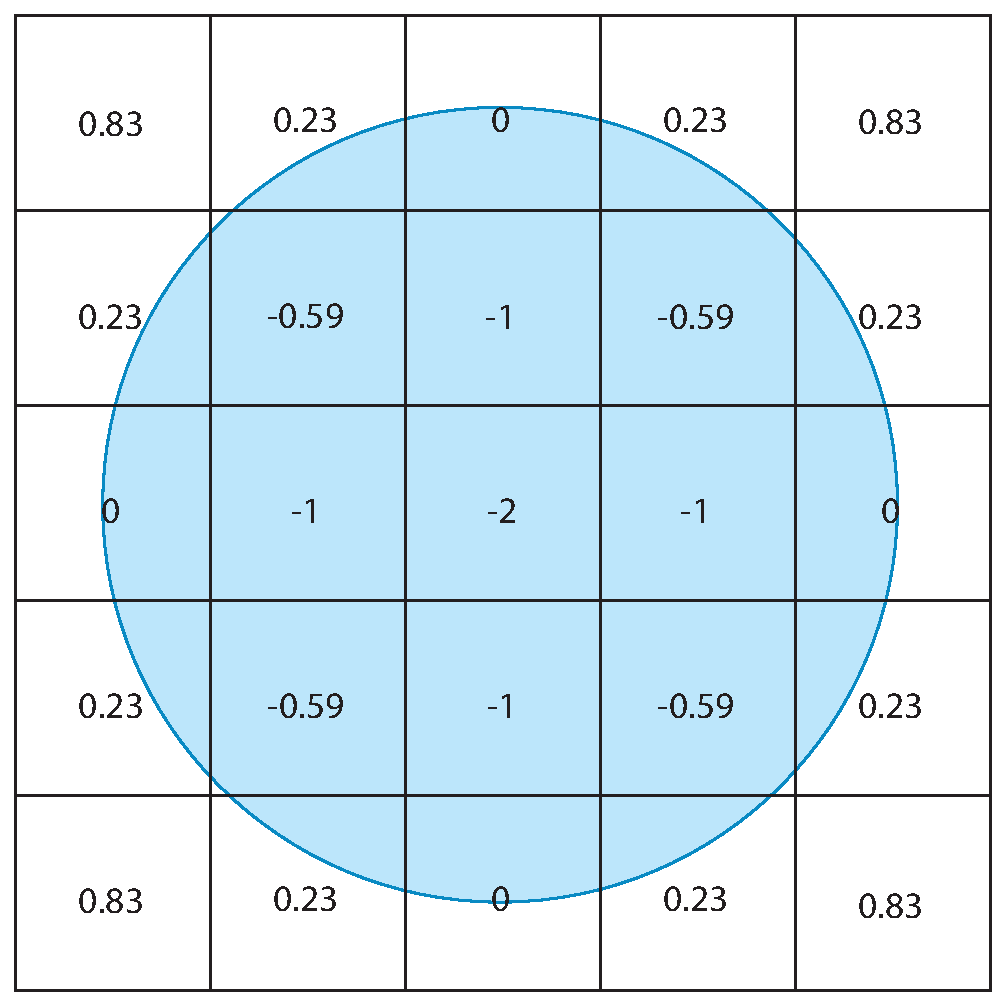
\includegraphics[width=90mm]{img/levelset.pdf}
\caption{A numerical example of a level set representing a sphere (blue).}
\label{levetsetexample}
\end{figure}

Another important feature of a level set is the gradient.

\begin{equation}
\nabla \phi = \hat{n}
\end{equation}

where $\hat{n}$ is the unit vector describing the direction to the closest point of the surface. This means, given spatial coordinates $\vec{x}$, one can easily find the closest point $\vec{x}_s$ on the surface. If we evaluate the level set at $\vec{x}$, i.e. $\phi(\vec{x})$, we get the distance to the surface. If we walk this distance in the negative direction of the gradient, we end up at the surface.

\begin{equation}
\vec{x}_s = \vec{x} - \phi(\vec{x})\nabla \phi(\vec{x})
\end{equation}
\noindent
For any level set operator, it is important that the length of the gradient is always of unit length. This is called the Eikonal equation.

\begin{equation}
|\nabla \phi| = 1
\label{eikonaleqfirst}
\end{equation}

%\subsection{CFL condition}

An important parameter for the simulation is going to be $\Delta t$, i.e how much in time do we step forward after each simulation step. The goal of this report is not to produce real-time simulation but instead focusing on find an as accurate solution as possible. To guarantee that we are not taking too large timestep, we are going to respect the CFL condition. The CFL condition, named after the mathematicians Courant, Friedrichs and Lewy is a condition for convergence which basically says that if you let your timestep $\Delta t$ and sampling size $\Delta x$ in the limit go to zero, then your solution should converge to the exact solution.

In this report we are going to following the same approach mentioned in [REFERENCE] to decide $\Delta t$. The formula to decide the timestep has the following character:

\begin{equation}
\Delta t = \alpha \frac{\Delta x}{max|\vec{u}|}
\label{cfl}
\end{equation}

where $\alpha$ is the CFL number. Note that the CFL number is not the same as the CFL condition. The interpreation of this expression is basically saying that the timestep is restricted so that no information in the grid can be propogated faster than at maximum one grid cell per substep. For example, let us imagine we are advecting temperature $q$ in the vector field and that in one cell, this the temperature is hot. Equation \ref{cfl} says that the hot spot only move at maximum of one grid cell per $\Delta t$ subtep and is guaranteed to not skip cells where the velocity field drasticly change its direction.

\subsection{Outline of the Algorithm}

This section will briefly outline the important steps of the FLIP algorithm that are covered later on in the report. The key to the hybrid FLIP method is that we store both particles and a grid. Each particle stores a position in space, $\vec{x}_p$ and a velocity $\vec{u}_p$. The particles and the grid are going to comminucate and transfer properties to each other. The particles are integrated over time to update the positions. The particle velocities are later transferred to the grid and it is up to the grid to make the velocity field divergence-free and therefore conserving the volume of the water. The input to the algorithm is the initial geometry shape of the fluid and the collidable solid boundaries, i.e. walls or rigid objects that the water should collide against. We will refer to the solid boundaries as just solids in this report. We will use a level set to track the surface of the solids, $\phi_s$. It is trivial to create the solid level set if the we only deal with solids at the grid boundaries. How to create more complex boundaries is not covered in this thesis. More information about creating level sets from arbitrary geometry can be found in \cite{meshtosdf}.

\begin{enumerate}
\item Create particles from initial shape - \emph{Ch 3.1}
\item Transfer particle velocities to grid - \emph{Ch 3.2}
\item Apply external forces to grid
\item Mark cells fluid - \emph{Ch 4.1}
\item Create level set - \emph{Ch 4.1}
\item Reinitialize level set - \emph{Ch 4.2}
\item Extrapolate velocities - \emph{Ch 4.3}
\item Solve pressure equations- \emph{Ch 5}
\item Transfer grid velocities to particles - \emph{Ch 3.3}
\item Advect particles - \emph{Ch 3.4}
\item Repeat step 2-10 until simulation done
\end{enumerate}

The only item not covered later on in this report is \emph{Apply external forces to grid}. This step is straightforward and can be done with a simple Euler step:

\begin{equation}
\vec{u}^{ext} = \vec{u} + \Delta t \cdot \vec{g}
\end{equation}


\newpage
\section{Particles}
\subsection{Creating particles}

Before we run the simulation we need to create the particles representing the volume of the water. To do this we need a function that tells us if a point in space $\vec{x}$ is inside our outside of the initial shape of the water. The distribution of particles depends on the size of the grid used. For a two dimensional cell that is completley inside of the water we create $c_p$ particles. The initial FLIP report suggests the use of $c_p = 4$ with particles jittered from the a subgrid of the cell. Less particles tend to create gaps in the simulation and more particles create unnecessary noise. 

\begin{algorithm}
\caption{Creating particles from an initial water shape}
\begin{algorithmic}
\FOR{$i=0$ to $N_x$}
\FOR{$j=0$ to $N_y$}
\FOR{$k=0$ to $c_p$}
\STATE p = (i,j)$\cdot \Delta x +\frac{random(-1,1) \cdot \Delta x}{2}$
\IF{p is inside water and $\phi_s(p) > 0$}
\STATE create particle at p
\ENDIF
\ENDFOR
\ENDFOR
\ENDFOR
\end{algorithmic}
\label{createalgorithm}
\end{algorithm}

In Algorithm \ref{createalgorithm}, p is a two dimensional vector. {\it random(a,b)} is a function that returns a random value evenly distributed between $a$ and $b$. The $\phi_s > 0$ is a solid level set check to see if the position is outside of the solid.

\begin{figure}[ht!]
\centering
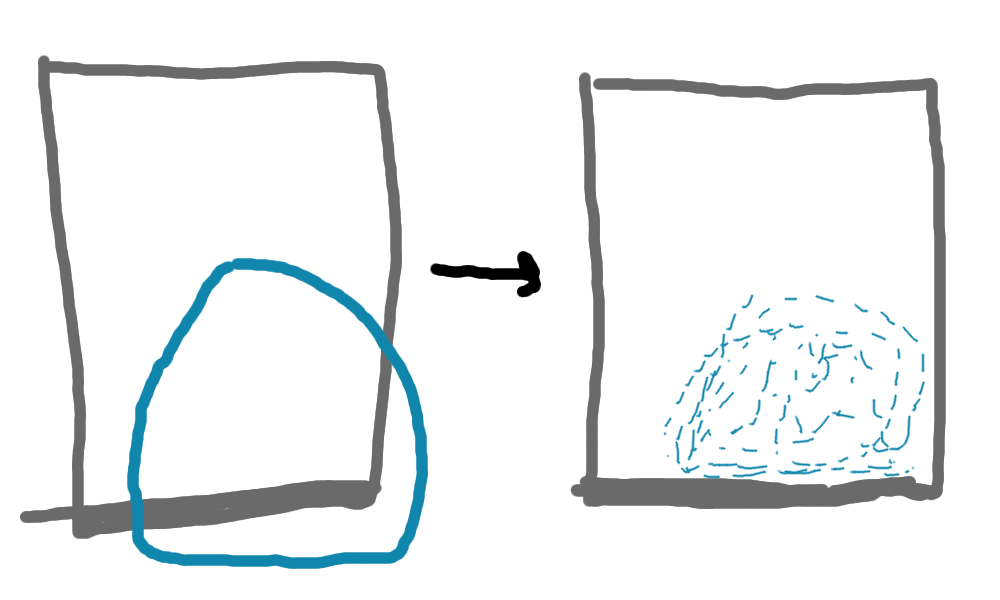
\includegraphics[width=80mm]{ch3/create.png}
\caption{A simple caption}
\label{createexample}
\end{figure}

Figure \ref{createexample} shows a basic example of an initial solid level set $\phi_s$ colored grey and an closed water volume in blue.

\subsection{Transfer particle velocities to grid}

The first thing we need to do after advecting the particles is to transfer the particle velocities to our grid based velocity field. We are going to use the barycentric coordinates of a particle inside a cell to decide how much of the particle velocity is going to affect the neighboring velocities in the MAC grid. Since the velocities $u$ and $v$ are stored on different edges in the MAC grid, we need to be careful when we weight and transfer the particle velocities. The easy case would be when the particle position $\vec{x}_p$ is aligned exactly at the middle of the edge between two cells. Let us compare the difference between $u$ and $v$. 

\begin{figure}[ht!]
\centering
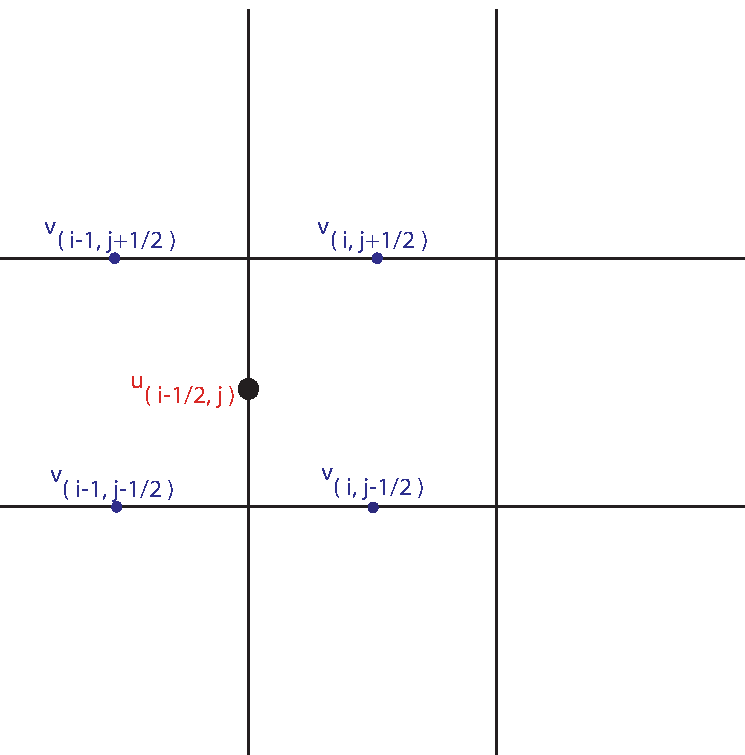
\includegraphics[width=80mm]{img/transfer1.pdf}
\caption{The particle position is aligned exactly at grid position $(i-1/2,j)$.}
\label{onedge}
\end{figure}
\noindent
The particle position $\vec{x}_p$ in Figure \ref{onedge} is exactly at grid position $(i-1/2,j)$. It is reasonable that the horizontal component of the particle velocity $u_p$ only affects the edge at $u_{i-1/2,j}$. The vertical component $v_p$ is not exactly aligned with any vertical edge. This is where the barycentric coordinates come handy. The position $\vec{x}_p$ is exactly in the middle of the rectangle that the vertical edges $v_{i-1,j-1/2}, v_{i,j-1/2}, v_{i-1,j+1/2}, v_{i,j+1/2} $ spans. In this case, it makes sense that the vertical component of the particle velocity $v_p$ should affect the velocity field at all four vertical edges equally much since it it's in the middle of the rectangle.
\begin{figure}[ht!]
\centering
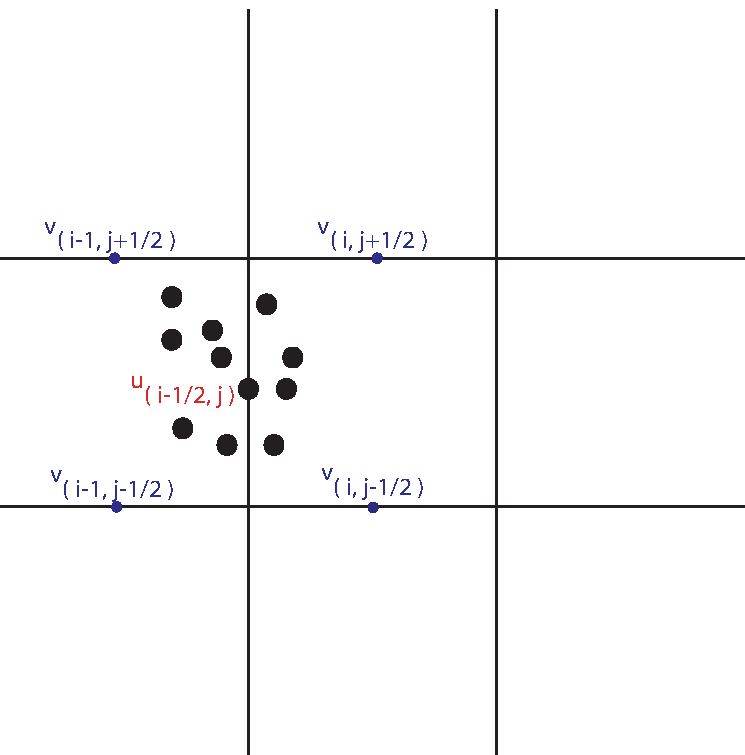
\includegraphics[width=80mm]{img/transfer2.pdf}
\caption{Multiple particles nearby a single horzintal edge at $(i-1/2,j)$.}
\label{fouredge}
\end{figure}
\newline
\newline
\noindent
What if there are multiple particles nearby? How do they all affect the velocities in the grid together? Figure \ref{fouredge} shows a case where multiple particles are close to a single velocity in the MAC grid. We need a way to weight the velocities so that particle velocities closer to an edge have more effect than the ones further away. The final velocity of an edge in the MAC grid is decided by

\begin{eqnarray}
u_{i-1/2,j} = \frac{\sum\limits_{i\in A}\omega_i(x_i) u_{i}}{\sum\limits_{i \in A}\omega_i(x_i)} \\
v_{i,j-1/2} = \frac{ \sum\limits_{i \in B}\lambda_i(x_i) v_{i}}{\sum\limits_{i \in B}\lambda_i(x_i)}
\label{weightsums}
\end{eqnarray}

where $A$ is the set of particles around a horizontal edge and $\omega(x_i)$ is the horizontal weighting function. $B$ is then the set of particles around a vertical edge and $\lambda(x_i)$ is the vertical weighting function.
\begin{figure}[ht!]
\centering
\begin{subfigure}[b]{0.5\textwidth}
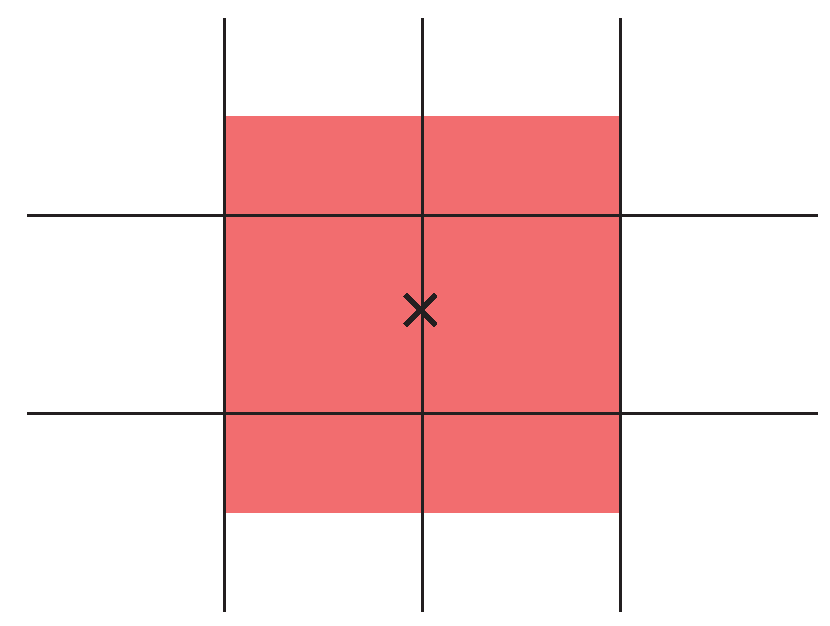
\includegraphics[height=41mm]{img/areau.pdf}
\end{subfigure}
\begin{subfigure}[b]{0.3\textwidth}
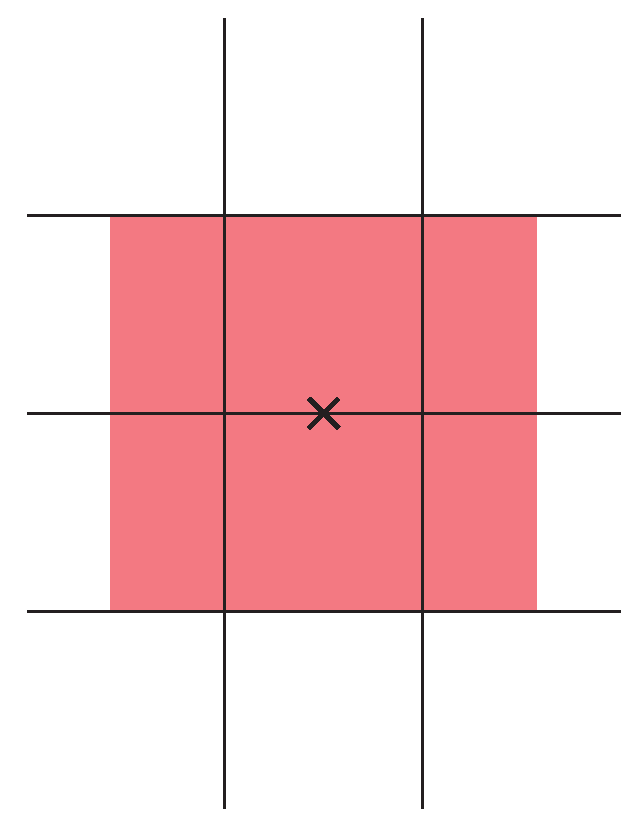
\includegraphics[height=51mm]{img/areav.pdf}
\end{subfigure}
\caption{To the left, the x-marked velocity $u$ at the edge is only updated from particles within the red area. To the right, the x-marked velocity $v$ is only updated from the blue area.}
\label{areaa}
\end{figure}
\newline
\newline
\noindent
Figure \ref{areaa} shows the difference between the sets $A$ and $B$. Updating one edge at a time would require a sophisticated way of only accessing particles close to a specific edge. If not, the time complexity for gathering particles in $A$ and $B$ would be $O(n)$ for each edge where $n$ is the total number of particles in the simulation. Instead, we will use a technique called splatting. In splatting approaches, you iterate over all the particles instead of all the grid cells. For each particle, we find out which edges it could affect. This is fast since each particle has a position and $A$ and $B$ have a fixed maximum size. The splatting method is divided into two parts. Part one can be seen in Algorithm \ref{particlestogridalgorithm1}. Notice that there is a temporary $sum$ MAC grid for storing the denominator part of Equation \ref{weightsums}.
\begin{algorithm}
\caption{Step one in splatting particle velocities to grid velocities}
\begin{algorithmic}
\STATE grid = empty mac grid
\STATE sum = empty mac grid
\FOR{all particles $p$}
\STATE tx,ty = barycentricA(p.x)
\FOR{neighboring horizontal edges $e$}
\STATE weight = omega(tx,ty, p.x)
\STATE grid.u[e.idx] += weight * p.u
\STATE sum.u[e.idx] += weight
\ENDFOR
\STATE tx,ty = barycentricB(p.x)
\FOR{neighboring vertical edges $e$}
\STATE weight = lambda(tx,ty, p.x)
\STATE grid.v[e.idx] += weight * p.v
\STATE sum.v[e.idx] += weight
\ENDFOR
\ENDFOR
\end{algorithmic}
\label{particlestogridalgorithm1}
\end{algorithm}
\newline
\newline
\noindent
The barycentric functions in Algorithm \ref{particlestogridalgorithm1} returns two normalized coordinates from $0$ to $1$ where bottom left of the region gives back $(0,0)$, bottom right $(1,0)$, top left $(0,1)$ and top right $(1,1)$. Anything in between is linearly interpolated.
\begin{algorithm}
\caption{Step two in splatting particle velocities to grid velocities}
\begin{algorithmic}
\FOR{$i=0$ to $N_x$}
\FOR{$j=0$ to $N_y$}
\STATE idx = .... get index for (i-1/2,j)
\STATE grid.u[idx] /= sum.u[idx]
\STATE idx = ... get index for (i,j-1/2)
\STATE grid.v[idx] /= sum.v[idx]
\ENDFOR
\ENDFOR
\end{algorithmic}
\label{particlestogridalgorithm2}
\end{algorithm}
\newline
\newline
\noindent
The second step of the splatting process is to normalize all the velocities. In Algorithm \ref{particlestogridalgorithm1} we only applied the numerator of Equation \ref{weightsums}. Once all velocities are splatted we also have the sum of all weights. If we divide the current edge velocity with the sum stored at each edge,  Equation \ref{weightsums} is true and the transfer from particles to grid is done.

\subsection{Transfer grid velocities to particles}

As we could see in the previous section, going from particle velocities to grid can be a bit tricky when working with a MAC grid. Luckily, going from grid velocities to particle velocities is a lot easier. For every particle, we will use bilinear interpolation to get the horizontal and vertical velocities.

\begin{figure}[ht!]
\centering
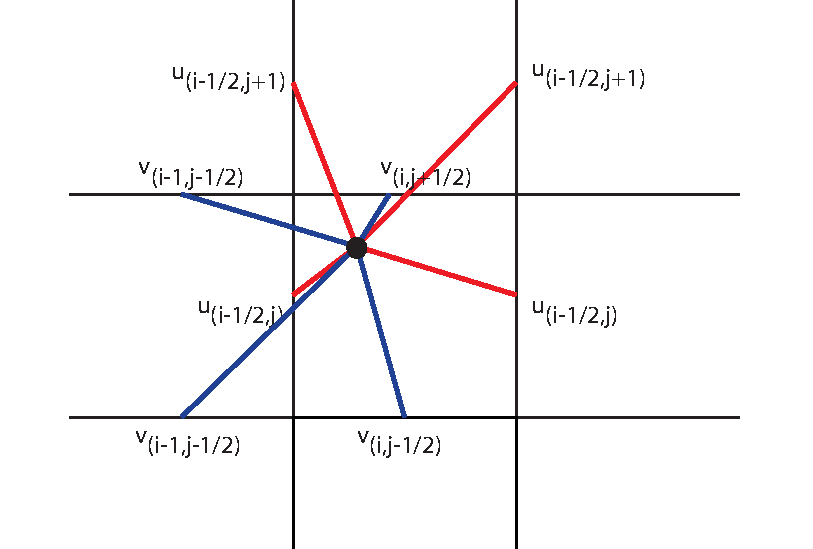
\includegraphics[width=80mm]{img/splat.pdf}
\caption{The particle velocity $\vec{u}_p$ is bilineary interpolated between neighboring velocities in the MAC grid.}
\label{onedge}
\end{figure}
\noindent
The FLIP part of our hybrid particle-grid approach is how we update the particle velocities. If we only update the particles with the velocities that the pressure solving step gives us, it is called \emph{Particle in Cell}, PIC, which is an older approach. Zhou and Bridson \cite{chu} are in their FLIP paper, before solving the pressure equations, saving the old divergence-free velocity field and then updating the particles with the change of velocity instead of only the new velocity.

\begin{equation}
\Delta \vec{u} = \vec{u}^{n+1} - \vec{u}^n
\end{equation}
\noindent
FLIP alone can cause a lot of noise because of the large particle count. The FLIP paper recommends linear interpolation between FLIP and PIC for best result. The formula for updated particle velocities can be expressed as:

\begin{equation}
\vec{u}_p = \alpha \cdot bilerp(\vec{u}^{n+1}, \vec{x}_p) + (1-\alpha) \cdot bilerp(\Delta \vec{u},\vec{x}_p)
\label{flipeq}
\end{equation}

where $\alpha$ is a number between $0$ and $1$. If one, it is only PIC and zero is pure FLIP. Values closer to one gives a more stable look but to the cost of more numerical dissipation which cancels out a lot of the interesting high frequency motion.

\subsection{Advecting particles}

The most straight forward approach to update particle positions ${\vec{x}_p}^{n+1}$ is to use simple forward Euler time integration on the velocities given from Equation \ref{flipeq}. 

\begin{equation}
{\vec{x}_p}^{n+1} = {\vec{x}_p}^n + \Delta t \vec{u}_p 
\label{eulerstepeq}
\end{equation}
\noindent
We can improve accuracy by using a different time integration scheme. First we need Equation \ref{flipeq} to be a function that uses an arbitrary position $\vec{x}$ as input and not the position from each particle $\vec{x}_p$. We call this function $vel(\vec{x})$.

\begin{equation}
vel(\vec{x}) = \alpha \cdot bilerp(\vec{u}^{n+1}, \vec{x}) + (1-\alpha) \cdot bilerp(\Delta \vec{u},\vec{x})
\label{veleq}
\end{equation}
\noindent
We are going to use a second order Runge-Kutta method where we evaluate a mid point and use the mid point to evaluate the velocity of the particle rather than the position of the particle.

\begin{equation}
{\vec{x}_p}^{n + 1/2} = {\vec{x}_p}^n + \frac{\Delta t}{2} vel(\vec{x}_p)
\label{halfstepeq}
\end{equation}
\noindent
Note that we only use half of the timestep $\Delta t$ in Equation \ref{halfstepeq} to evaluate the in-between position ${\vec{x}_p}^{n+1}$. The final position of a particle in each step can then be set to

\begin{equation}
{\vec{x}_p}^{n + 1} = {\vec{x}_p}^n + \Delta t \cdot vel({\vec{x}_p}^{n+1/2})
\end{equation}
\noindent
After advecting the particles we still need to run a correction step in case some of the particles get stuck in the solid $\phi_s$. The boundary condition of the pressure equations (covered later in this report) are supposed to prevent this from happening but due to numerical errors in our single precision simulation there are still going to be cases where particles intersect the solid. If this is the case, we move the particle out in the normal direction of the solid.

\begin{equation}
{\vec{x}_p}^{correction} = \vec{x}_p + \beta |\phi_s|\nabla\phi_s
\end{equation}

with $\beta > 1$. If $\beta$ would be exactly 1 then we would only move the particle to surface of the solid. In the implementation, $\beta = 1.5$ was used.


\newpage
\section{Surface tracking}
\subsection{Creating the Level Set}

Before we create the level set $\phi$ that represent the surface of our water simulation, we need to mark the cells we consider being fluid. The easiest approach is to go from particle position $\vec{x}_p$ to grid coordinates $(i,j)$ and tag the cell with those coordinates as fluid.

\begin{algorithm}
\caption{Marking cells as fluid}
\begin{algorithmic}
\STATE marker = empty grid (all values 0)
\FOR{all particles $p$}
\STATE i,j = int(p.x / $\Delta x$)
\STATE marker(i,j) = 1
\ENDFOR
\end{algorithmic}
\label{markalgorithm}
\end{algorithm}
\noindent
In Algorithm \ref{markalgorithm}, a cell will most likely contain several particles at once which means that we will write the value $1$ to that cell multiple times. Although unnecessary, this is a very fast operation compared to all the other steps in the level set creation and the overhead is not noticeable. Figure \ref{markerexample} shows an example of the marker grid after we run Algorithm \ref{markalgorithm} on an input of particles. Notice that cells with only one particle is still counted as a fluid cell.

\begin{figure}[ht!]
\centering
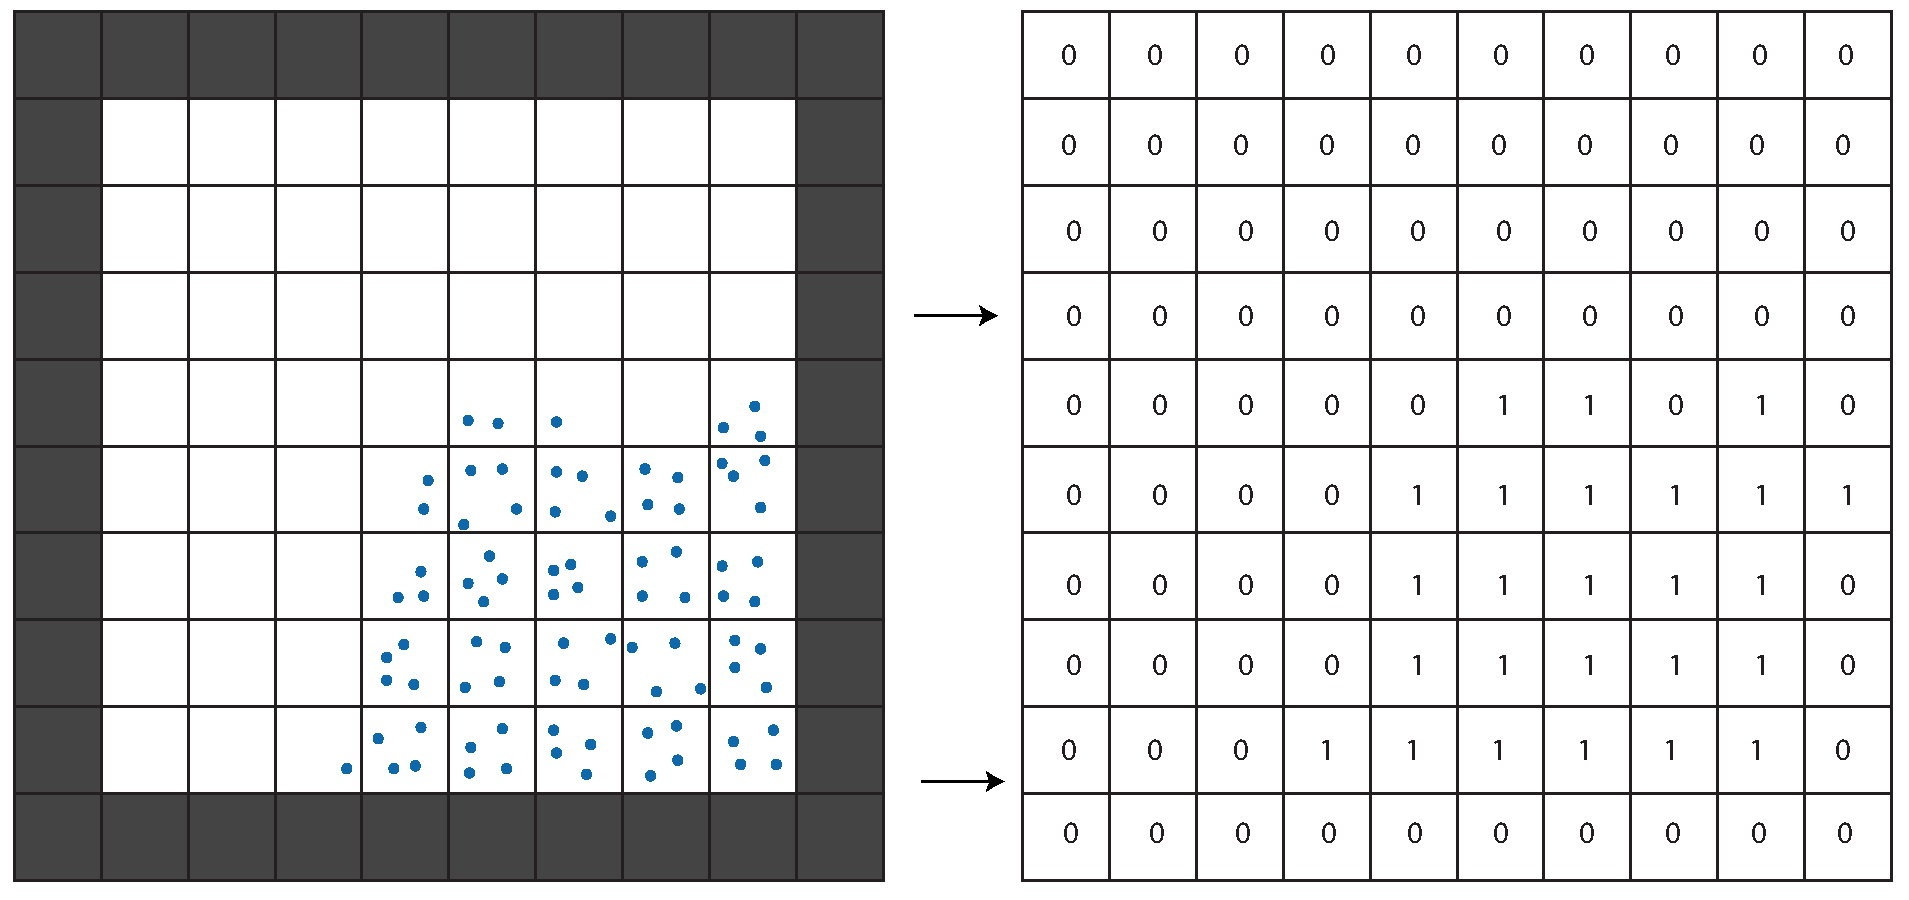
\includegraphics[width=130mm]{img/mark.pdf}
\caption{Cells with particles inside them as are marked as fluid cells.}
\label{markerexample}
\end{figure}
\noindent
Then next step in the algorithm is to initialize the level set. This step will not create a valid level set that satisfies Equation \ref{eikonaleqfirst}. To start with, we set $\phi_{i,j}$ to $-\frac{\Delta x}{2}$ as if the surface could be at the edge of the cell. To cells not marked as fluid we set the value to $D \cdot \Delta x$ where it is important that $D >> \Delta x$. Typically the initializing step is run with $D = 1000$.

\begin{algorithm}
\caption{Initalizing the Level Set}
\begin{algorithmic}
\STATE marker = ... (marker grid from Algorithm \ref{markalgorithm})
\STATE inside = -0.5 * $\Delta x$
\STATE outside = D * $\Delta x$
\FOR{$i=0$ to $N_x$}
\FOR{$j=0$ to $N_y$}
\IF{marker(i,j) is 1}
\STATE phi(i,j) = inside
\ELSE
\STATE phi(i,j) = outside
\ENDIF
\ENDFOR
\ENDFOR
\end{algorithmic}
\label{particlestogridalgorithm2}
\end{algorithm}
\noindent
After the initializing step, the level set is far from continuous. To make it continuous and satisfy $|\nabla \phi| = 1$, we are going to iteratively solve the Eikonal equation. This step is sometimes called the reinitializing step in level set literature.

\subsection{Reinitializing the Level Set}

The goal of the reinitializing step is to make sure that the gradient of the level set is always a unit vector, i.e the length is 1. To do this we will use a method called fast sweeping, which sweeps and propagates the solution of an iterative approach in different directions. Before we go into detail about the fast sweeping algorithm itself, let us write down and evaluate tha gradient of $\phi$ and the Eikonal equation in two dimensions

\begin{equation}
\nabla \phi = (\frac{\partial \phi}{\partial x}, \frac{\partial \phi}{\partial y})
\end{equation}

\begin{equation}
\begin{split}
|\nabla \phi| &= \sqrt{{(\frac{\partial \phi}{\partial x})}^2 + {(\frac{\partial \phi}{\partial y})}^2}  = 1
\end{split}
\label{evaleiokanl}
\end{equation}
\noindent
We can now turn Equation \ref{evaleiokanl} into an discrete version and therefore making it possible to solve it iteratively. Let us approximate the partial derivatives with backward differences

\begin{equation}
\begin{split}
\frac{\partial \phi}{\partial x} &\approx \frac{\phi_{i,j} - \phi_{i-1,j}}{\Delta x} \\
\frac{\partial \phi}{\partial y} &\approx \frac{\phi_{i,j} - \phi_{i,j-1}}{\Delta x}
\end{split}
\label{phiapproxeq}
\end{equation}
\noindent
If we square both the left and right hand side of Equation \ref{evaleiokanl} and use the approximations of the partial derivatives, we get

\begin{equation}
\begin{split}
{(\frac{\phi_{i,j} - \phi_{i-1,j}}{\Delta x})}^2 + {(\frac{\phi_{i,j} - \phi_{i,j-1}}{\Delta x})}^2 &= 1 \\ 
({\phi_{i,j}}^2 - 2\phi_{i,j}\phi_{i-1,j} + {\phi_{i-1,j}}^2) + 
({\phi_{i,j}}^2 - 2\phi_{i,j}\phi_{i,j-1} + {\phi_{i,j-1}}^2)
&= {\Delta x}^2 \\
2{\phi_{i,j}}^2 - 2\phi_{i,j}(\phi_{i-1,j} + \phi_{i,j-1}) + {\phi_{i-1,j}}^2 + {\phi_{i,j-1}}^2 - {\Delta x}^2 &= 0 \\
{\phi_{i,j}}^2 - \phi_{i,j}(\phi_{i-1,j} + \phi_{i,j-1}) + \frac{{\phi_{i-1,j}}^2 + {\phi_{i,j-1}}^2 - {\Delta x}^2}{2} &= 0
\end{split}
\label{phisimplified}
\end{equation}
\noindent
To simplify things, let us store the non $\phi_{i,j}$ parts in temporary variables
\begin{equation}
\begin{split}
b &= \phi_{i-1,j} + \phi_{i,j-1} \\
c &= \frac{{\phi_{i-1,j}}^2 + {\phi_{i,j-1}}^2 - {\Delta x}^2}{2}
\end{split}
\label{variablesreinit}
\end{equation}
\noindent
Equation \ref{phisimplified} can then be put on the form

\begin{equation} 
{\phi_{i,j}}^2 - \phi_{i,j} b + c = 0
\end{equation}

which is a standard quadratic equation. Rearranging the terms we get

\begin{equation} 
\begin{split}
{\phi_{i,j}}^2 - \phi_{i,j} b + c &= 0 \\
{(\phi_{i,j} - \frac{b}{2})}^2  = b^2 - c \\
\phi_{i,j} =  \frac{b}{2} \pm \sqrt{b^2 - c}
\end{split}
\label{solvephi}
\end{equation}
\noindent
If $b^2 - c < 0$, we do not update $\phi_{i,j}^{n+1}$. If $b^2 - c > 0$, Equation \ref{solvephi} has two real solutions ${\phi_{i,j}}^a$ and ${\phi_{i,j}}^b$. We pick the smaller value of the two as our solution. 

\begin{equation}
{\phi_{i,j}}^{new} = min({\phi_{i,j}}^a, {\phi_{i,j}}^b)
\end{equation}
\noindent
Another condition we use is that new solution to ${\phi_{i,j}}^{new}$ has to be smaller than the previous value ${\phi_{i,j}}^{n}$. This is why it was important to pick $D >> \Delta x$. It means that we are only propagating the level set from the surface and inwards/outwards and not from the center of the fluid towards the surface.

\begin{equation}
{\phi_{i,j}}^{n+1} = 
\left\{
\begin{array}{ll}
{\phi_{i,j}}^{new} & \mbox{if ${\phi_{i,j}}^{new} < {\phi_{i,j}}^{n}$} \\
{\phi_{i,j}}^{n} & \mbox{if ${\phi_{i,j}}^{new} > {\phi_{i,j}}^{n}$}
\end{array}
\right.
\end{equation}
\noindent
Now that we have an iterative way of solving the Eikonal equation, let us talk more about the fast sweeping method. Fast sweeping for solving the Eikonal equation was introduced by Zhao\cite{zhao}. The fundamentals of the method are that you sweep your domain in every possible direction which tells you in which order to update the cells. In a two dimensional case, there are only four different directions:

\begin{itemize}
\item left to right, bottom to top
\item left to right, top to bottom
\item right to left, bottom to top
\item right to left, top to bottom
\end{itemize}
\noindent
Depending on the sweeping order, the approximation of the partial derivatives in Equation \ref{phiapproxeq} is different. The goal with fast sweeping is to use updated data from the same sweep and therefore have faster convergence. For example, if we are sweeping from left to right, it makes sense to approximate the horizontal partial derivative with $\phi_{i,j} - \phi_{i-1,j}$ since $\phi_{i-1,j}$ was just updated. However, if we are sweeping from right to left, then it is better to approximate the horizontal partial derivative with $\phi_{i,j} - \phi_{i+1,j}$. We need to take this into account when we are solving Equation \ref{solvephi}.

\begin{equation}
\frac{\partial \phi}{\partial x} \approx
\left\{
\begin{array}{ll}
\frac{\phi_{i,j} - \phi_{i-1,j}}{\Delta x} & \mbox{if horizontal sweeping is left to right} \\
\frac{\phi_{i,j} - \phi_{i+1,j}}{\Delta x} & \mbox{if horizontal sweeping is right to left} \\
\end{array}
\right.
\end{equation}

\begin{equation}
\frac{\partial \phi}{\partial y} \approx
\left\{
\begin{array}{ll}
\frac{\phi_{i,j} - \phi_{i,j-1}}{\Delta x} & \mbox{if vertical sweeping is bottom to top} \\
\frac{\phi_{i,j} - \phi_{i,j+1}}{\Delta x} & \mbox{if vertical sweeping is top to bottom} \\
\end{array}
\right.
\end{equation}

Figure \ref{sweeppic} shows an example of the update order when sweeping from left to right and bottom to right.

\begin{figure}[ht!]
\centering
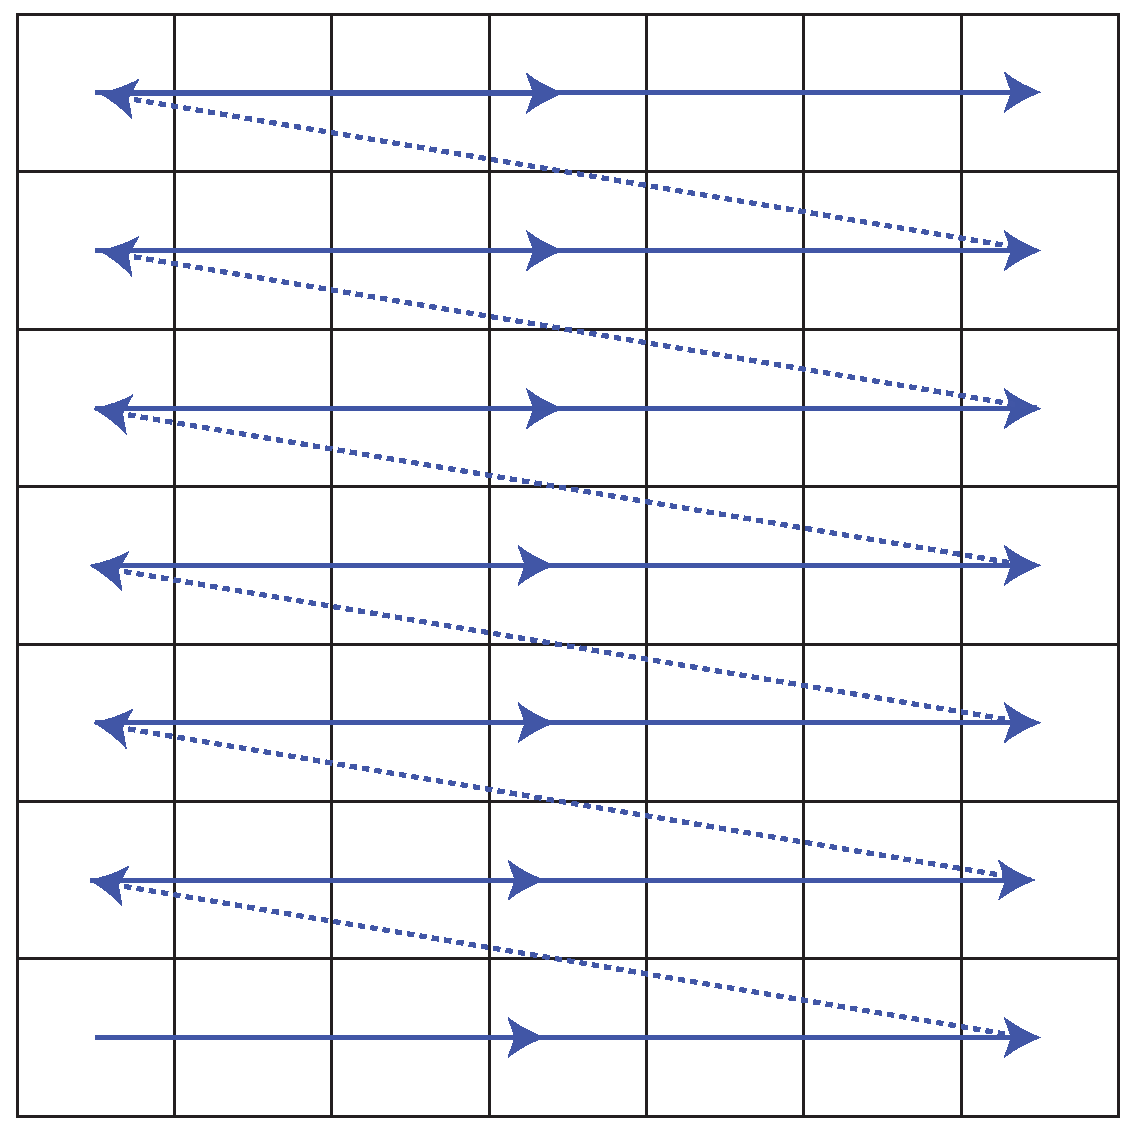
\includegraphics[width=80mm]{img/sweep.pdf}
\caption{Left to right, bottom to top sweeping order. In an iterative solver, the cells are updated in the order of the blue arrows.}
\label{sweeppic}
\end{figure}

\subsection{Extrapolate velocities}

Sometimes it happens that an edge on the grid is close to the surface but no particle was close enough to update the velocity of the edge. We have to be able to guarantee that we have valid velocities on the grid where the level set tells us an edge inside or close to the surface of the fluid. To ensure this, we will extrapolate the velocities from the surface and outwards with the help of the level set. Remember from section 2.3 that the gradient of the level set is the same as the normal of the surface. If we extrapolate the velocities in the direction of the normal, the derivative of the velocities along the normal should be zero. We can use this condition to create an iterative solution to the unknown velocities outside of the surface. The following equations say that the horizontal velocity $u$ should be constant along the normal of the surface.
\begin{equation}
\begin{split}
\nabla \phi \cdot \nabla u &= 0 \\
\frac{\partial \phi}{\partial x}\frac{\partial u}{\partial x} + 
\frac{\partial \phi}{\partial y}\frac{\partial u}{\partial y}&= 0
\end{split}
\label{extrapolate}
\end{equation}
\noindent
To find an expression that we can solve iteratively we need to approximate the partial derivatives similar to what we did in previous section. We can then use the fast sweeping method once more. Notice that Equation \ref{extrapolate} is only for the horizontal velocities $u$ and one has to solve vertical velocities $v$ individually. It is important that the fast sweeping algorithm only updates velocities on edges that did not receive any velocities from the particles because we do not want the velocity field to be constant in the negative direction of the normal.
\begin{figure}[ht!]
\centering
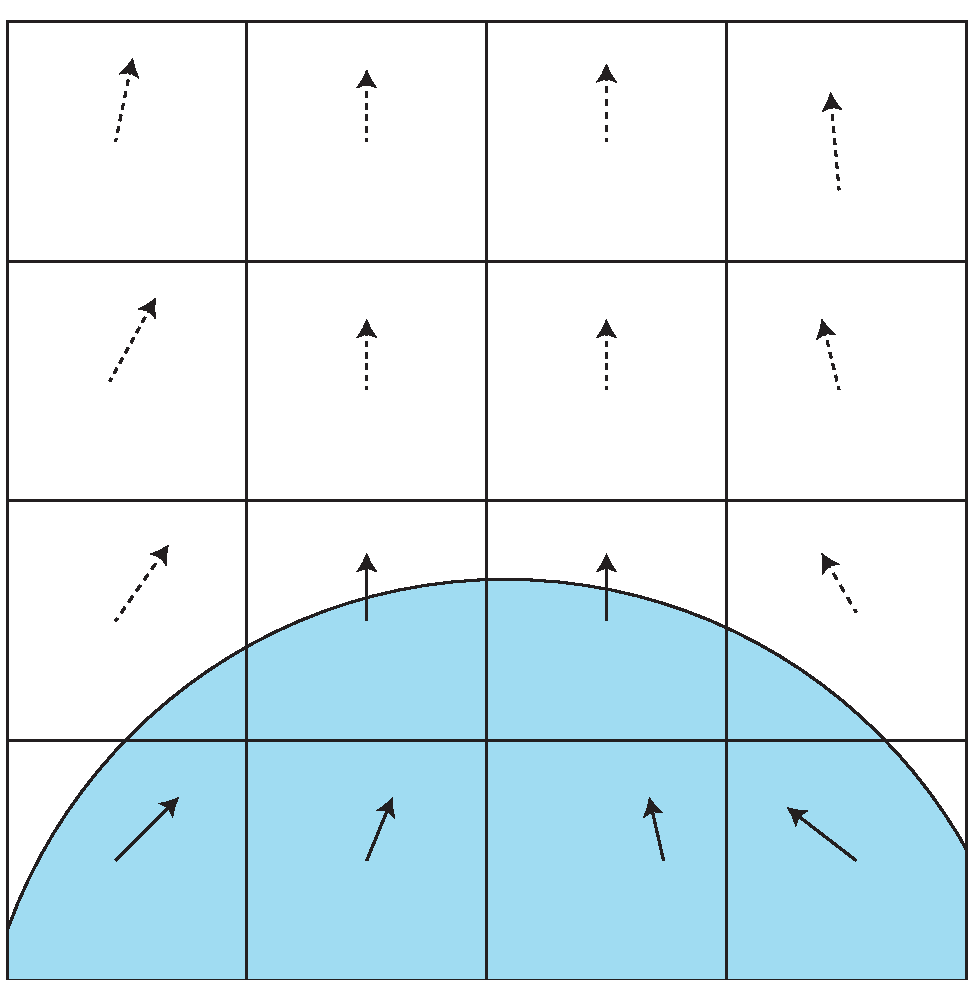
\includegraphics[width=50mm]{img/extrapolate.pdf}
\caption{The velocities of the cells inside the fluid (marked as solid arrows) are extrapolated in the surface normal direction (marked as dashed arrows).}
\label{extrapic}
\end{figure}


\newpage
\section{Solving for pressure}
To guarantee the velocity field is divergence free we need to solve the pressure equations. This step is called the Projection step. We are going to use an approach Alexandre Chorin introduced in 1967 \cite{chorin}. The key is to split the Euler fluid equations into two steps and solve the sequentially. In the first step we solve for the intermediate velocity field $\vec{u}^*$. This vector field is not divergence free but we use it as an input to the second step of the splitting. We will set up the pressure equations later on in such way that removing the pressure gradient $\nabla p$ from the intermediate $\vec{u}^*$ will make $\vec{u}^{n+1}$ divergence-free.

\begin{equation}
\vec{u}^{n+1} = \vec{u}^* - \frac{\Delta t}{\rho} \nabla p
\label{pressuredivfreeeq}
\end{equation}

If we rearrange Equation \ref{pressuredivfreeeq}, we get a substitution for the pressure term in the Euler fluid equations described in Equation \ref{eulereq}.

\begin{equation}
\frac{\vec{u}^{n+1} - \vec{u}^*}{\Delta t}= - \frac{1}{\rho} \nabla p
\label{pressuredivfreeeq}
\end{equation}

If we approximate $\frac{\partial \vec{u}}{\partial t}$ with $\frac{\vec{u}^{n+1} - \vec{u}^{n}}{\Delta t}$, we can rewrite Equation \ref {eulereq} to

\begin{equation}
\begin{split}
\frac{\partial \vec{u}}{\partial t}  &= -\vec{u} \cdot \nabla \vec{u} - \frac{1}{\rho}\nabla p + \vec{f}\\
\frac{\vec{u}^{n+1} - \vec{u}^{n}}{\Delta t}  &= - \vec{u} \cdot \nabla \vec{u} + \frac{\vec{u}^{n+1} - \vec{u}^*}{\Delta t} + \vec{f} \\
\vec{u}^* & = \vec{u}^n - \Delta t(\vec{u} \cdot \nabla \vec{u}) + \Delta t\vec{f}
\end{split}
\end{equation}

In our hybrid FLIP simulation, getting the intermediate velocity field  $\vec{u}^*$ each substep is easy where the Lagrangian particle update gives the use the advection terms and the applying the integrated force $\vec{f}$ over timestep $\Delta t$ is trivial. The tricky part of the pressure solving step is setting up the pressure equations that enforces an incompressible fluid.

\subsection{Setting up the Pressure Equations}

Before setting up the linear systems for solving the pressure, let us look at the discrete implementation of Equation \ref {pressuredivfreeeq}. The use of MAC grid once again comes in handy since it makes the use of central difference approximations easy and more robust. For each dimension, we perform an pressure update to the velocity field $\vec{u}^{n+1}$ the following way:

\begin{equation}
\begin{split}
{u^{n+1}}_{i+1/2,j} &= {u^*}_{i+1/2,j} - \frac{\Delta t }{\rho}\frac{p_{i+1,j} - p_{i,j}}{\Delta x} \\
{u^{n+1}}_{i-1/2,j} &= {u^*}_{i-1/2,j} - \frac{\Delta t }{\rho}\frac{p_{i,j} - p_{i-1,j}}{\Delta x} \\
{v^{n+1}}_{i,j+1/2} &= {v^*}_{i,j+1/2} - \frac{\Delta t }{\rho}\frac{p_{i,j+1} - p_{i,j}}{\Delta x} \\
{v^{n+1}}_{i,j-1/2} &= {v^*}_{i,j-1/2} - \frac{\Delta t }{\rho}\frac{p_{i,j} - p_{i,j-1/2}}{\Delta x}
\end{split}
\label{pressurefaceupdateeq}
\end{equation}

The most important condition is the imcompressible one. We have to guarantee that for every cell in the grid the next velocity field $\vec{u}^{n+1}$is divergence free. If we evaluate the divergence-free condition for a cell on our MAC grid we get the following:

\begin{equation}
\frac{{u^{n+1}}_{i+1/2,j} - {u^{n+1}}_{i-1/2,j}}{\Delta x} + \frac{{v^{n+1}}_{i,j+1/2} - {v^{n+1}}_{i,j-1/2}}{\Delta x} = 0
\end{equation}

If we replace the velocities for next step $(n+1)$ with the right hand sides of Equation \ref{pressurefaceupdateeq}, we get

\begin{equation}
\begin{split}
\frac{1}{\Delta x}[ &{u^*}_{i+1/2,j} - \frac{\Delta t }{\rho}\frac{p_{i+1,j} - p_{i,j}}{\Delta x}
\\
& - {u^*}_{i-1/2,j} + \frac{\Delta t }{\rho}\frac{p_{i,j} - p_{i-1,j}}{\Delta x} \\
& + {v^*}_{i,j+1/2} - \frac{\Delta t }{\rho}\frac{p_{i,j+1} - p_{i,j}}{\Delta x} \\
& -{v^*}_{i,j-1/2} + \frac{\Delta t }{\rho}\frac{p_{i,j} - p_{i,j-1/2}}{\Delta x} ] = 0
\end{split}
\label{pressurebeforeeq}
\end{equation}

If we rearrange the terms in Equation \ref{pressurebeforeeq} we get an expression that is more intuitive to put in a linear system of equations.

\begin{equation}
\begin{split}
4p_{i,j} - p_{i-1,j} - p_{i+1,j} & - p_{i,j-1} - p_{i,j+1} = \\ &-\frac{\rho \Delta x}{\Delta t}({u^*}_{i+1/2,j} - {u^*}_{i-1/2,j} + {v^*}_{i,j+1/2} - {v^*}_{i,j-1/2})
\end{split}
\label{pressureeq}
\end{equation}

\subsection{Boundary conditions}

There are two different kinds of boundary conditions we must take into account before we build our linear system. The first one is on the boundary between air and the fluid, also called as the free surface boundary condition. Air is a lot lighter than water (the density of water is approximately 700 larger than air) and we make the simplification in our model that air can be represented with constant atmospheric pressure (in reality air is also a fluid). Equation \ref{eulereq} tells us that only the derivative of pressure matters when updating our velocity field which means it does not matter which constant we use for air since the derivative is going to be zero. For convenience, we choose pressure to be zero for every air cell. When enforcing a constant at the boundary, it is called a Dirichlet boundary condition. In Equation \ref{pressureeq}, if a neighboring cell is air, we force the pressure of that cell to be zero. For example, when setting up the pressure equations for cell $(i,j)$, let us say that cell $(i-1, j)$ is an air cell. The pressure equation for cell $(i,j)$ is then changed to

\begin{equation}
\begin{split}
4p_{i,j} - 0 - p_{i+1,j} & - p_{i,j-1} - p_{i,j+1} = \\ &-\frac{\rho \Delta x}{\Delta t}({u^*}_{i+1/2,j} - {u^*}_{i-1/2,j} + {v^*}_{i,j+1/2} - {v^*}_{i,j-1/2})
\end{split}
\label{dirichleteq}
\end{equation}
\noindent
The more difficult boundary condition is the one between the fluid and the solid. In terms of our velocity field, it is important that no fluid is flowing into the solid. This means that the normal component of the velocity has to be zero

\begin{equation}
\vec{u} \cdot \hat{n} = 0
\end{equation}
\noindent
In our implementation we are going to enforce the velocity of every edge next to a solid cell to be zero after updating the pressure. The confusing part is to understand how solid boundaries change the pressure equation. To find an expression for pressure in neighboring solid cells, let us start with an example where cell $(i,j)$ is a fluid and cell $(i+1,j)$. We want to guarantee that $u^{n+1}_{i+1/2,j} = 0$ after the pressure update, which means we can rewrite Equation \ref{pressurefaceupdateeq} to

\begin{equation}
0 = {u^*}_{i+1/2,j} - \frac{\Delta t }{\rho}\frac{p_{i+1,j} - p_{i,j}}{\Delta x}
\label{solidveleq}
\end{equation}
\noindent
If we rearrange the terms we get an expression for the pressure inside the solid, $p_{i+1,j}$.
\begin{equation}
p_{i+1,j} = p_{i,j} + \frac{\rho \Delta x}{\Delta t}{u^*}_{i+1/2,j}
\label{solidpressureeq}
\end{equation}
\noindent
In this example, where cell $(i,j)$ has one solid neighboring cell at $(i+1,j)$ and three neighboring fluid cells, we substitute $p_{i+1,j}$ in Equation \ref{pressureeq} with the right hand side of Equation \ref{solidpressureeq} to get

\begin{equation}
\begin{split}
4p_{i,j} - p_{i-1,j} - &(p_{i,j} + \frac{\rho \Delta x}{\Delta t}{u^*}_{i+1/2,j}) - p_{i,j-1} - p_{i,j+1} = \\ &-\frac{\rho \Delta x}{\Delta t}({u^*}_{i+1/2,j} - {u^*}_{i-1/2,j} + {v^*}_{i,j+1/2} - {v^*}_{i,j-1/2})
\end{split}
\label{solidpressureeqfull}
\end{equation}

which can be simplified to
\begin{equation}
3p_{i,j} - p_{i-1,j} - p_{i,j-1} - p_{i,j+1} = -\frac{\rho \Delta x}{\Delta t}(- {u^*}_{i-1/2,j} + {v^*}_{i,j+1/2} - {v^*}_{i,j-1/2})
\end{equation}
\noindent
We now have everything we need to know to build a linear system of the pressure equations $A\vec{p} = \vec{b}$.

\begin{algorithm}
\caption{Building right hand side $b$}
\begin{algorithmic}
\STATE b = empty grid
\STATE scale = $-\frac{\rho\Delta x}{\Delta t}$
\FOR{$i=0$ to $N_x$}
\FOR{$j=0$ to $N_y$}
\IF{cell $(i-1,j)$ is not solid}
\STATE b(i,j) += ${u^*}_{i-1/2,j}$
\ENDIF
\IF{cell $(i+1,j)$ is not solid}
\STATE b(i,j) += ${u^*}_{i+1/2,j}$
\ENDIF
\IF{cell $(i,j-1)$ is not solid}
\STATE b(i,j) += ${v^*}_{i,j-1/2}$
\ENDIF
\IF{cell $(i,j+1)$ is not solid}
\STATE b(i,j) += ${v^*}_{i,j+1/2}$
\ENDIF
\STATE b(i,j) *= scale
\ENDFOR
\ENDFOR
\end{algorithmic}
\label{build rhs}
\end{algorithm}

In $A\vec{p} = \vec{b}$, $A$ is a sparse matrix. Equation \ref{pressureeq} is in fact a Laplacian equation in disguise. This means, at maximum, we only need to store 7 elements per row in the sparse matrix $A$. In Algorithm \ref{buildA}, we will use the notation of ${A_{i,j}}^{\{center, left, right, bottom, top\}}$ where subscript $(i,j)$ tells us which row in $A$ it corresponds to and superscript tells us which column on the row.

\begin{algorithm}
\caption{Building Sparse Matrix A}
\begin{algorithmic}
\STATE A = empty sparse matrix
\FOR{$i=0$ to $N_x$}
\FOR{$j=0$ to $N_y$}
\IF{cell (i,j) is fluid}
\STATE temp = 4

\IF{cell (i+1,j) is solid}
\STATE temp -= 1
\ELSIF{cell (i+1,j) is fluid}
\STATE ${A_{i,j}}^{right} = -1$
\ENDIF

\IF{cell (i-1,j) is solid}
\STATE temp -= 1
\ELSIF{cell (i-1,j) is fluid}
\STATE ${A_{i,j}}^{left} = -1$
\ENDIF

\IF{cell (i,j+1) is solid}
\STATE temp -= 1
\ELSIF{cell (i,j+1) is fluid}
\STATE ${A_{i,j}}^{top} = -1$
\ENDIF

\IF{cell (i,j-1) is solid}
\STATE temp -= 1
\ELSIF{cell (i,j-1) is fluid}
\STATE ${A_{i,j}}^{bottom} = -1$
\ENDIF

\STATE ${A_{i,j}}^{center} = $ temp

\ENDIF
\ENDFOR
\ENDFOR
\end{algorithmic}
\label{buildA}
\end{algorithm}

\subsection{Red Black Gauss-Seidel iterations}

We are going to use an iterative solving method called Red-Black Gauss-Seidel to solve the linear system $A\vec{p} = \vec{b}$. $A$ is a Laplacian matrix and therefore each equation in the linear system has the following form

\begin{equation}
{A}^{center}_{i,j} p_{i,j} + {A}^{left}_{i,j} p_{i-1,j} + {A}^{right}_{i,j} p_{i+1,j} + {A}^{bottom}_{i,j} p_{i,j-1} + {A}^{top}_{i,j} p_{i,j+1} = b_{i,j}
\label{laplaceAeq}
\end{equation}

If we rearrange Equation \ref{laplaceAeq} and use the notion $p^n$ for current pressure value and $p^{n+1}$ for the next updated value we get

\begin{equation}
{p}^{n+1}_{i,j}  = -\frac{ {A}^{left}_{i,j} {p}^{n}_{i-1,j} + {A}^{right}_{i,j} {p}^{n}_{i+1,j} + {A}^{bottom}_{i,j} {p}^{n}_{i,j-1} + {A}^{top}_{i,j} {p}^{n}_{i,j+1}}{{A}^{center}_{i,j}} + b_{i,j}
\label{jacobi}
\end{equation}
\newline
\noindent
If we would iterate over all cells in our grid in each iteration step and use Equation \ref{jacobi}, it would be called Jacobi iterations. Instead, we are going to use a Gauss-Seidel approach that converges faster than Jacobi iterations. The key is in which order we update the pressure. In Red-Black Gauss-Seidel we only update the pressure in a cell every other iteration step. If a cell $(i,j)$ is updated in an iteration step $n$, the neighbors of that cell will not be updated. In iteration step $(n+1)$, the cell $(i,j)$ is not updated but instead all the neighbors are. Figure \ref{redblack} shows how all the cells in a two dimensional grid are being divided to either a red or black set. On even iteration steps, we update the red cells and on uneven steps we update the black cells.

\begin{figure}[ht!]
\centering
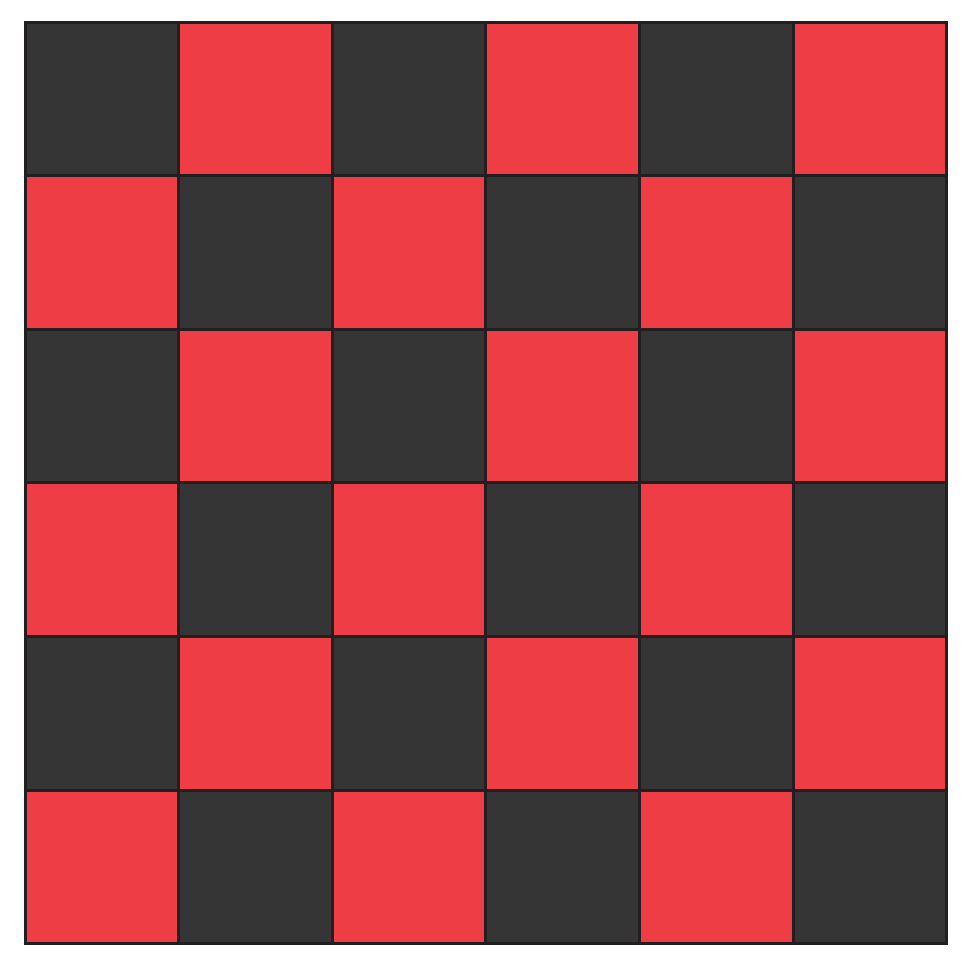
\includegraphics[width=55mm]{img/redblack.pdf}
\caption{In Red Black Gauss-Seidel iterations, the grid domain is divided in to a red and a black region. }
\label{redblack}
\end{figure}

\subsection{Restriction and Prolongation operations}

Until this moment we have not talked about the grid size $N_x$ and $N_y$. To make things as simply as possible in this report, we only allow the grid size to be a power of two.

\begin{equation}
2^M = max(N_x, N_y)
\end{equation}

Before we break down the Multigrid algorithm itself, we need a method to go from a matrix $A^M$ with resolution $N_x,N_y$ to a lower resolution matrix $A^{M-1}$ with dimensions halfed in size, i.e $N_x/2,N_y/2$. In general, we need an operation that uses a matrix $A^{M-m}$ with dimensions $\frac{N_x}{2^m}$ as an input and produces a scaled matrix $A^{M-m-1}$. This operation is called restriction. In this report we will use bilinear interpolation for downscaling a matrix.

\begin{equation}
A^{M-n-1}_{i,j} = \frac{1}{4} ( A^{M-n}_{2i,2j} + A^{M-n}_{2i + 1,2j} + A^{M-n}_{2i + 1,2j +1 }  + A^{M-n}_{2i,2j + 1} )
\label{restricteq}
\end{equation}

Figure \ref {restrict} gives a numerical example of the restriction operation seen in Equation \ref{restricteq}

\begin{figure}[ht!]
\centering
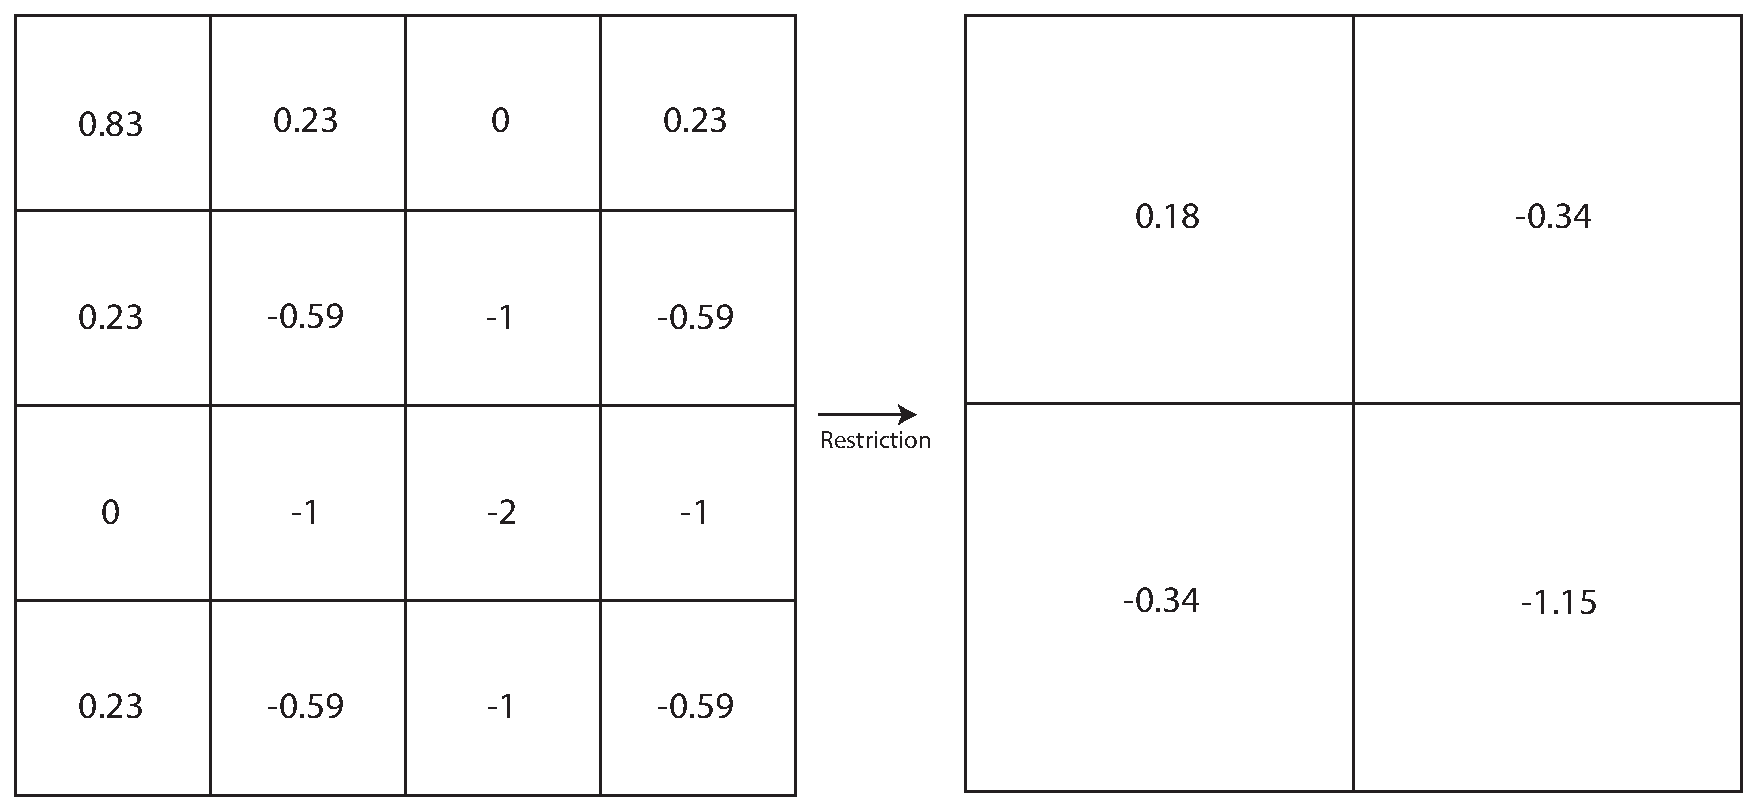
\includegraphics[width=120mm]{img/restrict.pdf}
\caption{A numerical example of the restriction operation.}
\label{restrict}
\end{figure}

To keep things simple, we also use bilinear interpolation in the prolongation operator where we do the opposite from restriction, i.e go from $A^{M-m}$ to $A^{M-m+1}$. Although using the same interpolation scheme, prolongation is a bit trickier to get right since the indices are not aligned up as perfect as in the restriction operator. Figure \ref {prolong} demonstrates why the indices are aligned slightly awkward.

\begin{figure}[ht!]
\centering
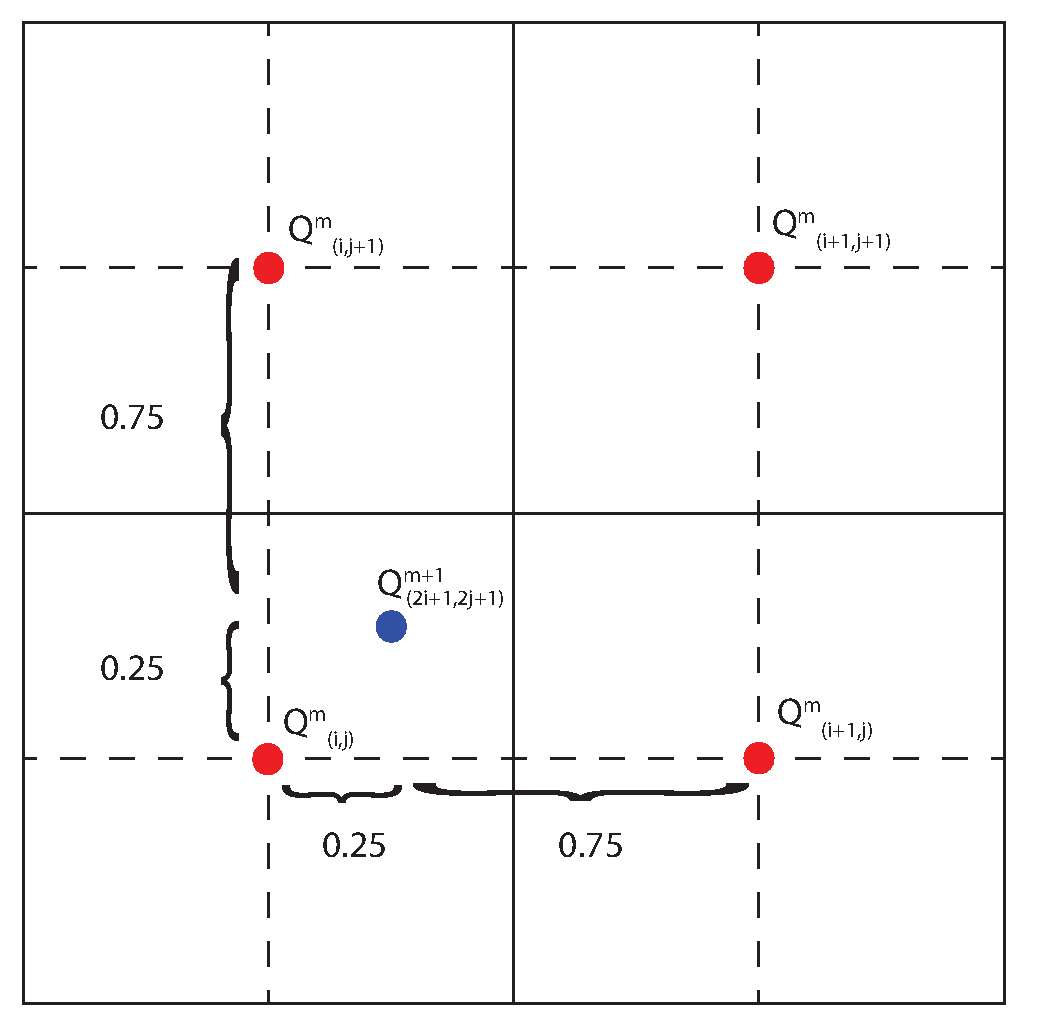
\includegraphics[width=80mm]{img/prolong.pdf}
\caption{Barycentric coordinates are used to deterimine bilinear interpolation in the prolongation operator.}
\label{prolong}
\end{figure}

To use the bilinear interpolation, we use the barycentric coordinates of each cell in $M-n$ compared to its neighboring cell in $M-n-1$ as can be seen in Figure \ref{prolong}. This gives us the following scheme for the prolongation operator:

\begin{equation}
\begin{split}
A^{M-n}_{2i,2j} &= \frac{1}{16} A^{M-n-1}_{i-1,j-1} +  \frac{3}{16} A^{M-n-1}_{i-1,j} +  \frac{3}{16} A^{M-n-1}_{i,j-1}+  \frac{9}{16} A^{M-n-1}_{i,j} \\ 
A^{M-n}_{2i + 1,2j} &= \frac{1}{16} A^{M-n-1}_{i+1,j-1} +  \frac{3}{16} A^{M-n-1}_{i,j-1} +  \frac{3}{16} A^{M-n-1}_{i+1,j}+  \frac{9}{16} A^{M-n-1}_{i,j} \\ 
A^{M-n}_{2i,2j+1} &= \frac{1}{16} A^{M-n-1}_{i-1,j+1} +  \frac{3}{16} A^{M-n-1}_{i-1,j} +  \frac{3}{16} A^{M-n-1}_{i,j+1}+  \frac{9}{16} A^{M-n-1}_{i,j} \\ 
A^{M-n}_{2i+1,2j+1} &= \frac{1}{16} A^{M-n-1}_{i+1,j+1} +  \frac{3}{16} A^{M-n-1}_{i+1,j} +  \frac{3}{16} A^{M-n-1}_{i,j+1}+  \frac{9}{16} A^{M-n-1}_{i,j} \\ 
\end{split}
\label{prolongeq}
\end{equation}

Equation \ref{prolongeq} only works if the updated cells are not on the boundary and has four neighboring cells in the lower dimension grid. If the cell is on the boundary, we use simple linear interpolation between the two cells in $A^{M-n-1}$ with weights $0.75$ and $0.25$. Before we move on to the Multigrid algorithm, there one last special case. At the four corners, we use the same value as the corners of the lower dimension grid since there is nothing nearby to interpolate from.

\subsection{The Multigrid method}

One problem with iterative solvers of linear systems of equations is that information propgates very slowly. In Equation \ref{jacobi}, only neighboring cells are part of this expression and therefore information only moves one cell per iteration step. This means that the larger the grid size $N_x, N_y$ is, the longer it takes to reach convergence. We are not guaranteed that our velocity field is divergence-free if the solution to $Ap=b$ does not convergence. However, choosing a low resolution grid introduces other non-wanted artifacts. An approach with high accuracy and fast convergence is desirable. The multigrid method tries to satisfy this where the main idea is to solve the linear system of equations in different resolutions and then use restriction and prolongations operations to transfer the answer from one resolution to another. There are different options on how to reach convergence and in this report we will focus on \emph{Full Cycle} and \emph{V-Cycle}. FIgure \ref{multigrid} demonstrates the difference between the two. Note that the Full Cycle uses incremental V-Cycles, something we can take advantage of when implementing the Full Cycle.

\begin{figure}[ht!]
\centering
\begin{subfigure}[]{0.3\textwidth}
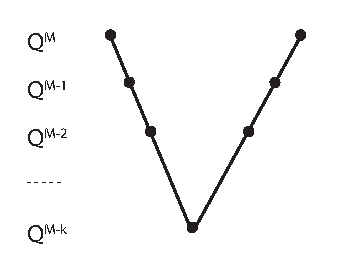
\includegraphics[height=41mm]{img/vcycle.pdf}
\end{subfigure}
\begin{subfigure}[]{0.3\textwidth}
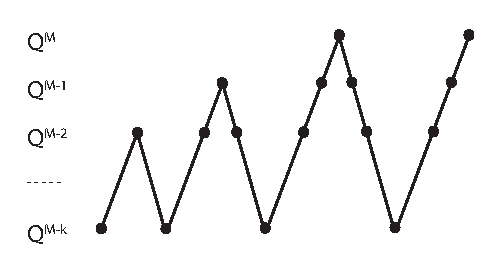
\includegraphics[height=41mm]{img/fullcycle.pdf}
\end{subfigure}
\caption{The two different multigrid schemes presented in this report, \emph{V-Cycle (left)} and \emph{Full cycle (right)}.}
\label{multigrid}
\end{figure}


Using restriction and prolongation on the pressure grid in the V-cycle acts as a low pass filter and this an unwanted effect. Instead of moving the pressure solution from one resolution to another, we will use restriction and prolongation on the residual $r^{M-n} = b^{M-n} - A^{M-n}p^{M-n}$. Instead of solving $Ap = b$ in each resolution, we solve $Ap = r$. To update the pressure of level $M-n$ we use the linear combination of $p^{M-n}$ and $prolong(p^{M-n-1})$.

\begin{equation}
p^{M-n}_{n+1} = p^{M-n}_n + prolong(p^{M-n-1})
\end{equation}

\begin{equation}
r^{M-n} = b^{M-n} - A^{M-n} p^{M-n}_n 
\end{equation}

Equation \ref{multigridsplit} explains why using a linear combination of two different resolutions (where the lower resolution one have had the prolongation operator applied to it) work in the V-cycle update.

\begin{equation}
\begin{split}
A^{M-n} p^{M-n}_{n+1} &= b^{M-n} \\
A^{M-n} (p^{M-n}_n + prolong(p^{M-n-1})) &= b^{M-n} \\
A^{M-n} prolong(p^{M-n-1}) +  \underbrace{ A^{M-n} p^{M-n}_n -  b^{M-n} }_\text{$-r^{M-n}$} &= 0 \\
A^{M-n} prolong(p^{M-n-1})  &= r^{M-n}
\end{split}
\label{multigridsplit}
\end{equation}

If $M$ is the inital resolution number for the grid, we can specify a lower minimum resolution number $K$. Solving the pressure equations for grids with dimension sizes small as $1$ and $2$ makes little sense since we can't even specify the pressure equations. 

\begin{algorithm}
\caption{Multigrid method}
\begin{algorithmic}[1]
\FOR{$m = M - 1$ down to $K$}
\STATE $\phi^m$ = restrict($\phi^{m+1}$)
\STATE $\phi^m_s$ = restrict($\phi^{m+1}_s$)
\ENDFOR

\FOR{$m = M$ down to $K$}
\STATE Build sparse matrix $A^m$
\ENDFOR

\STATE Build right hand side $b$
\STATE Initial guess $p^M = 0$

\FOR{i = 1 to $N_{\text{Full cycle}}$}
\STATE Full cycle
\ENDFOR

\FOR{i = 1 to $N_{\text{V cycle}}$}
\STATE V cycle(M)
\ENDFOR

\end{algorithmic}
\label{multigridalgorithm}
\end{algorithm}


\begin{algorithm}
\caption{V cycle(m)}
\begin{algorithmic}[1]

\FOR{i = 1 to $N_{\text{sweep}}$}
\STATE Gauss-Seidel to solve $A^mp^m = r^m$
\ENDFOR

\STATE $r^m = r^m - A^mp^m$
\STATE $r^{m-1} = restrict(r^m)$
\STATE $p^{m-1} = 0$
\STATE V cycle(m-1)
\STATE $p^m = p^m + prolong(p^{m-1})$

\FOR{i = 1 to $N_{\text{sweep}}$}
\STATE Gauss-Seidel to solve $A^mp^m = r^m$
\ENDFOR

\end{algorithmic}
\label{multigridalgorithm}
\end{algorithm}

In Algorithms \ref{vcyclealgorithm}, \ref{vcyclealgorithm} and \ref{fullcyclealgorithm}, we only use the restriction operators on the surface tracking level sets and the residual. The prolongation operator is only used on the pressure grids. 

\begin{algorithm}
\caption{Full cycle()}
\begin{algorithmic}[1]

\STATE $p^{tmp} = p^M$
\FOR{m = K to M}
\IF{$m \neq K$}
\STATE $p^m = prolong(p^{m-1})$
\ENDIF
\STATE V cycle(m)

\ENDFOR

\STATE $p^M = p^{tmp} + p^M$

\end{algorithmic}
\label{fullcyclealgorithm}
\end{algorithm}

We know have all the components we need to solve the pressure equations and make sure the velocity field is divergence free. As far as the multigrid method goes, there are three variables we can tweak for performance and convergence rate. The first one is $N_{sweep}$ that determines how many iterations of Gauss-Seidel are performed in each resolution. The other two, $N_{\text{Full cycle}}$ and $N_\text{V cycle}$, changes the number of step for each cycle method. In theory the Full cycle is faster but in practise with implementations, all the restriction and prolongation operations can be expensive. In general, the larger $N_{sweep}$ is, the smaller can $N_{\text{Full cycle}}$ and $N_\text{V cycle}$ be and vice verse. The most optimal choice of parameters is situational and how to automatically detect the different scenarios is beyond this report. 


\newpage
\section{Results}
A single threaded test application was programmed in C++ to evaluate the FLIP water simulation with multigrid as pressure solving method. No external libraries other than the C++ standard library was used in the simulation. The graphics library OpenGL was used to display the simulation where each particle in the FLIP simulation is represented as a blue quad. The simulation generated data for display $24$ times per second.
\newline
\newline
The resolution of the grid in the test application was set to $128$ for both $N_x$ and $N_y$. The size of each side in the grid was set to $1 m$ which gives each cells a width of $\Delta x = 0.0078$. As can be seen in the Figure \ref{initialshapae}, the initial shape of the simulation is a half sphere. The solid wall boundaries are placed at the grid boundaries with one grid cell as the width. No extra solids to collide against were used. Parts of the simulation can be seen in Figure \ref{simresult}. More images of the multigrid simulation can be found in Appendix A. 

\begin{figure}[ht!]
\centering

\begin{subfigure}[]{0.3\textwidth}
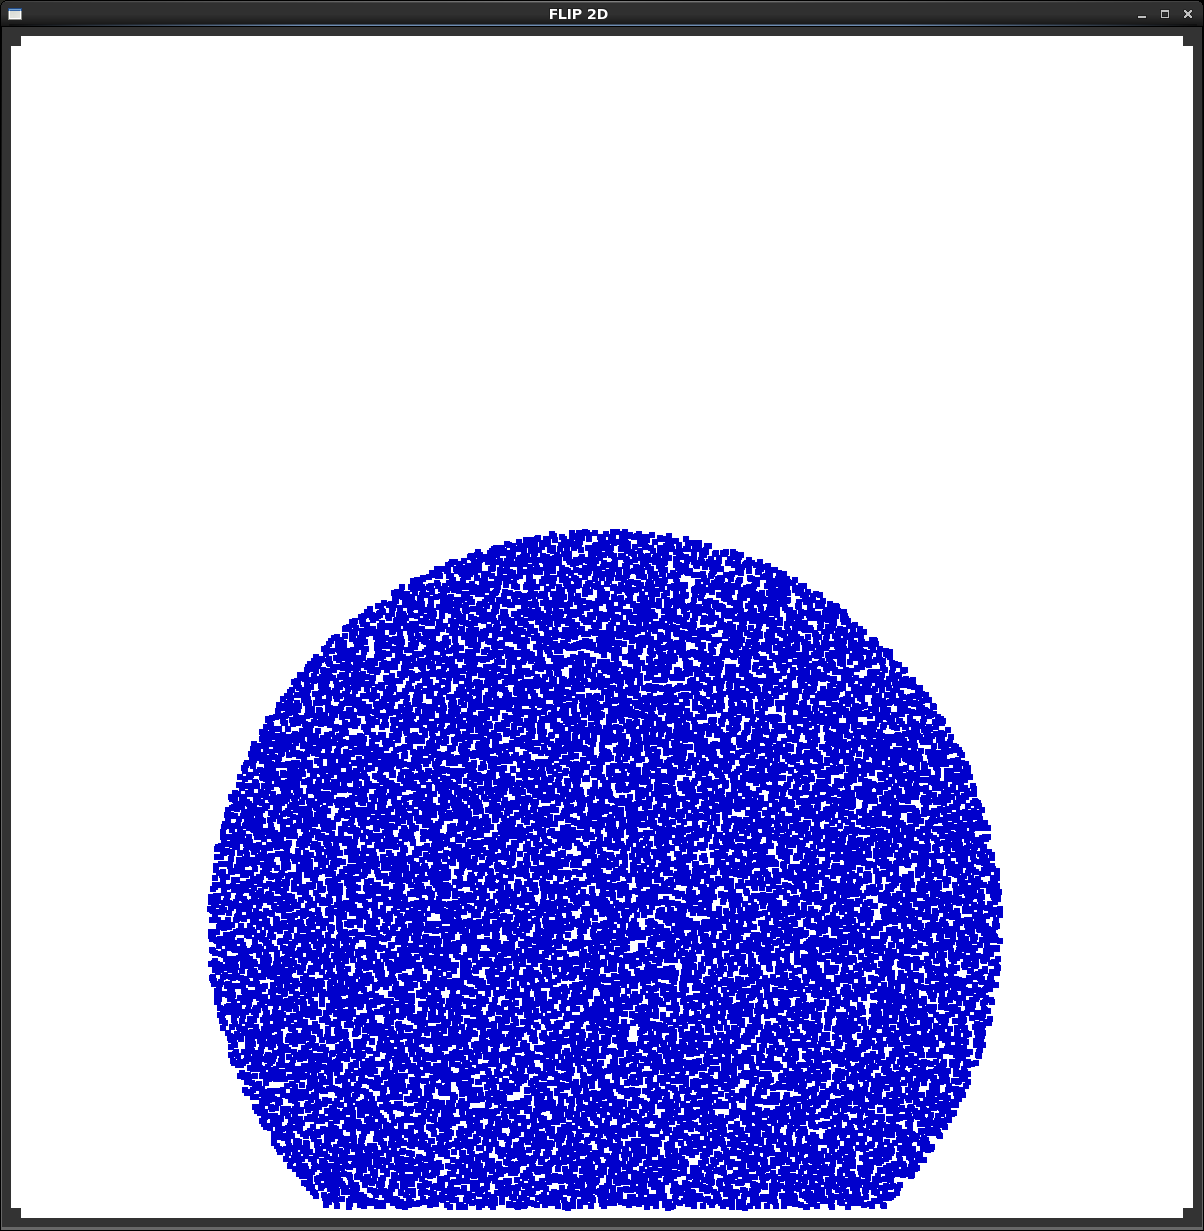
\includegraphics[height=45mm]{png/multigrid0.png}
\caption{Frame 0.}
\label{initialshapae}

\end{subfigure}
\begin{subfigure}[]{0.3\textwidth}
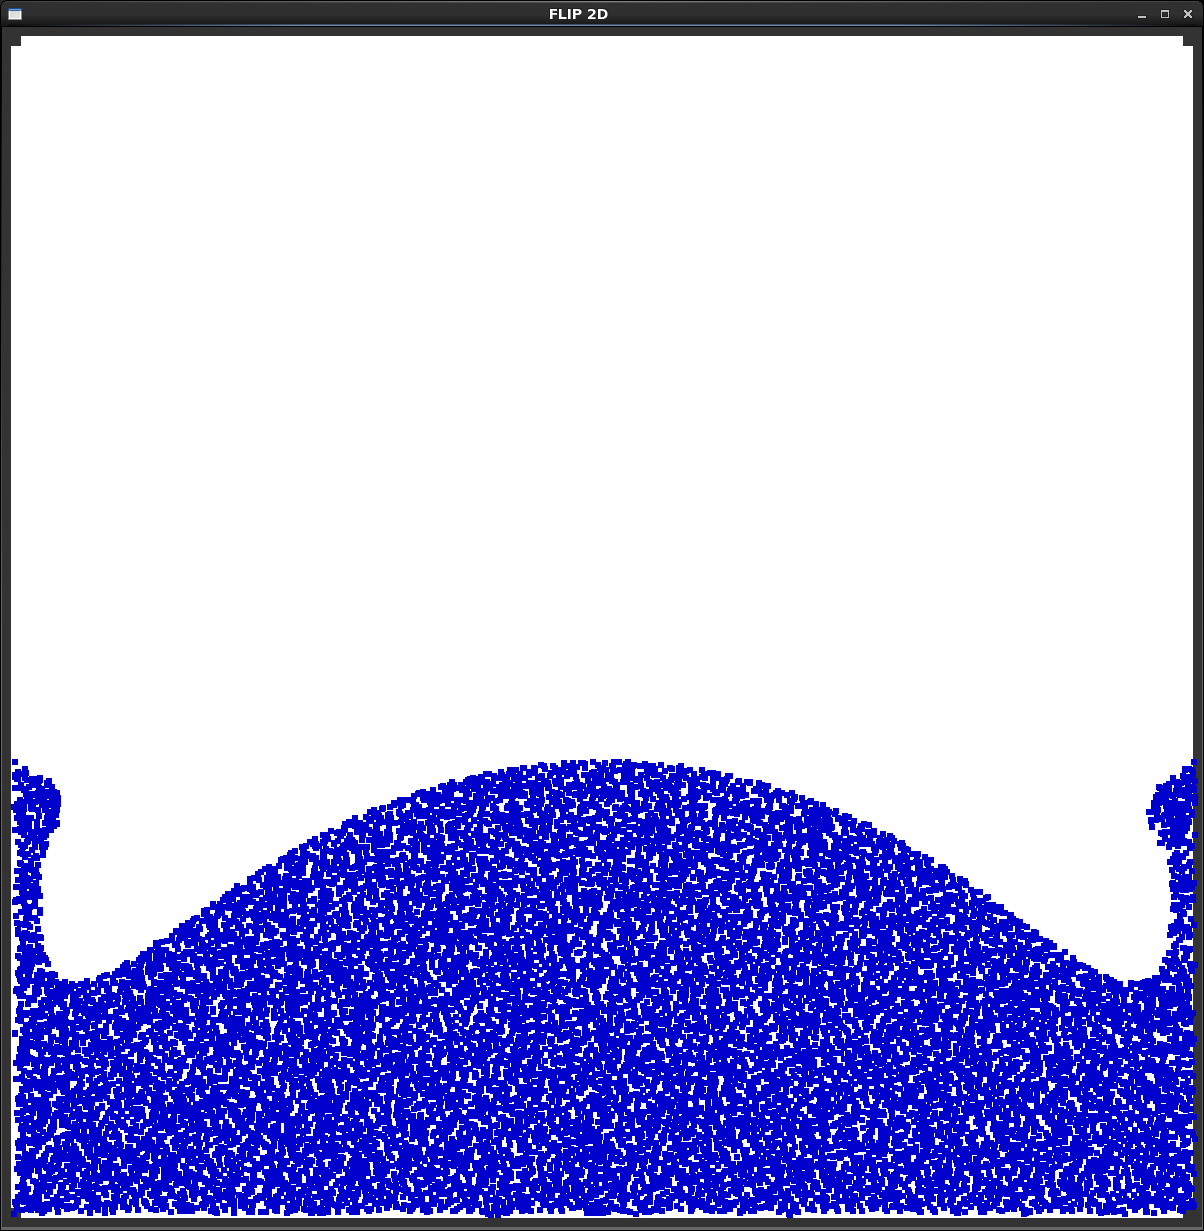
\includegraphics[height=45mm]{png/multigrid1.png}
\caption{Frame 15.}
\end{subfigure}

\begin{subfigure}[]{0.3\textwidth}
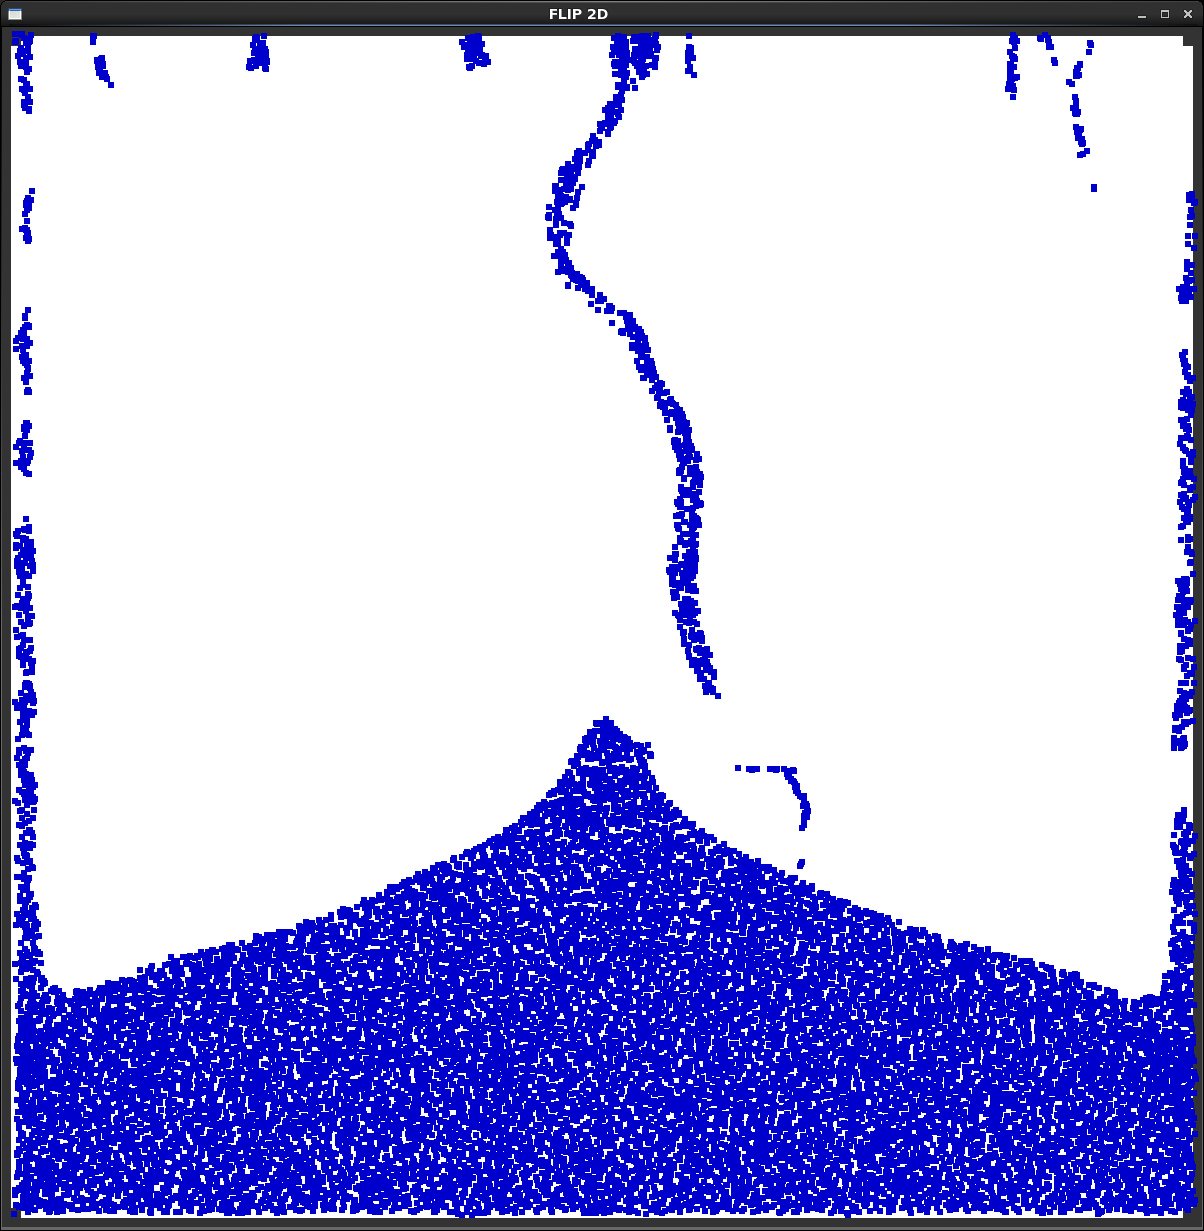
\includegraphics[height=45mm]{png/multigrid4.png}
\caption{Frame 60.}
\end{subfigure}

\caption{Results of the multigrid simulation.}
\label{simresult}
\end{figure}
\noindent
The multigrid parameters used in Figure \ref{simresult} are $N_{sweep} = 10$ and $N_{\text{Full cycle}} = N_\text{V cycle} = 4$. Figure \ref{lowvshigh} shows the difference between using a low number of cycles vs a high number of cycles. When $N_{\text{Full cycle}}$ and $N_\text{V cycle}$ are set to lower values, we see volume loss artifacts.

\begin{figure}[ht!]
\centering
\begin{subfigure}[]{0.3\textwidth}
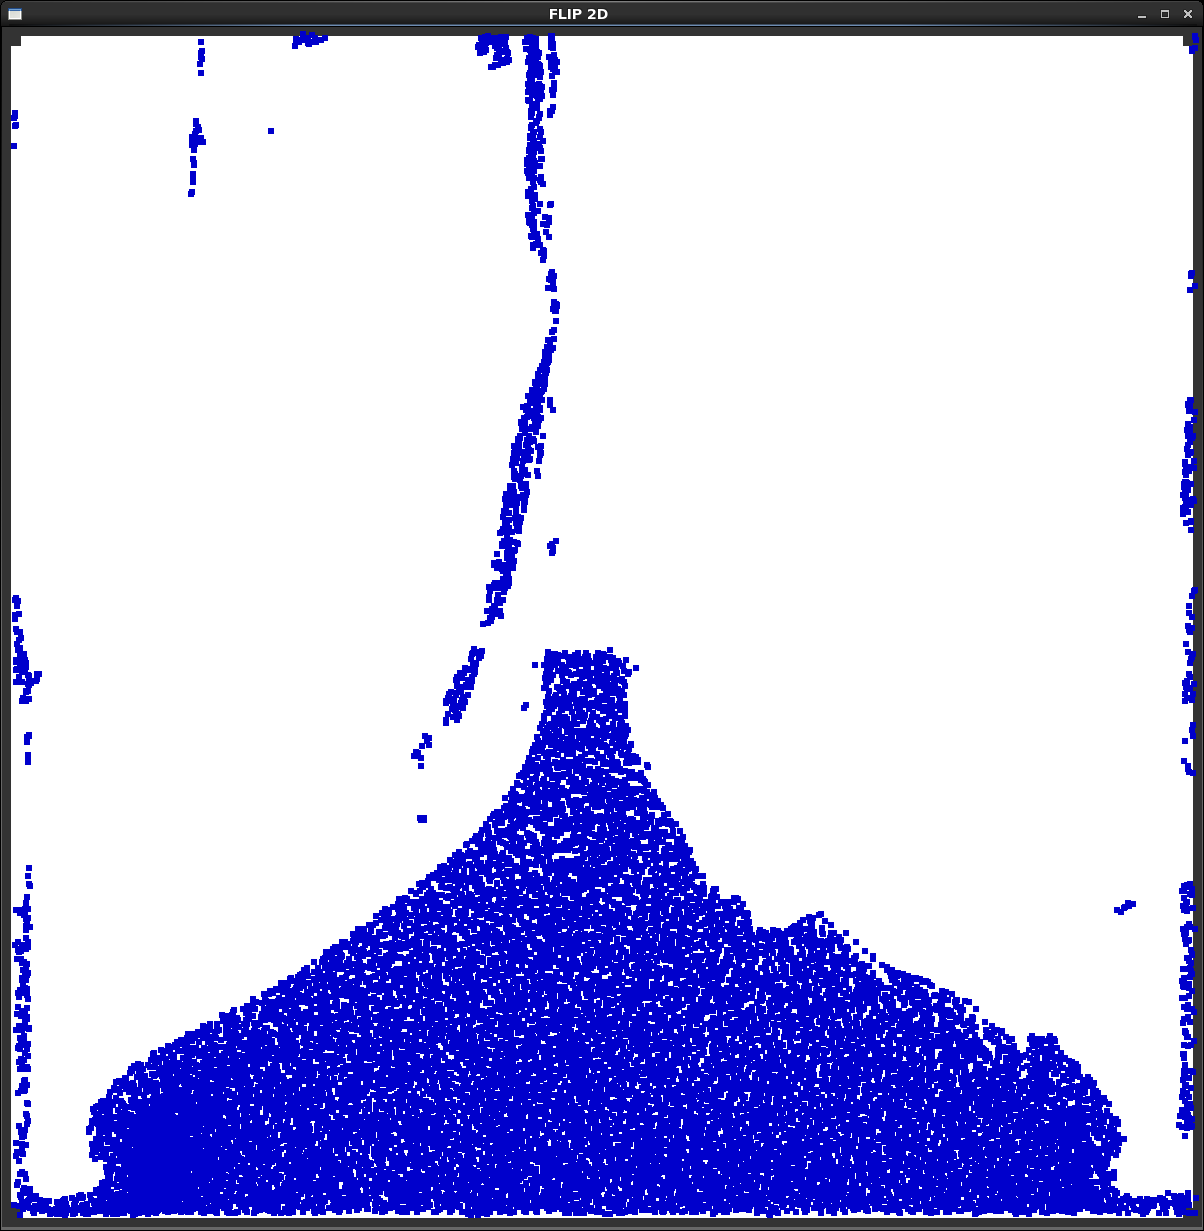
\includegraphics[height=45mm]{png/multigridN1.png}
\caption{$N_{\text{\{Full,V\} cycle}} = 1$.}
\end{subfigure}
\begin{subfigure}[]{0.3\textwidth}
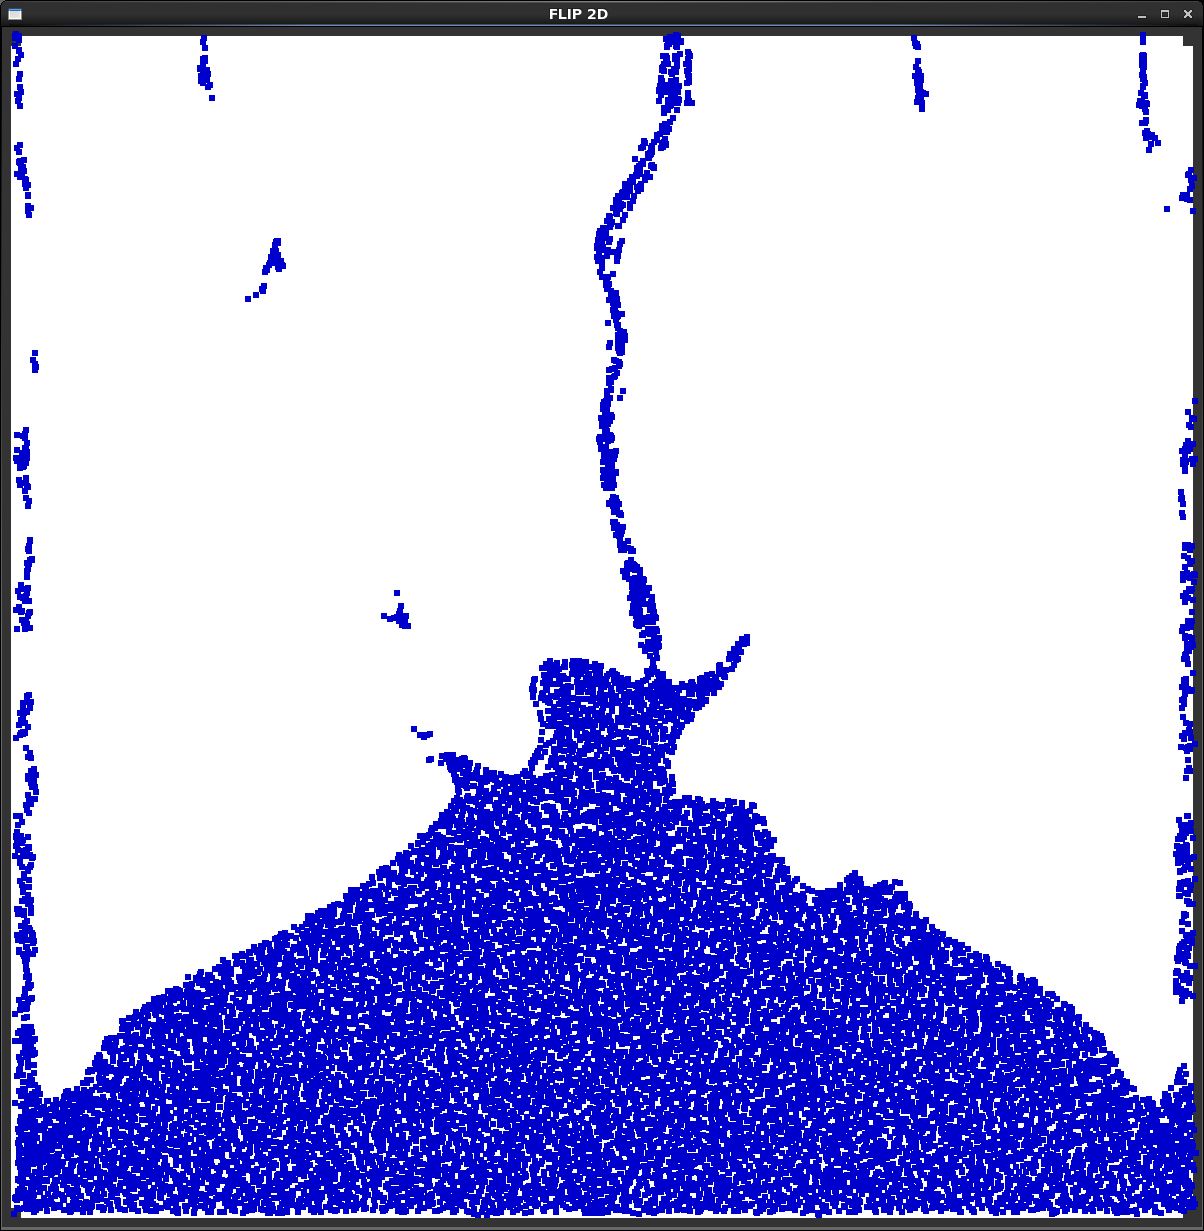
\includegraphics[height=45mm]{png/multigridN8.png}
\caption{$N_{\text{\{Full,V\} cycle}} = 8$.}
\end{subfigure}
\caption{}
\label{lowvshigh}
\end{figure}
\noindent
A preconditioned conjugate gradient, PCG, pressure solver with incomplete cholesky factorization as the preconditioner was also implemented in the test application to test correctness. For information about the implementation, one can find a detailed explanation in \cite{bridson}. A quick comparison between the multigrid method (with both cycles to be run 4 times) vs PCG can be seen in Figure \ref{pcgvsmulti}. Although different pressure solving methods, they produce solutions that look similar. Images of the full PCG simulation can be found in Appendix B. 

\begin{figure}[ht!]
\centering
\begin{subfigure}[]{0.3\textwidth}
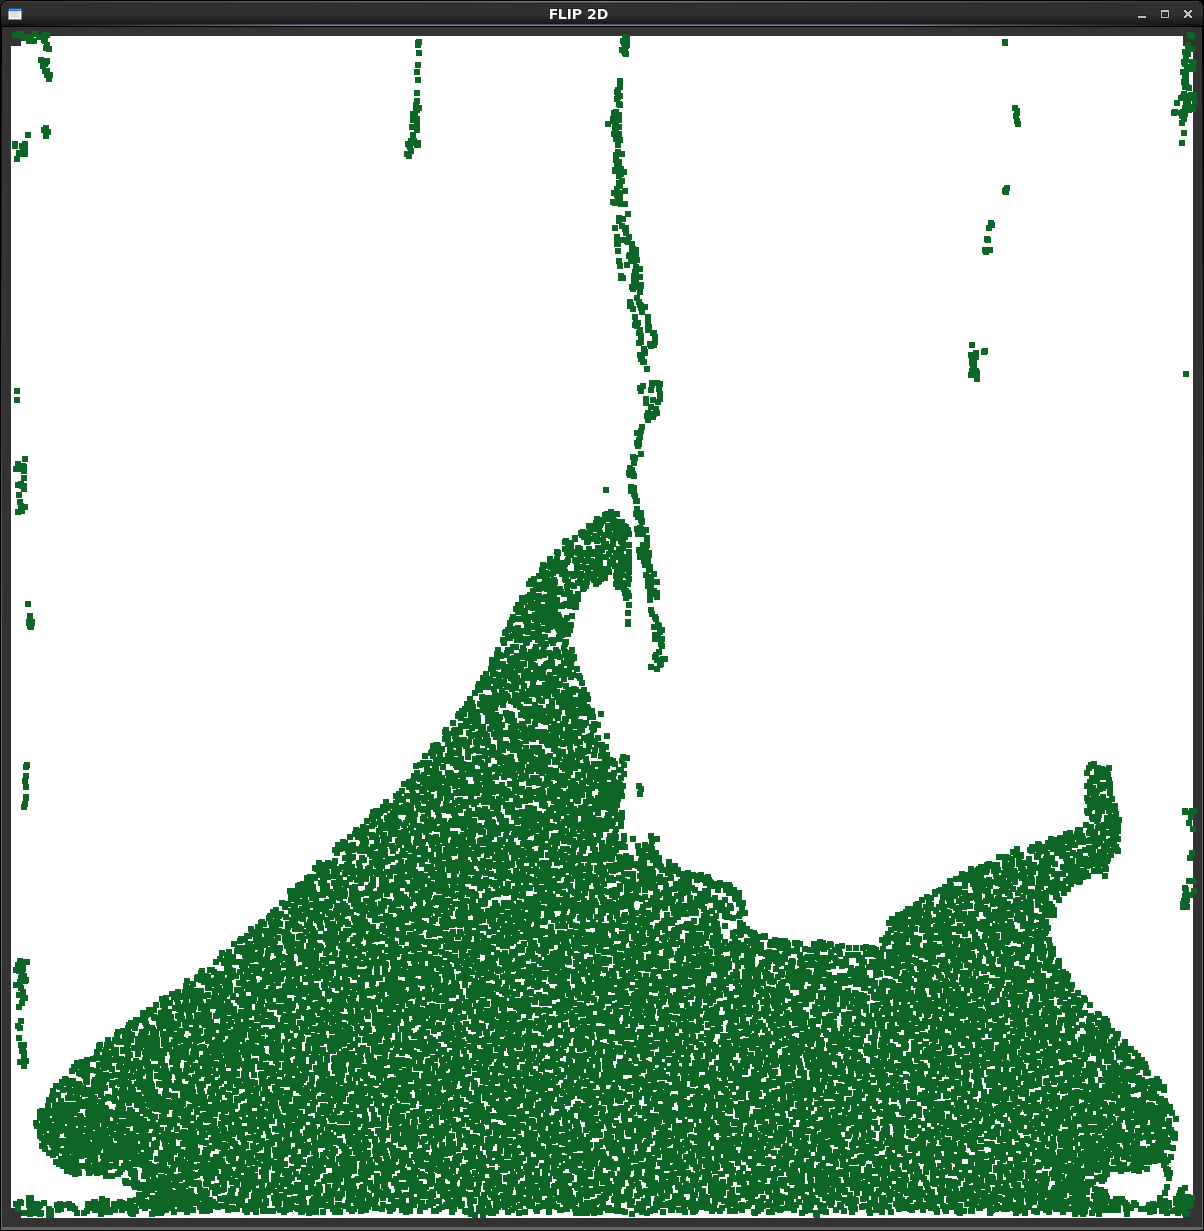
\includegraphics[height=45mm]{png/pcg5.png}
\caption{PCG.}
\end{subfigure}
\begin{subfigure}[]{0.3\textwidth}
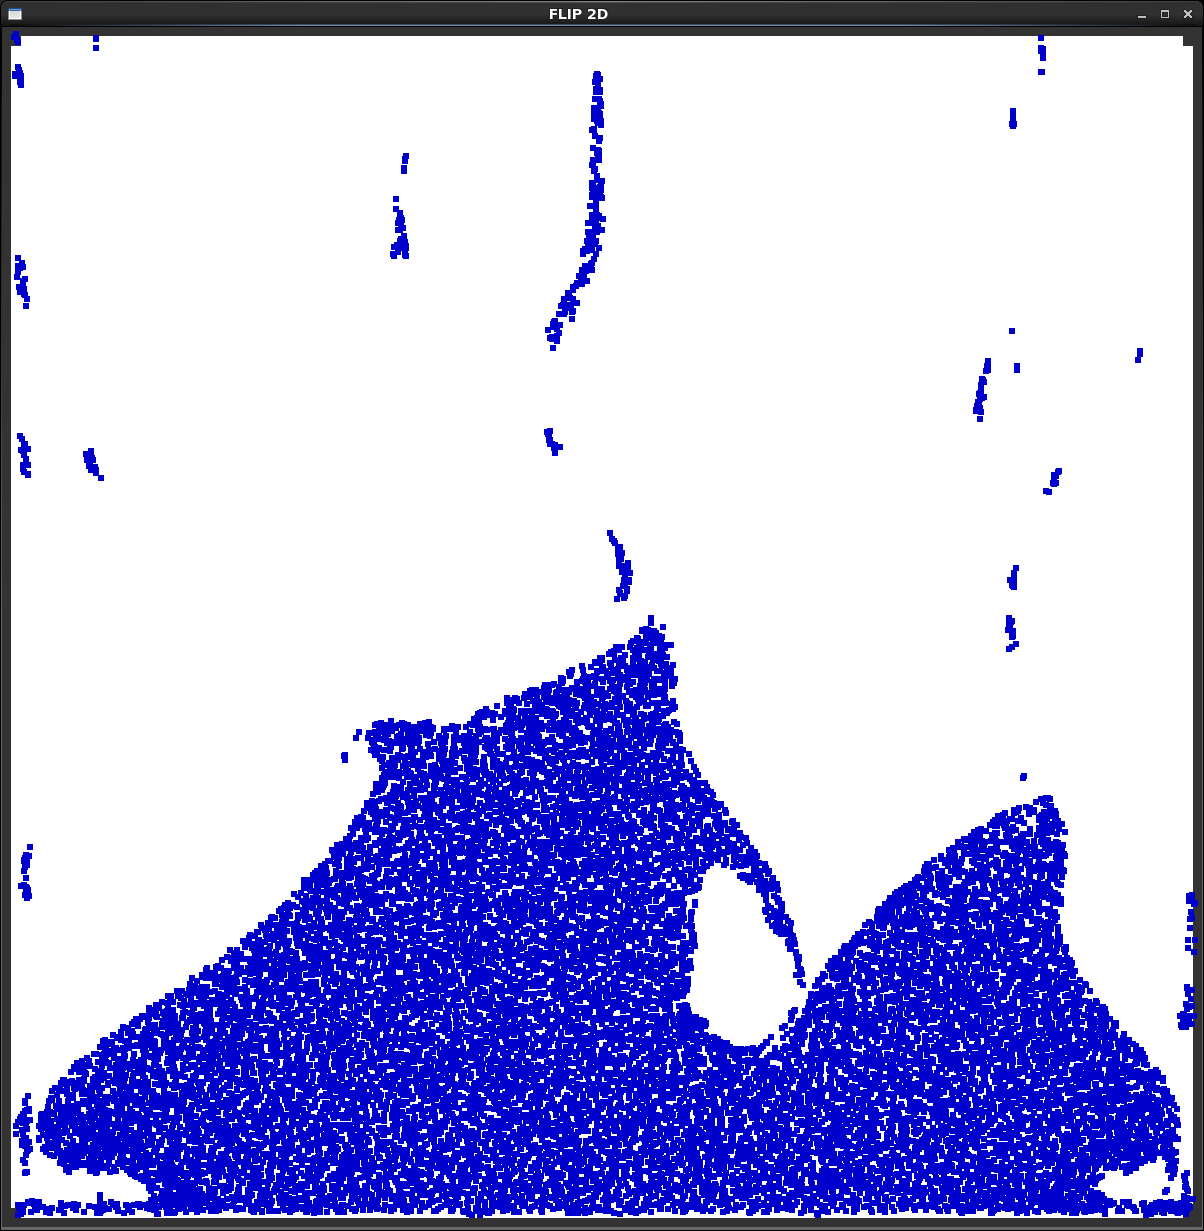
\includegraphics[height=45mm]{png/multigrid5.png}
\caption{Multigrid.}
\end{subfigure}
\caption{A comparison at frame 70 between the PCG method (green) and the multigrid method (blue).}
\label{pcgvsmulti}
\end{figure}


\newpage
\section{Discussion}
\subsection{Improving Boundary Conditions}
In chapter 5 we assumed that the boundary conditions were always aligned perfectly with the grid cells. We also assumed that the velocity of all solids were zero. If we would allow solids to have a velocity $\vec{u^{solid}}$, Equation \ref{solidveleq} has to be changed to

\begin{equation}
u^{solid}_{i+1/2,j}  = {u^*}_{i+1/2,j} - \frac{\Delta t }{\rho}\frac{p_{i+1,j} - p_{i,j}}{\Delta x}
\end{equation}

%\noident
The more complicated case when setting up the pressure equations is when a cell is only partially covered with solid or air. Figure \ref{boundarycases} shows two different cases, one that our simple approach covers very well and one that would lead to rectangular artifacts.

\begin{figure}[ht!]
\centering
\begin{subfigure}[]{}
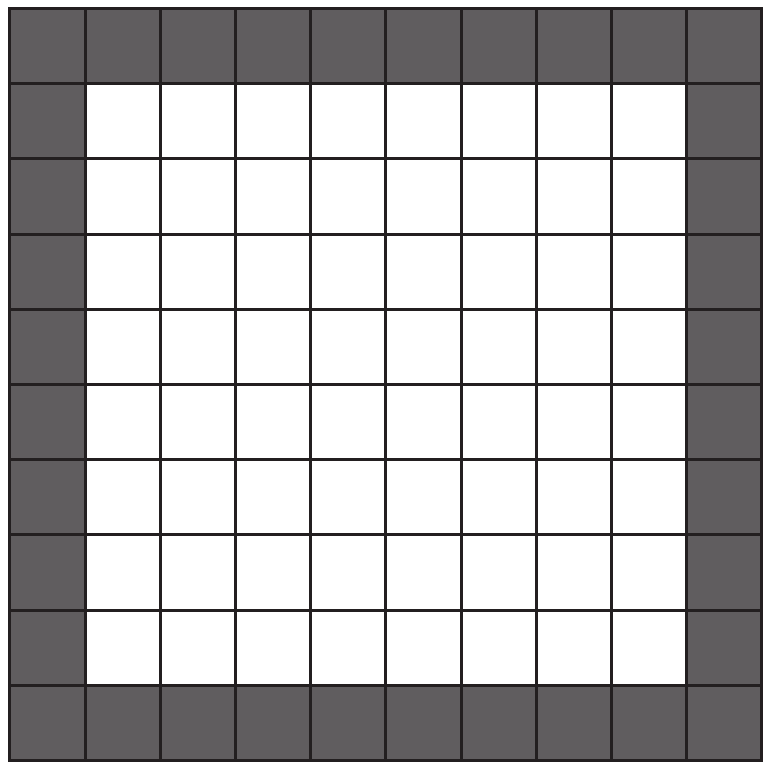
\includegraphics[height=41mm]{img/boundary1.pdf}
\end{subfigure}
\begin{subfigure}[]{}
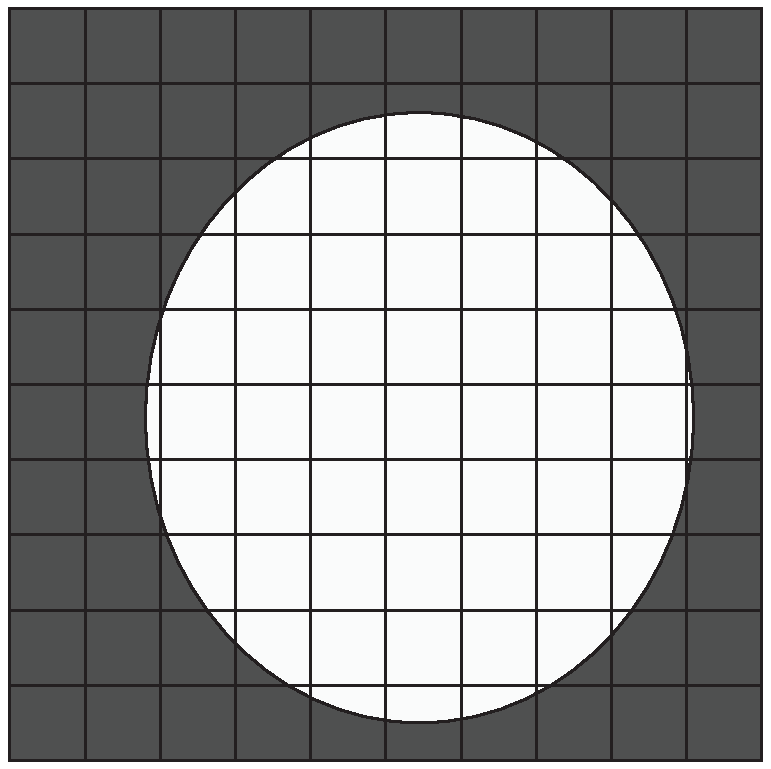
\includegraphics[height=41mm]{img/boundary2.pdf}
\end{subfigure}
\caption{Regular (a) vs irregular (b) solid boundaries.}
\label{boundarycases}
\end{figure}

Batty et al \cite{batty} presented a way to deal with irregular boundary geometry. It would be interesting to apply their ideas to the fluid multigrid solver in this thesis. When setting up the pressure equations, we would need a way to find out how much of a cell is covered by fluid. Even more specific, how much of the area nearby an edge is covered by fluid? The only change we would have to make would be in Equation \ref{pressureeq}. If $m$ is the previously mentioned fluid cover function ($0 \leq m \leq 1$), our linear system of equations need to satisfy the following:

\begin{equation}
\begin{split}
(m_{i-1/2,j} + m_{i+1/2,j} + m_{i,j-1/2} + m_{i,j+1/2})p_{i,j} - \\ 
m_{i-1/2,j} p_{i-1,j} - 
m_{i+1/2,j}p_{i+1,j} & - \\
m_{i,j-1/2}p_{i,j-1} - 
m_{i,j+1/2}p_{i,j+1} = \\ 
-\frac{\rho \Delta x}{\Delta t}(m_{i+1/2,j}{u^*}_{i+1/2,j} - m_{i-1/2,j}{u^*}_{i-1/2,j} + \\
m_{i,j+1/2}{v^*}_{i,j+1/2} - m_{i,j-1/2} {v^*}_{i,j-1/2})
\end{split}
\label{pressureeqvariational}
\end{equation}

\subsection{Advecting the Level Set}

We are constantly redefining the surface each step based on the position of the particles. This can lead to a noisy surface tracking. Another option that would be interesting to try would be to create a smooth level set once and then advect the level set. The free surface, where $\phi = 0$ should be advected with the fluid velocity and we need to solve Equation \ref{advectlevelset}.

\begin{equation}
\frac{\partial \phi}{\partial t} + \nabla \phi \cdot \vec{u} = 0
\label{advectlevelset}
\end{equation}

Fedkiw and Osher \cite{osher} introduced high-order methods for solving Equation \ref{advectlevelset}. If we advect both the level set and all particles every substep there will be cases where particles exists in regions where $\phi > 0$. What to do with those particles is not clear. One option would be to only advect the escaped particles in the extrapolated velocity field and not let them affect the pressure solve.

\subsection{Parallel implementation}

Solving for pressure is the largest and the most computational expensive part of the FLIP algorithm. Most fluid simulators have traditionally been using a preconditioned conjugate gradient pressure solver. A very popular preconditioner to use is the Incomplete Cholesky Factorization. Although making the conjugate gradient method to converge faster, this preconditioner cn not be run in parallell which is unfortunate since one has to apply the preconditioner before every conjugate gradient step. The multigrid approach has the big advantage that every step is easy to port from a serial implementation to a parallel one. Given a grid size of $N_x$ and $N_y$, one can simply divide the grid into subregions proportional to the number of cores present on the arcitechure performing the computations. One of the benefits using the Red and Black Gauss-Seidel iteration scheme presented in Chapter 5 is that it does not matter in which order the subregions are updated in an iteration step since we are guaranteed that all neighboring cells had their values updated in previous step. The restriction and prolongation operators are also easy to perform in parallel since there are no read/write conflicts and once again the grid can be divided into subregions for each core available. Other trivial steps to run in parallel out of the items presented in the outline of the algorithm in Chapter 2 are:

\begin{enumerate}
\item Mark cells fluid
\item Apply external forces to grid
\item Create Level Set
\item Tranfser grid velocities to particles
\item Advect particles
\end{enumerate}

Transfering the particle velocities to the grid is harder to run in parallel because of the fact that two particles could potentially be writing to the same velocity in the grid at the same time and therefore introduce a write condition. This motivates us to use a special data structure for particles, storing them in different banks depending on their spatial position. Similar to the Red and Black Gauss-Seidel, we only update regions in parallel that are not neighbors and we can therefore assume that inside a thread there will never be a write condition.
\newline
\newline
Reinitializing the level set and extrapolating velocites outside of the fluid region are also a bit more complicated since these steps are both using the fast sweeping method. Jeong et al\cite{jeong}  explains an algorithm that solves the Eiokonal equation in parallel using a fast sweeping approach. Similar method can be used to extrapolate the velocities as well.


%\newpage
%\section{Conclusion}

\newpage
\begin{thebibliography}{9}
\addcontentsline{toc}{section}{References}

\bibitem{bridson}
  R. Bridson,
  \emph{Fluid Simulations for Computer Graphics.}
  1st Edition,
  2008.

\bibitem{zhu}
  Y. Zhu and R. Bridson,
  \emph{Animating Sand as a Fluid.}
  2005.

\bibitem{mueller}
  M. Mueller
  \emph{A Multigrid Fluid Pressure Solver Handling Separating Solid Boundary Conditions.}
  2011.

\bibitem{zhao}
  H. Zhao, 
  \emph{A Fast Sweeping Method for Eikonal Equation.}
  2005.

\bibitem{stam}
  J. Stam
  \emph{Stable Fluids.}
  1999.

\bibitem{fosterfed}
  N. Foster and R. Fedkiw
  \emph{Practical Animation of Liquids.}
  2001.

\bibitem{batty}
  C. Batty, F.Bertails and R. Bridson
  \emph{A Fast Variational Framework for Accurate Solid-Fluid Coupling}
  2007.

\bibitem{enright}
  D. Enright, S. Marschner and R. Fedkiw
  \emph{Animation and Rendering of Complex Water Surfaces.}
  2002.

\bibitem{harlow}
  F. H. Harlow 
  \emph{The Particle-in-Cell Method for Numerical Solution of Problems in Fluid Dynamics.}
  1963.

\bibitem{osher}
  S. Osher and R. Fedkiw
  \emph{Level Set Methods and Dynamic Implicit Surfaces.}
  2002.

\bibitem{chorin}
  A.J Chorin
  \emph{Numerical Solution to the Navier Stokes equations}
  1968.

\bibitem{sph}
 J.J Monaghan
 \emph{Smoothed particle hydrodynamocs.}
 1992.

\bibitem{desbrun}
  M. Desbrun and M.P Cani
  \emph {Smoothed particles: A new paradigm for animating highly deformable bodies.}
  1996.

\bibitem{metaxas}
  N. Foster and D. Metaxas
  \emph{Realistic animation of liquids.}
  1996.

\bibitem{jeong}
  W. K Jeong and T. Whitaker
  \emph{A fast eikonal equation solver for parallel systems.}
  2007.

\end{thebibliography}


\section*{Appendix A: Multigrid Simulation}
\addcontentsline{toc}{section}{Appendix A: Multigrid Pressure Solver Simulation}
\begin{figure}[ht!]
\centering
\begin{subfigure}[]{}
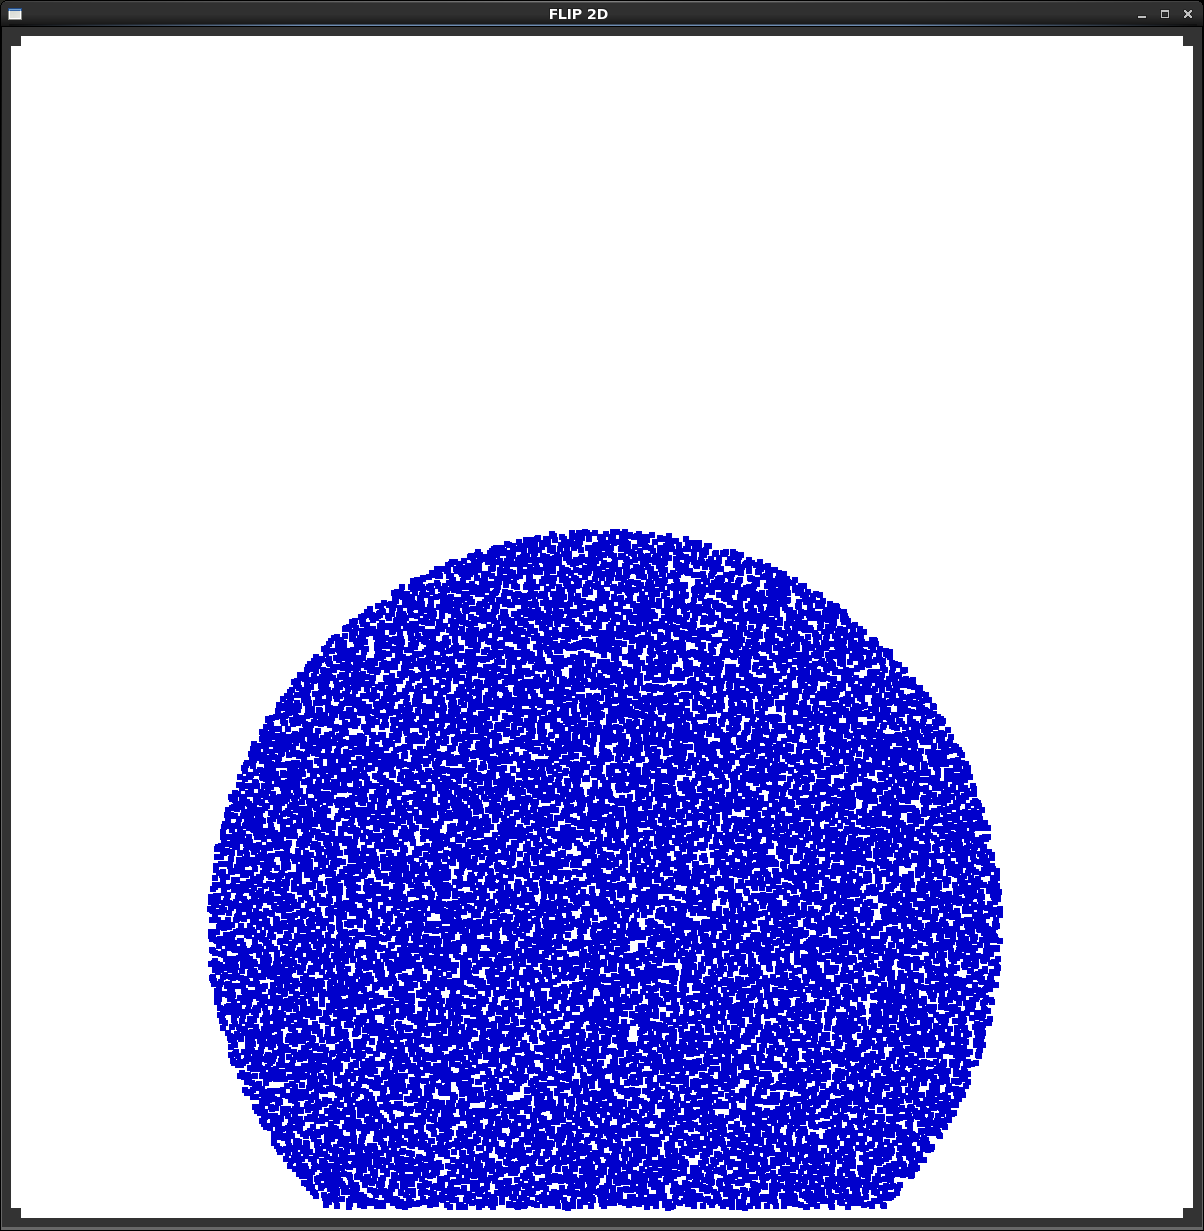
\includegraphics[height=35mm]{png/multigrid0.png}
\end{subfigure}
\begin{subfigure}[]{}
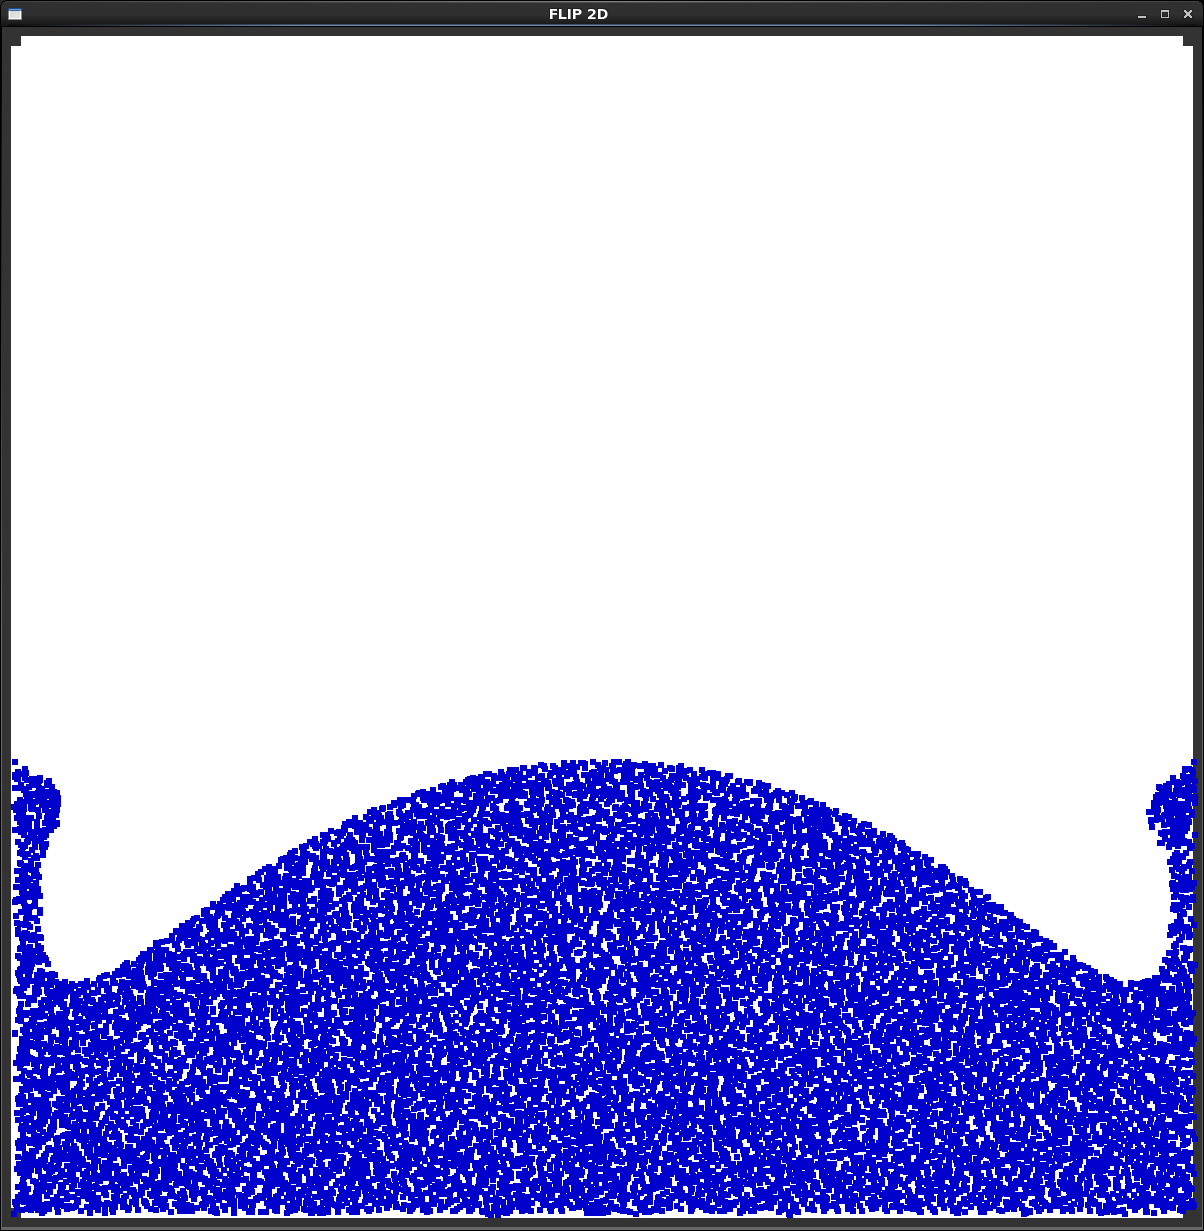
\includegraphics[height=35mm]{png/multigrid1.png}
\end{subfigure}
\begin{subfigure}[]{}
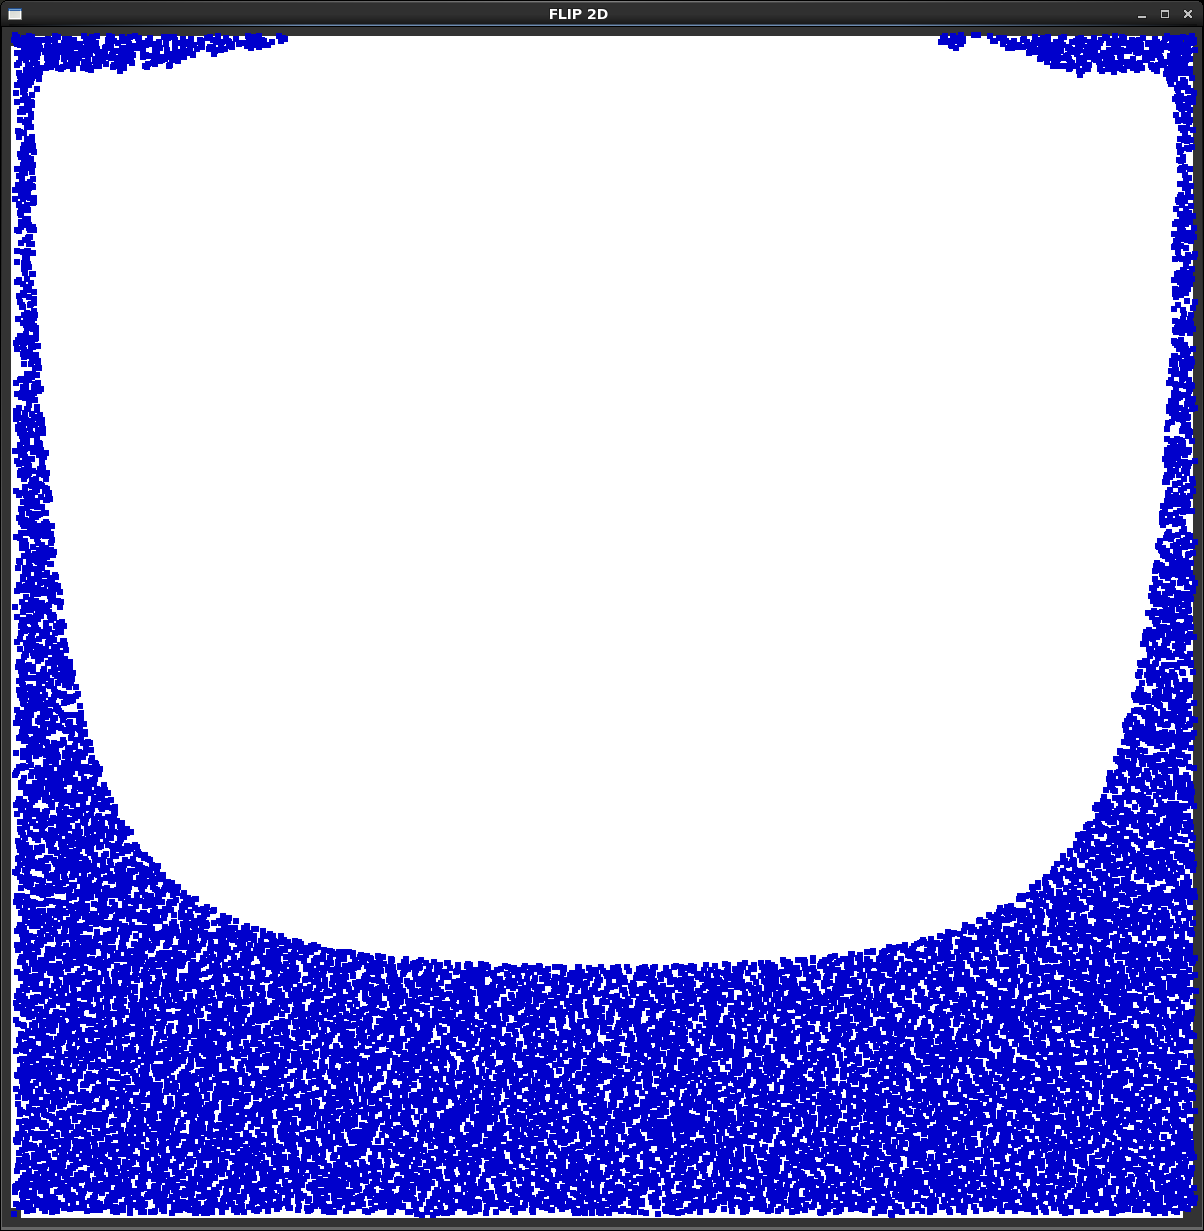
\includegraphics[height=35mm]{png/multigrid2.png}
\end{subfigure}
\begin{subfigure}[]{}
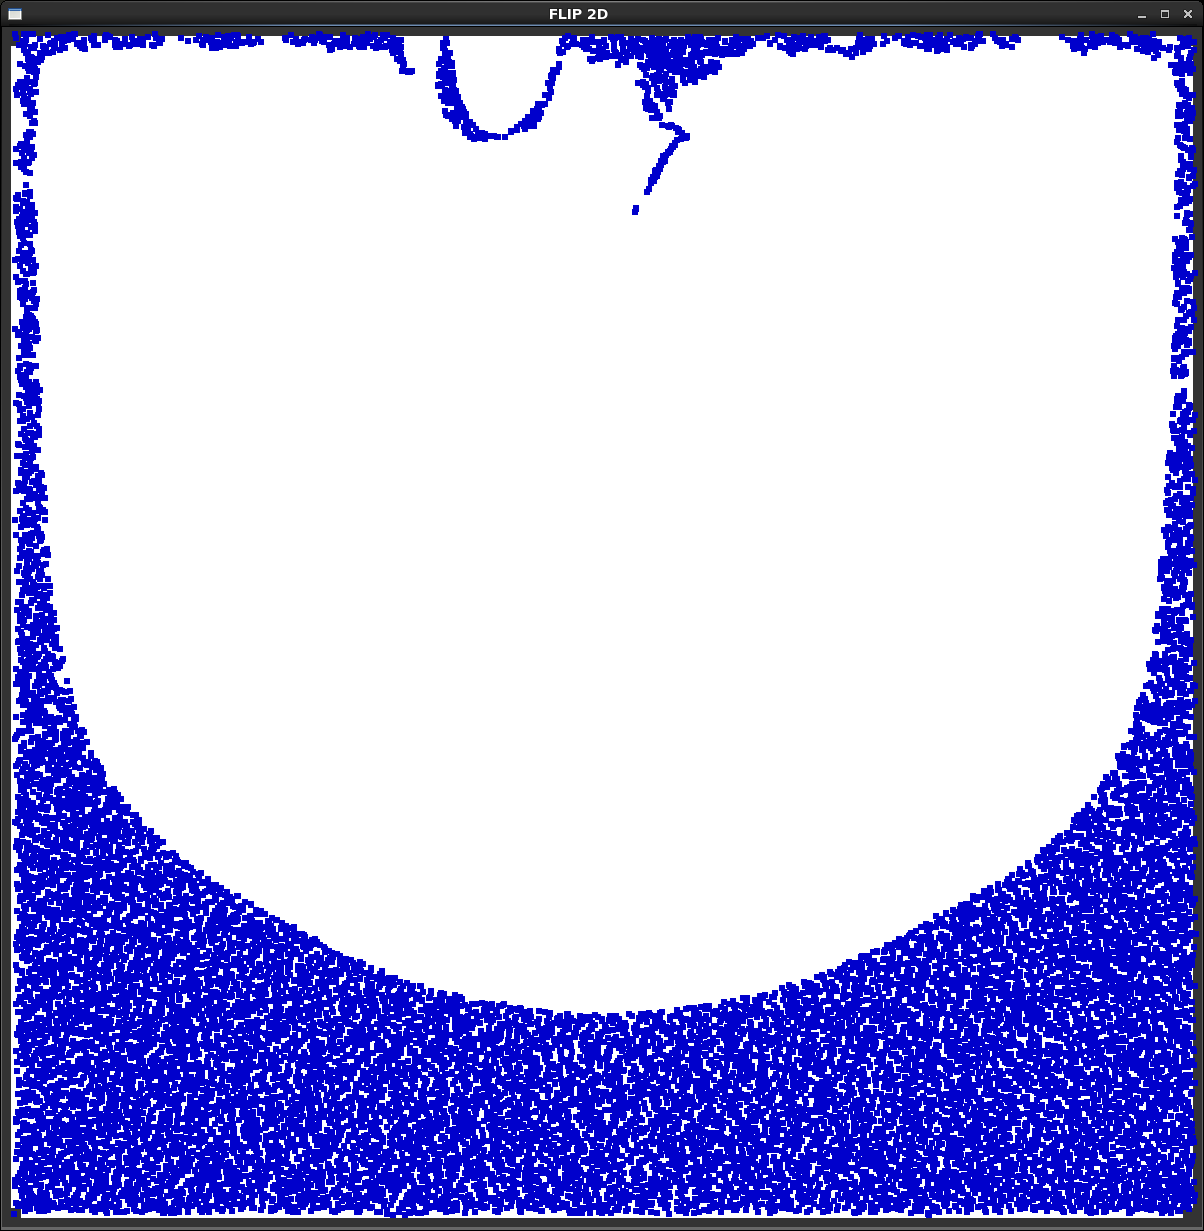
\includegraphics[height=35mm]{png/multigrid3.png}
\end{subfigure}
\begin{subfigure}[]{}
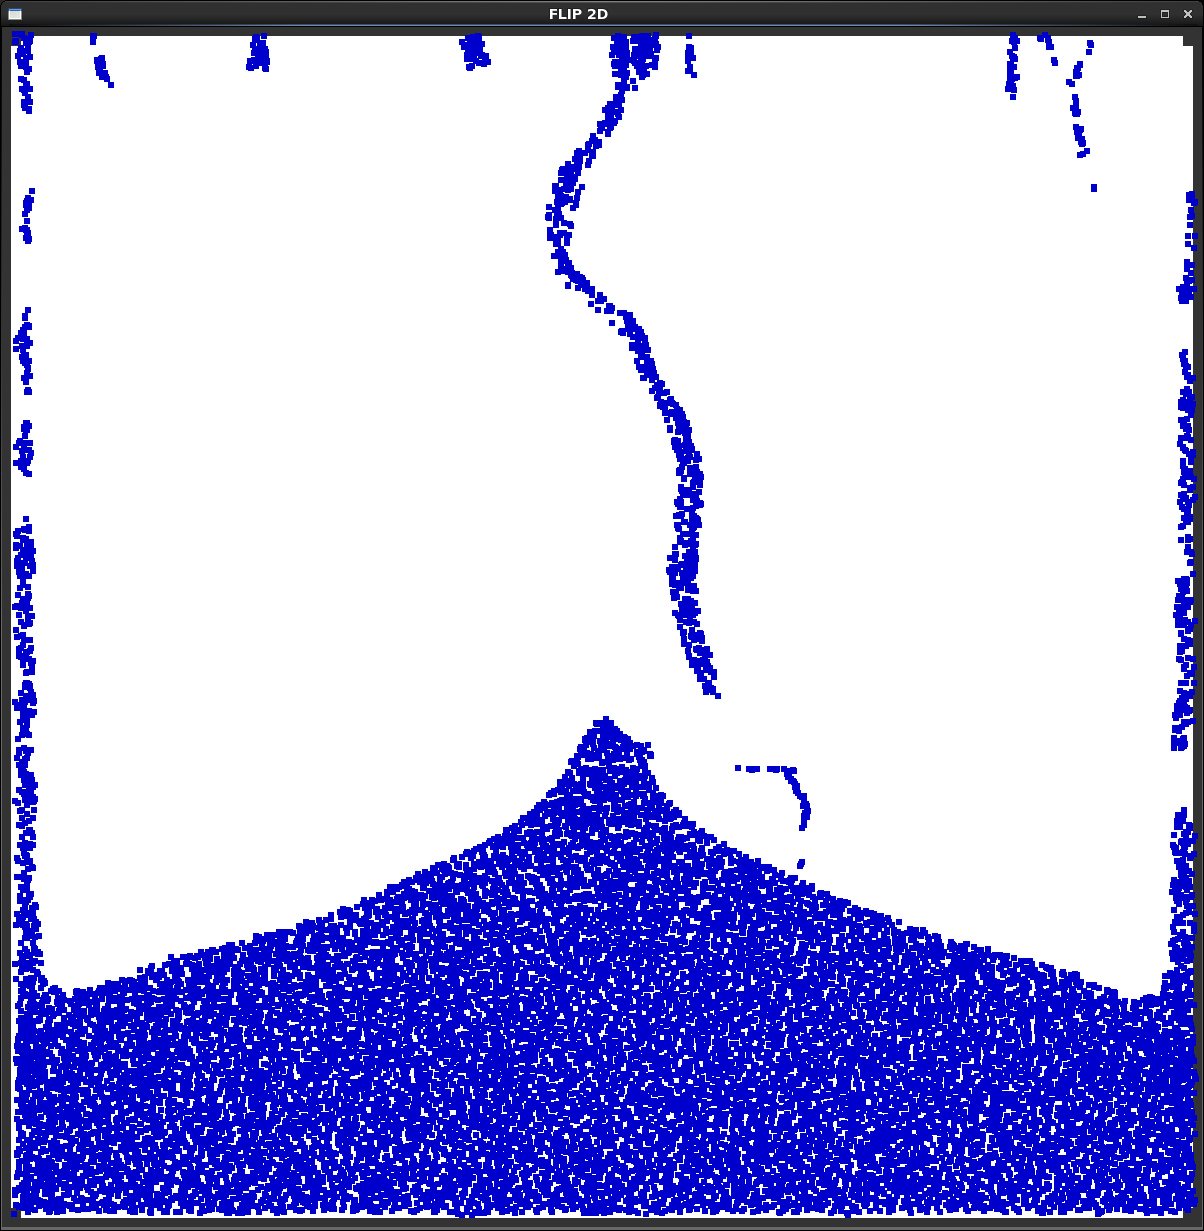
\includegraphics[height=35mm]{png/multigrid4.png}
\end{subfigure}
\begin{subfigure}[]{}
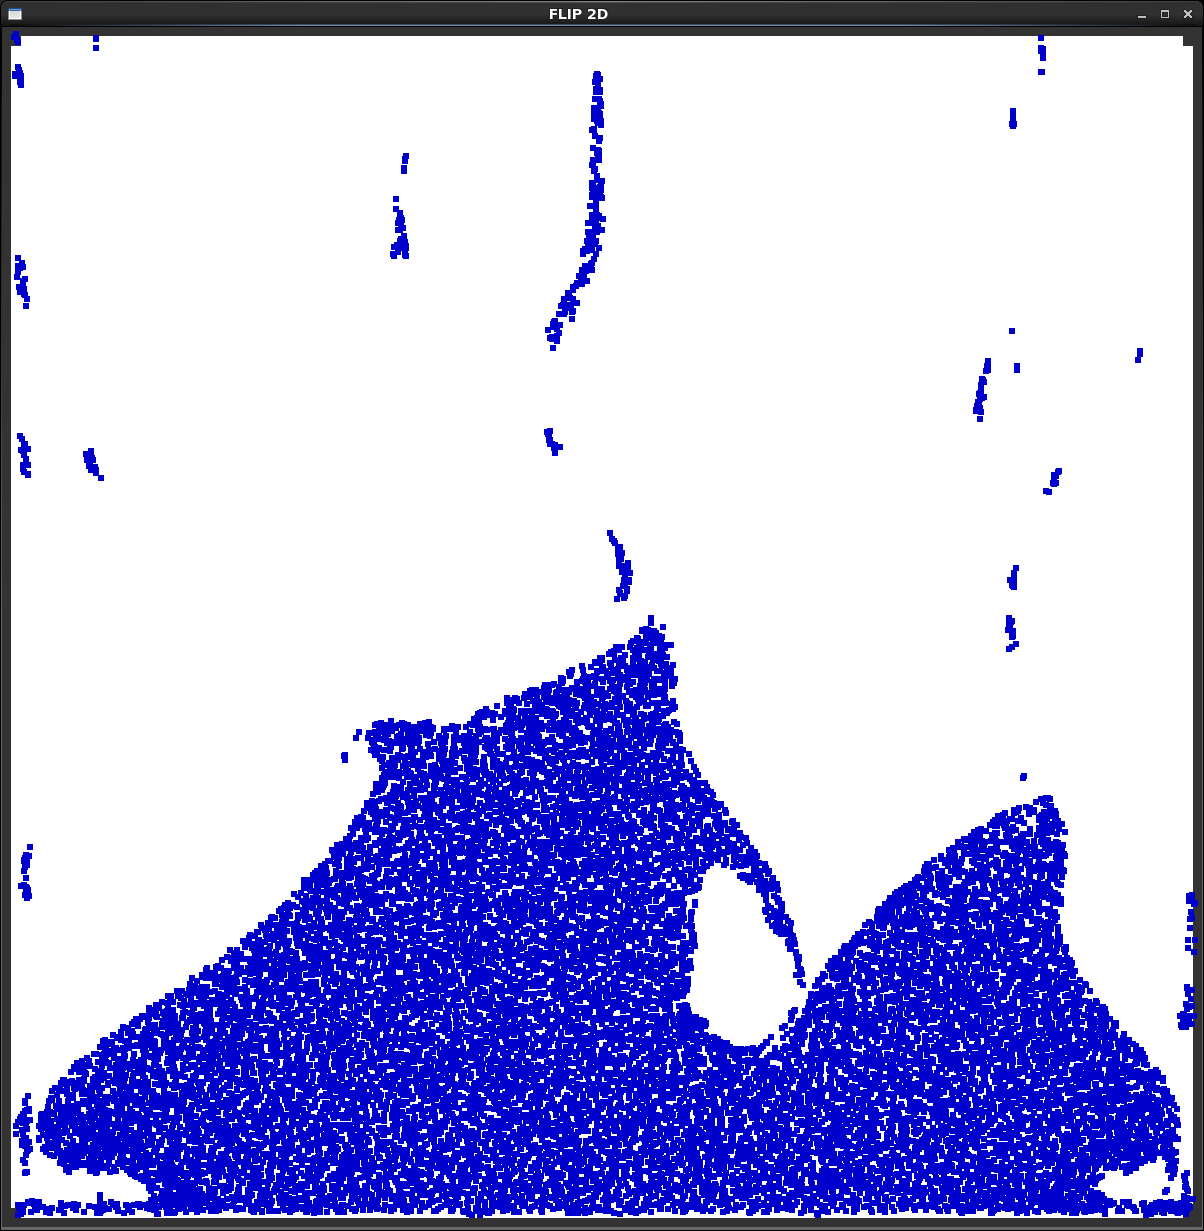
\includegraphics[height=35mm]{png/multigrid5.png}
\end{subfigure}
\begin{subfigure}[]{}
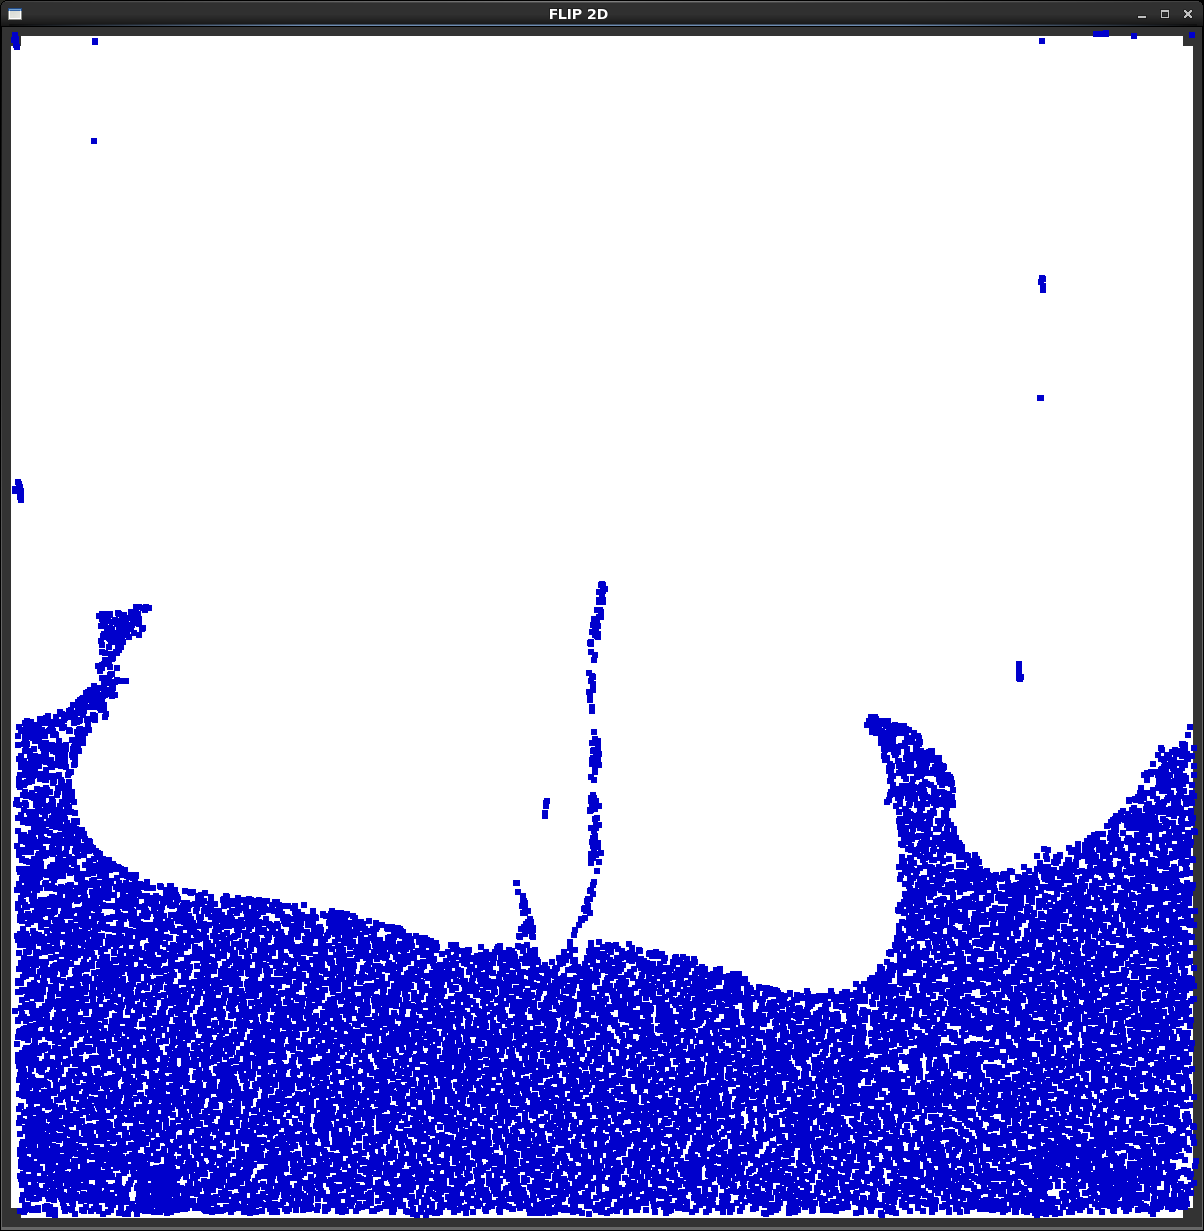
\includegraphics[height=35mm]{png/multigrid6.png}
\end{subfigure}
\begin{subfigure}[]{}
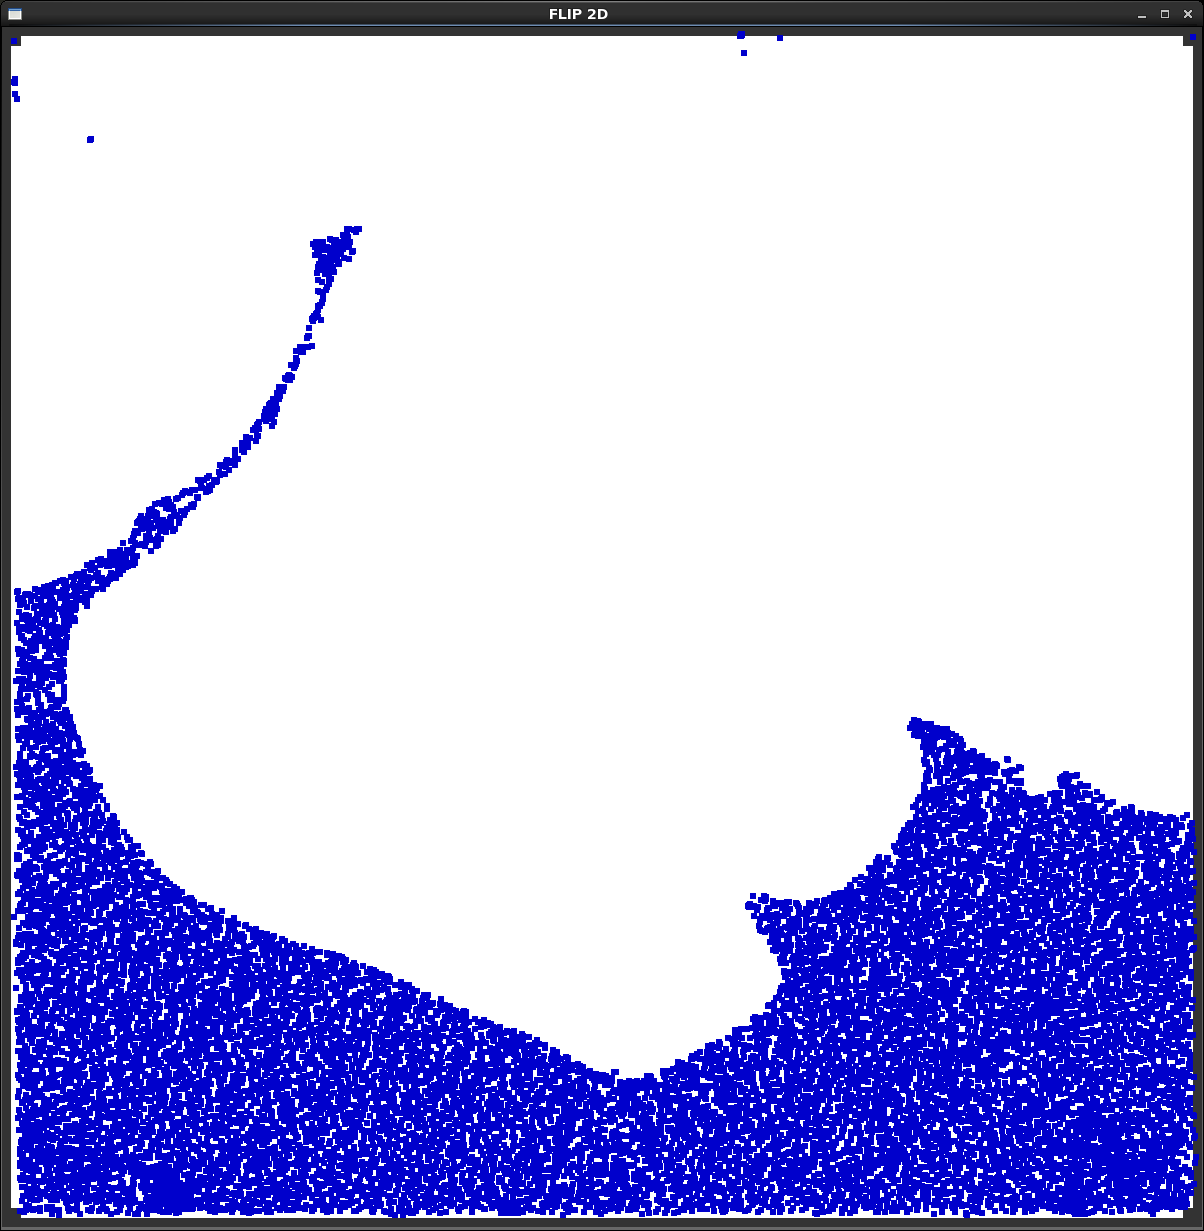
\includegraphics[height=35mm]{png/multigrid7.png}
\end{subfigure}
\begin{subfigure}[]{}
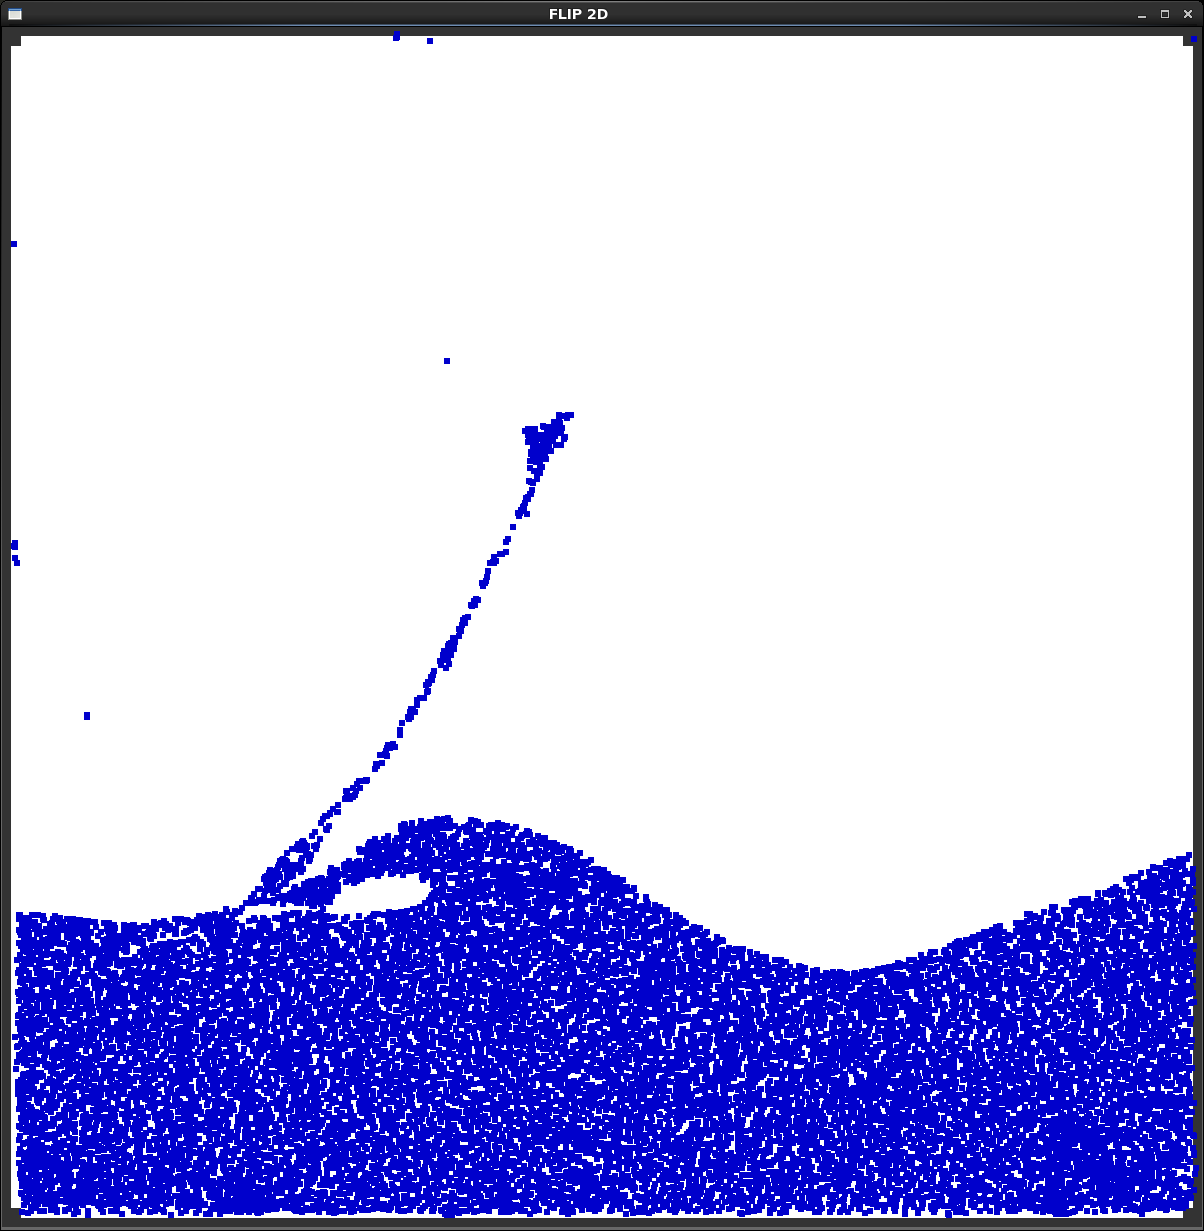
\includegraphics[height=35mm]{png/multigrid8.png}
\end{subfigure}
\begin{subfigure}[]{}
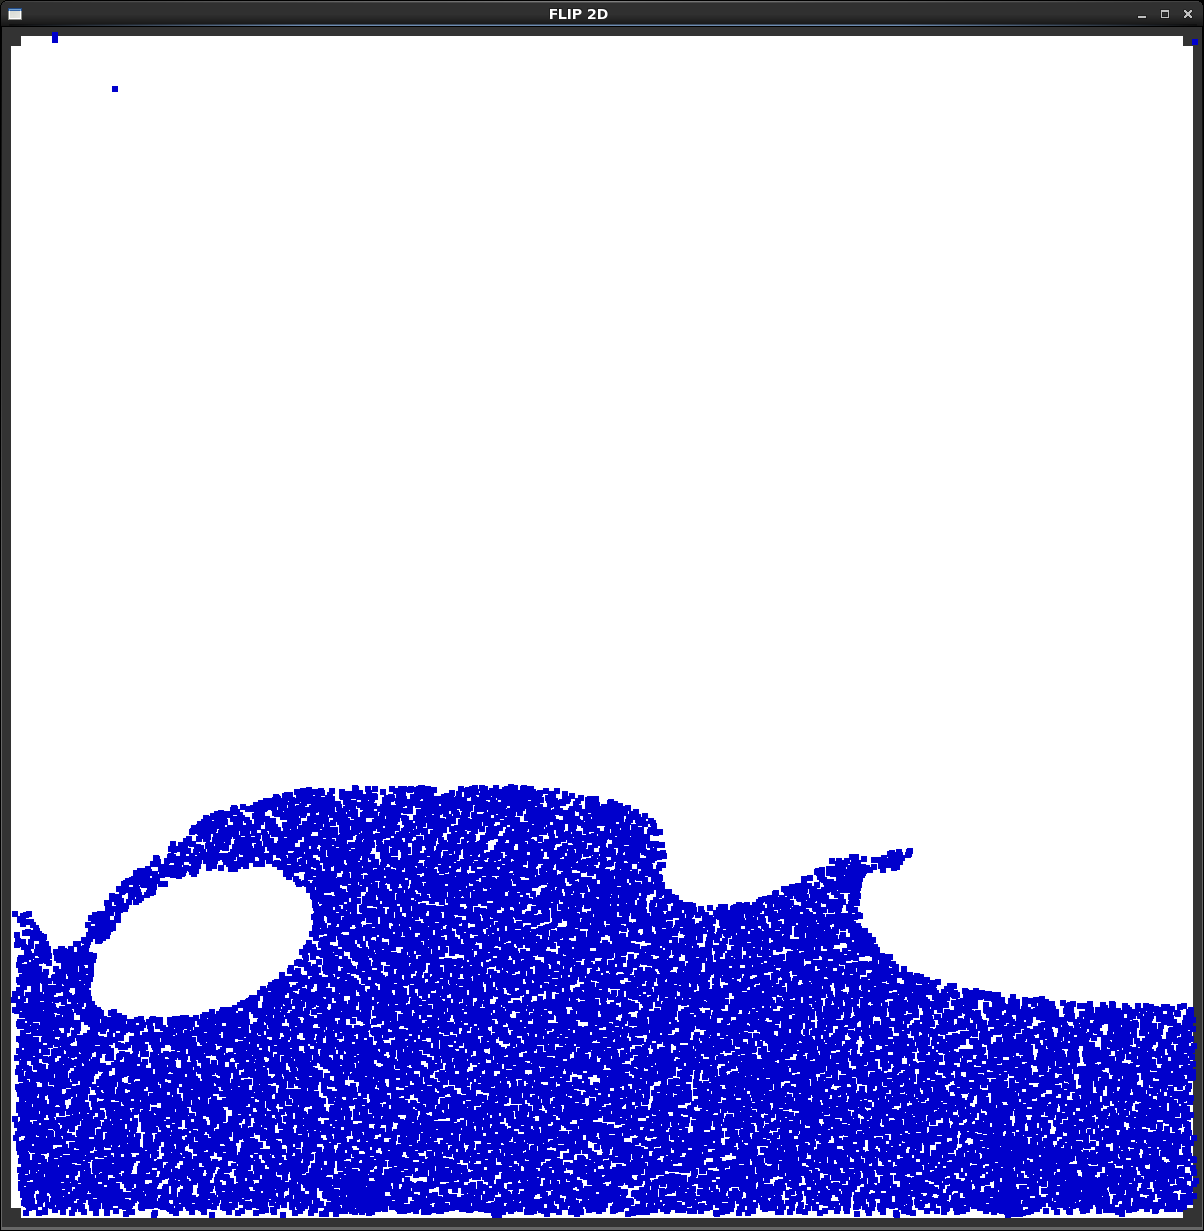
\includegraphics[height=35mm]{png/multigrid9.png}
\end{subfigure}
\begin{subfigure}[]{}
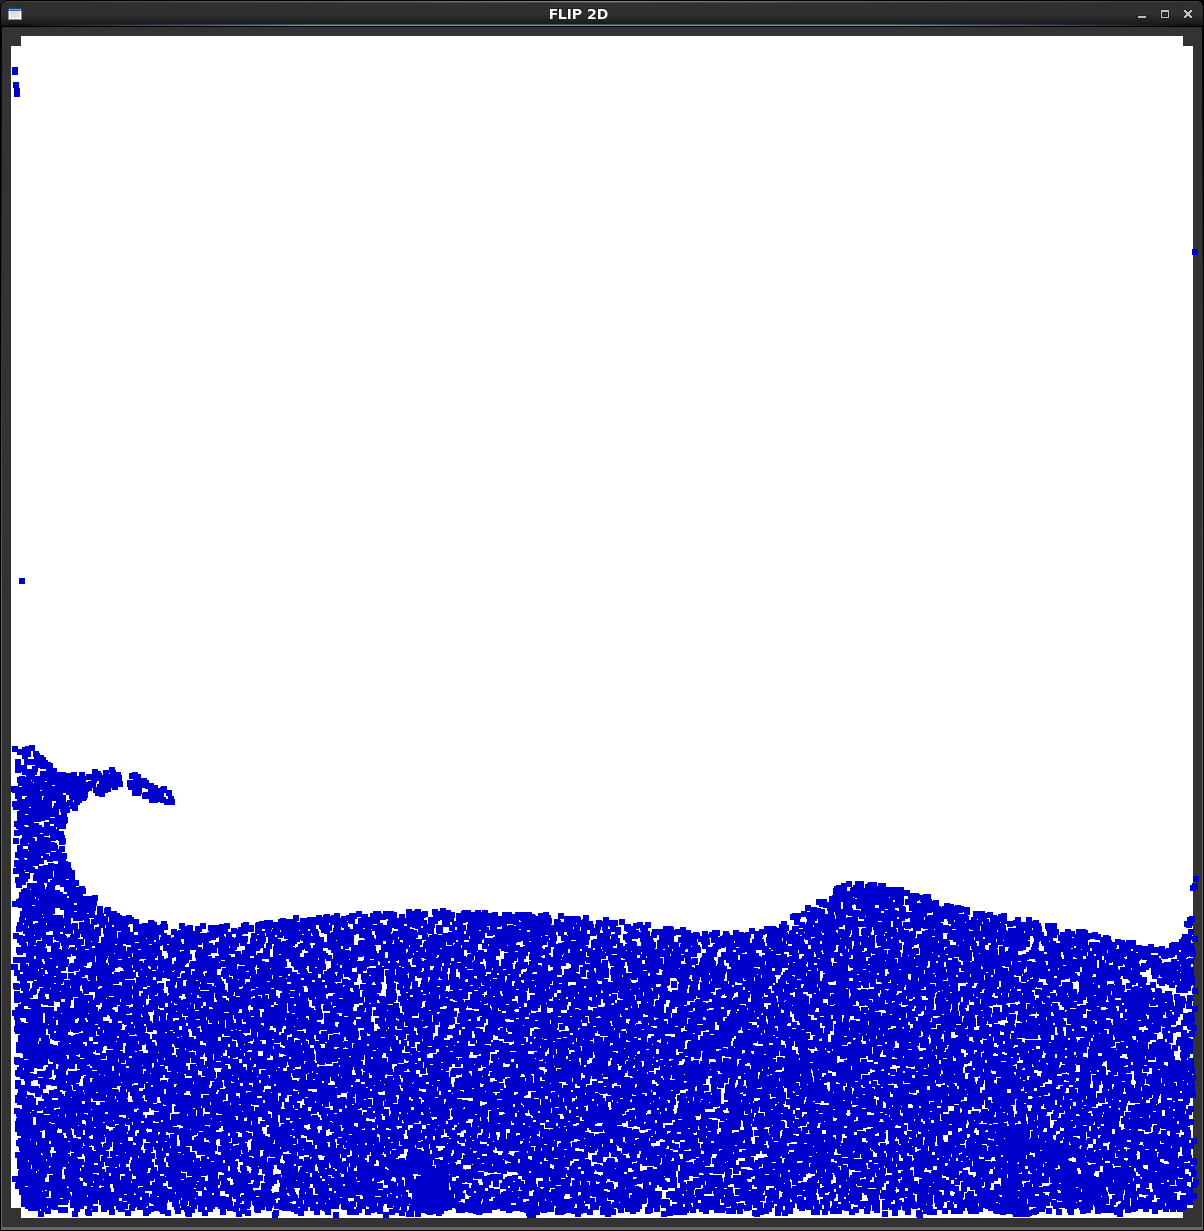
\includegraphics[height=35mm]{png/multigrid10.png}
\end{subfigure}
\begin{subfigure}[]{}
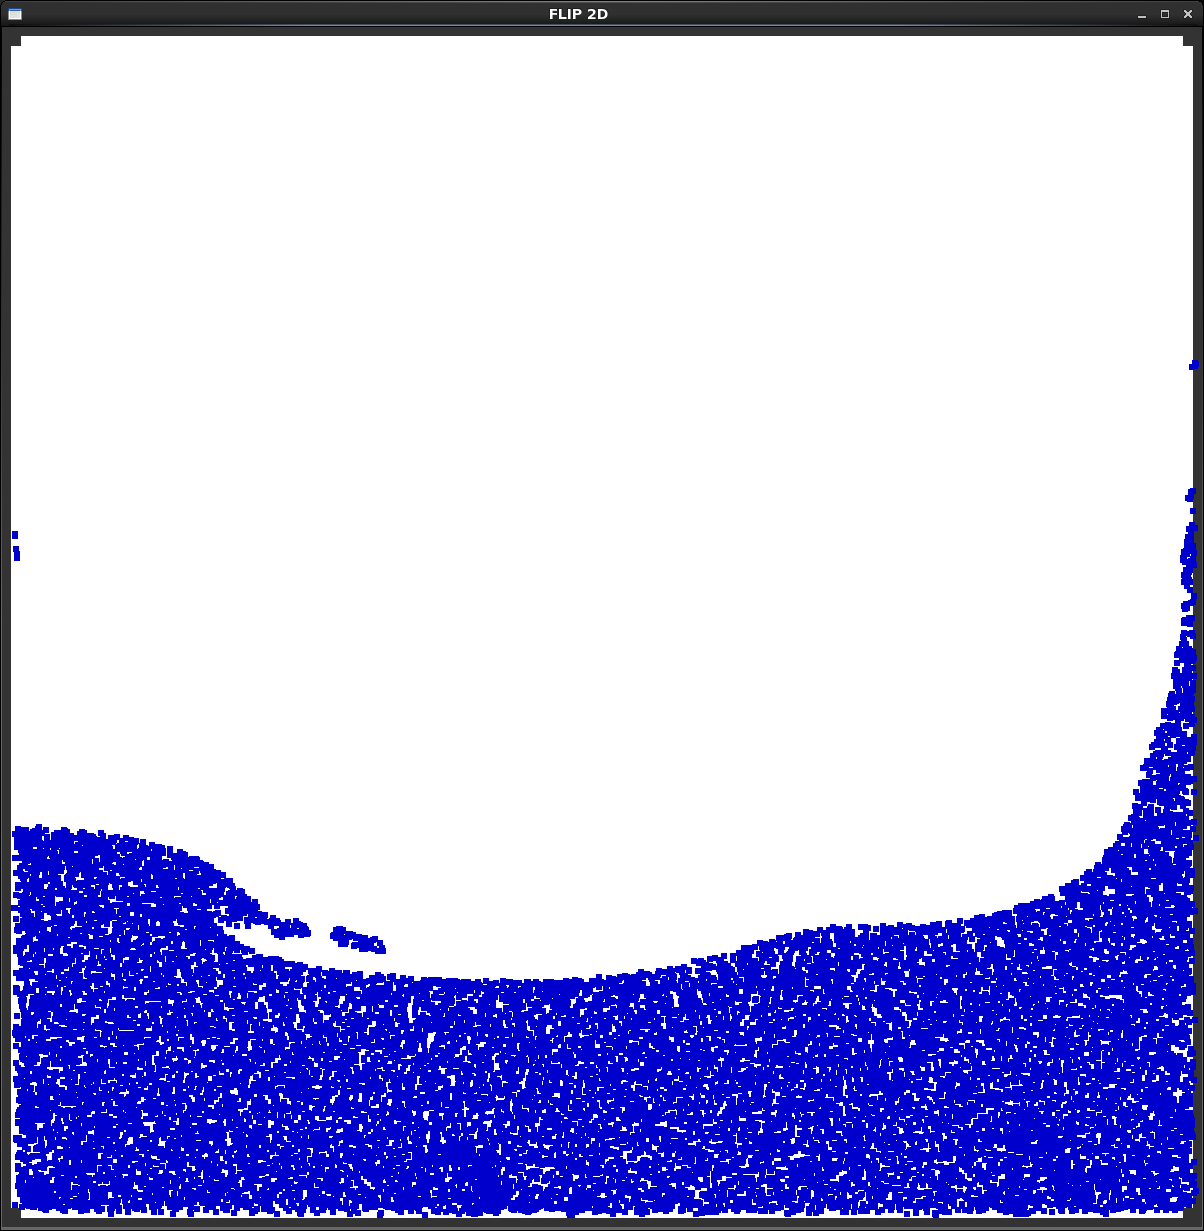
\includegraphics[height=35mm]{png/multigrid11.png}
\end{subfigure}
\caption{}
\label{multigrid}
\end{figure}

\newpage

\section*{Appendix B: Preconditioned Conjugate Gradient Simulation}
\addcontentsline{toc}{section}{Appendix B: Preconditioned Conjugate Gradient Simulation}
\begin{figure}[ht!]
\centering
\begin{subfigure}[]{}
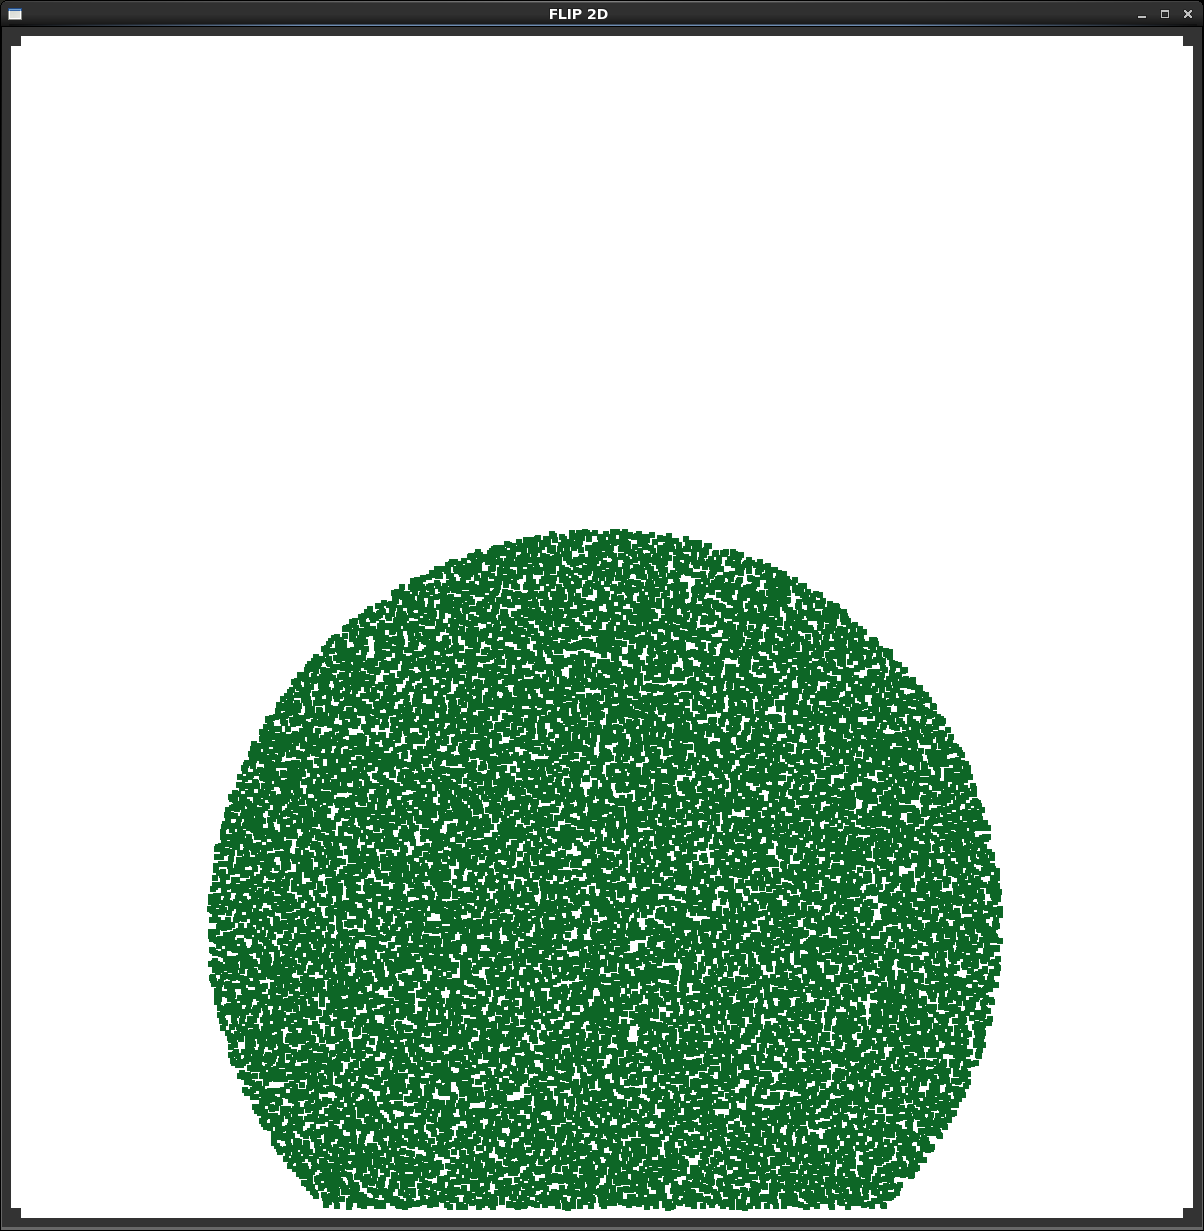
\includegraphics[height=35mm]{png/pcg0.png}
\end{subfigure}
\begin{subfigure}[]{}
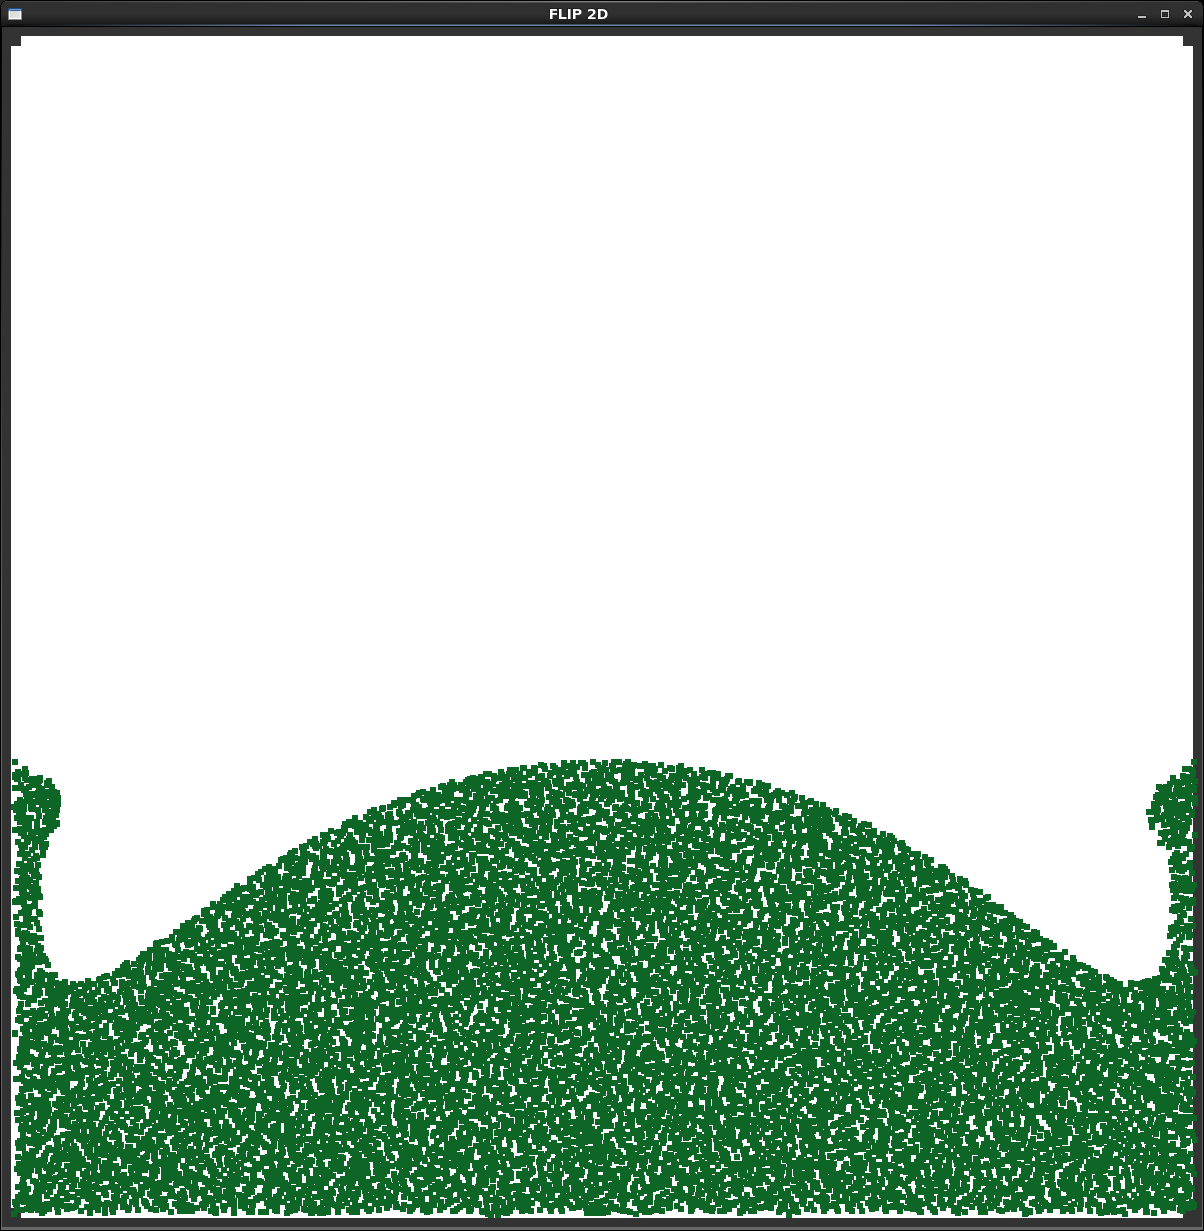
\includegraphics[height=35mm]{png/pcg1.png}
\end{subfigure}
\begin{subfigure}[]{}
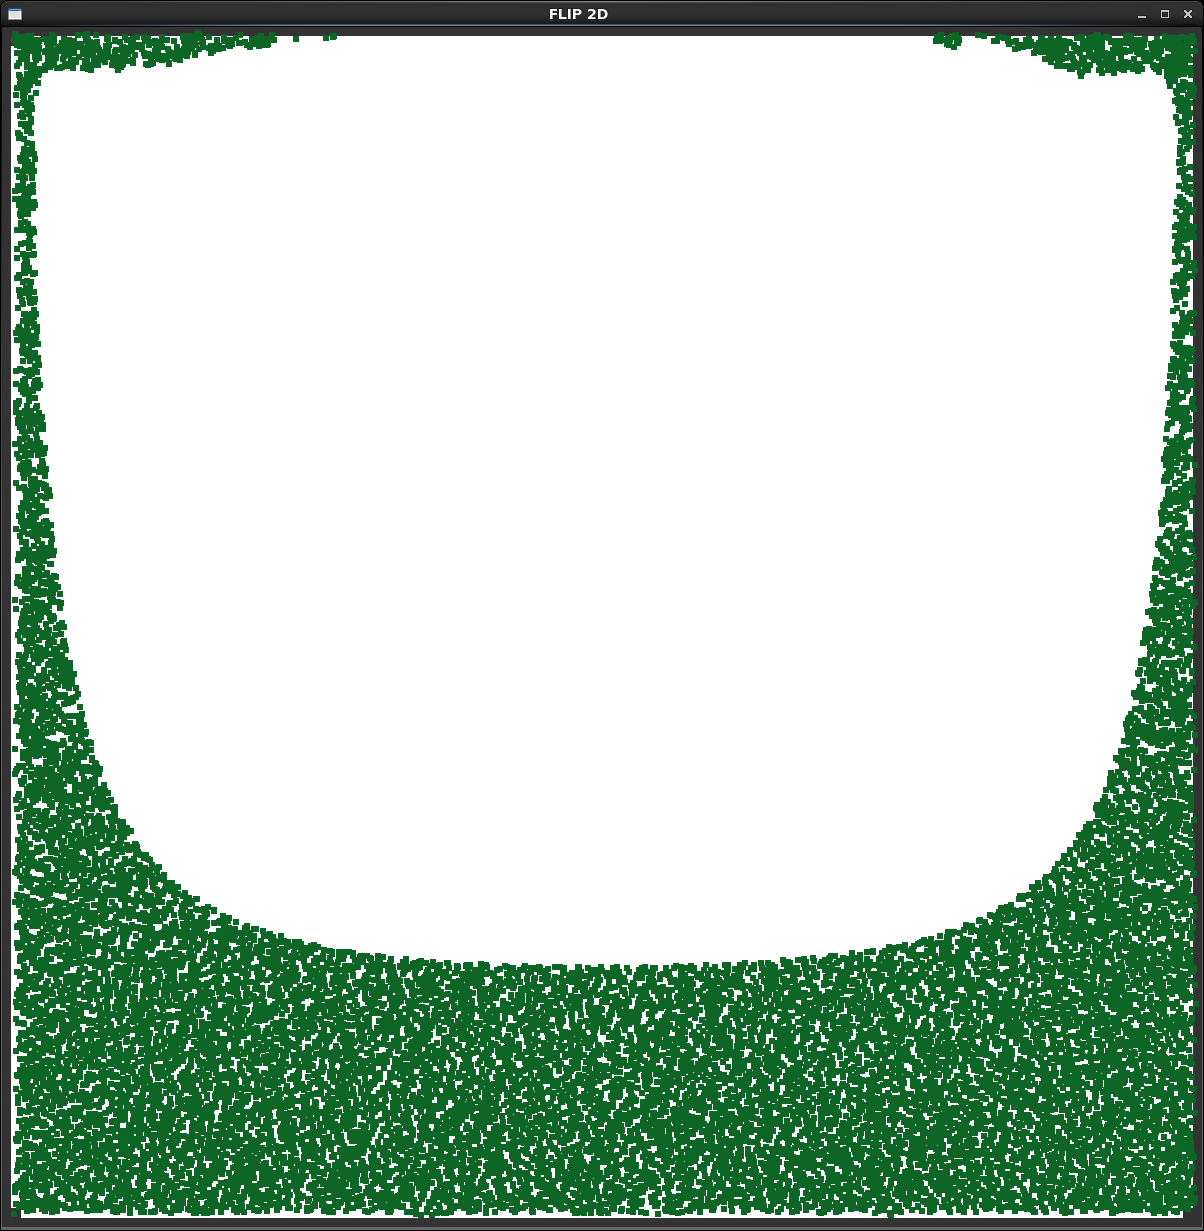
\includegraphics[height=35mm]{png/pcg2.png}
\end{subfigure}
\begin{subfigure}[]{}
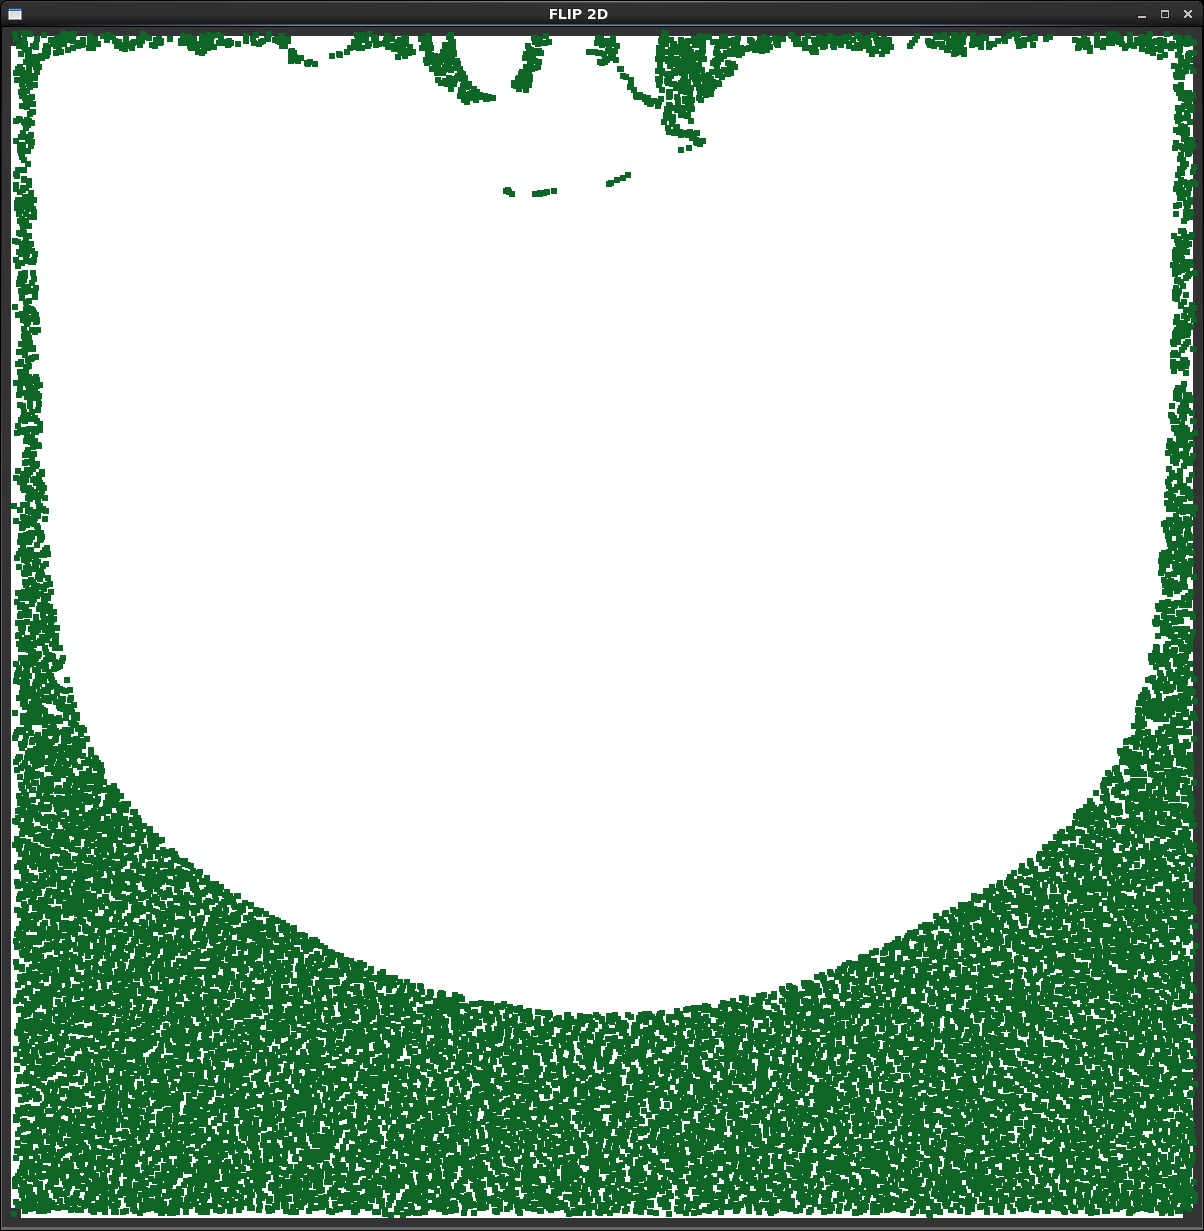
\includegraphics[height=35mm]{png/pcg3.png}
\end{subfigure}
\begin{subfigure}[]{}
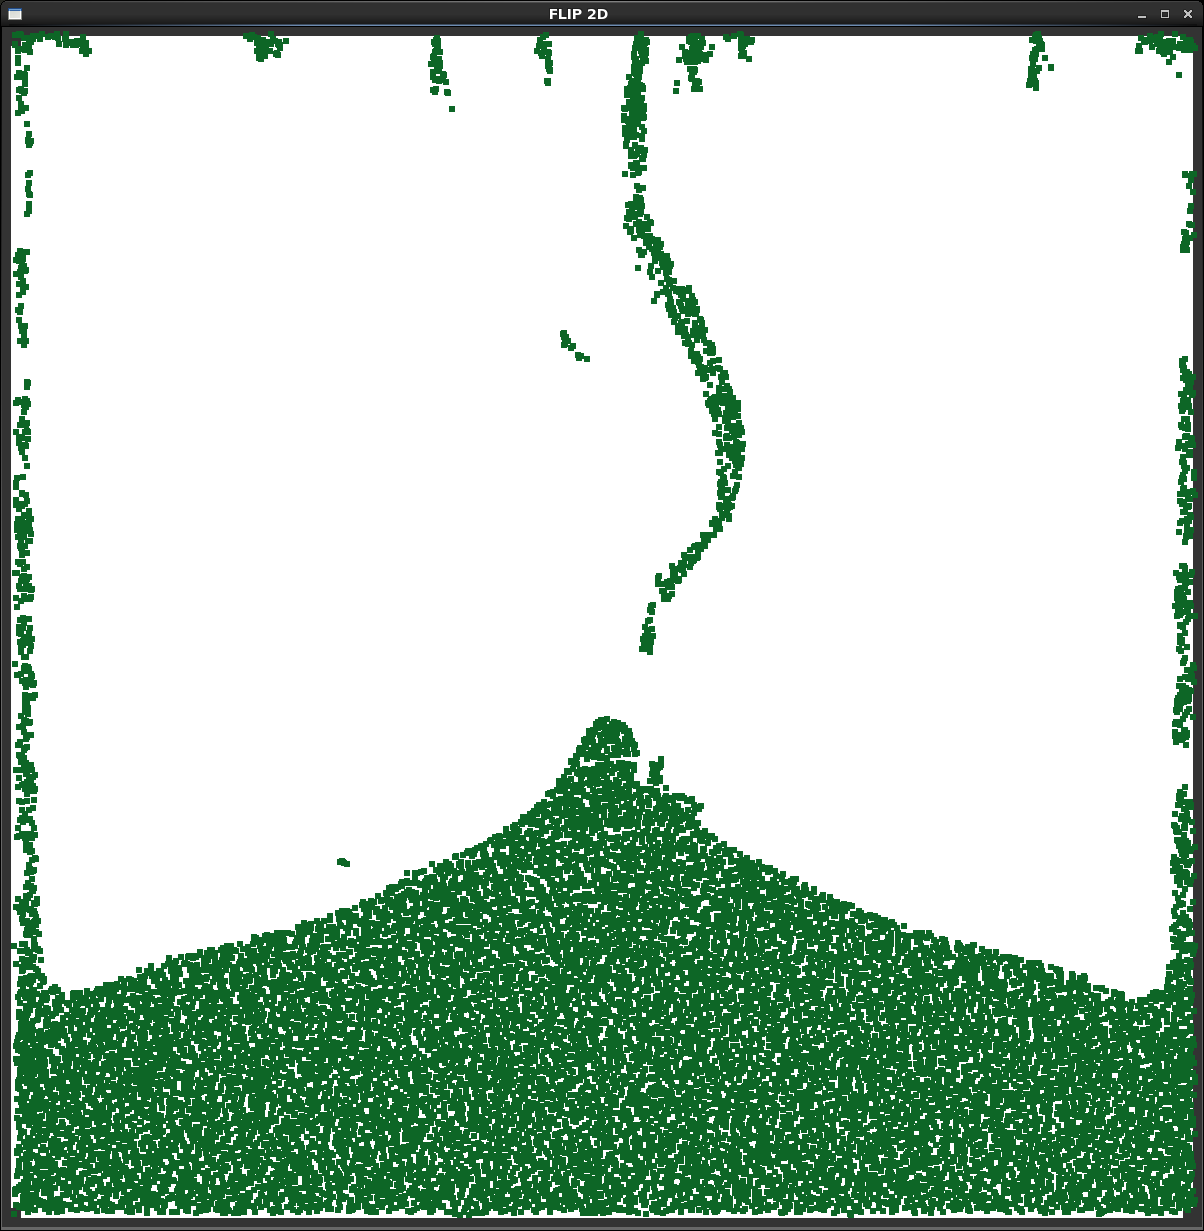
\includegraphics[height=35mm]{png/pcg4.png}
\end{subfigure}
\begin{subfigure}[]{}
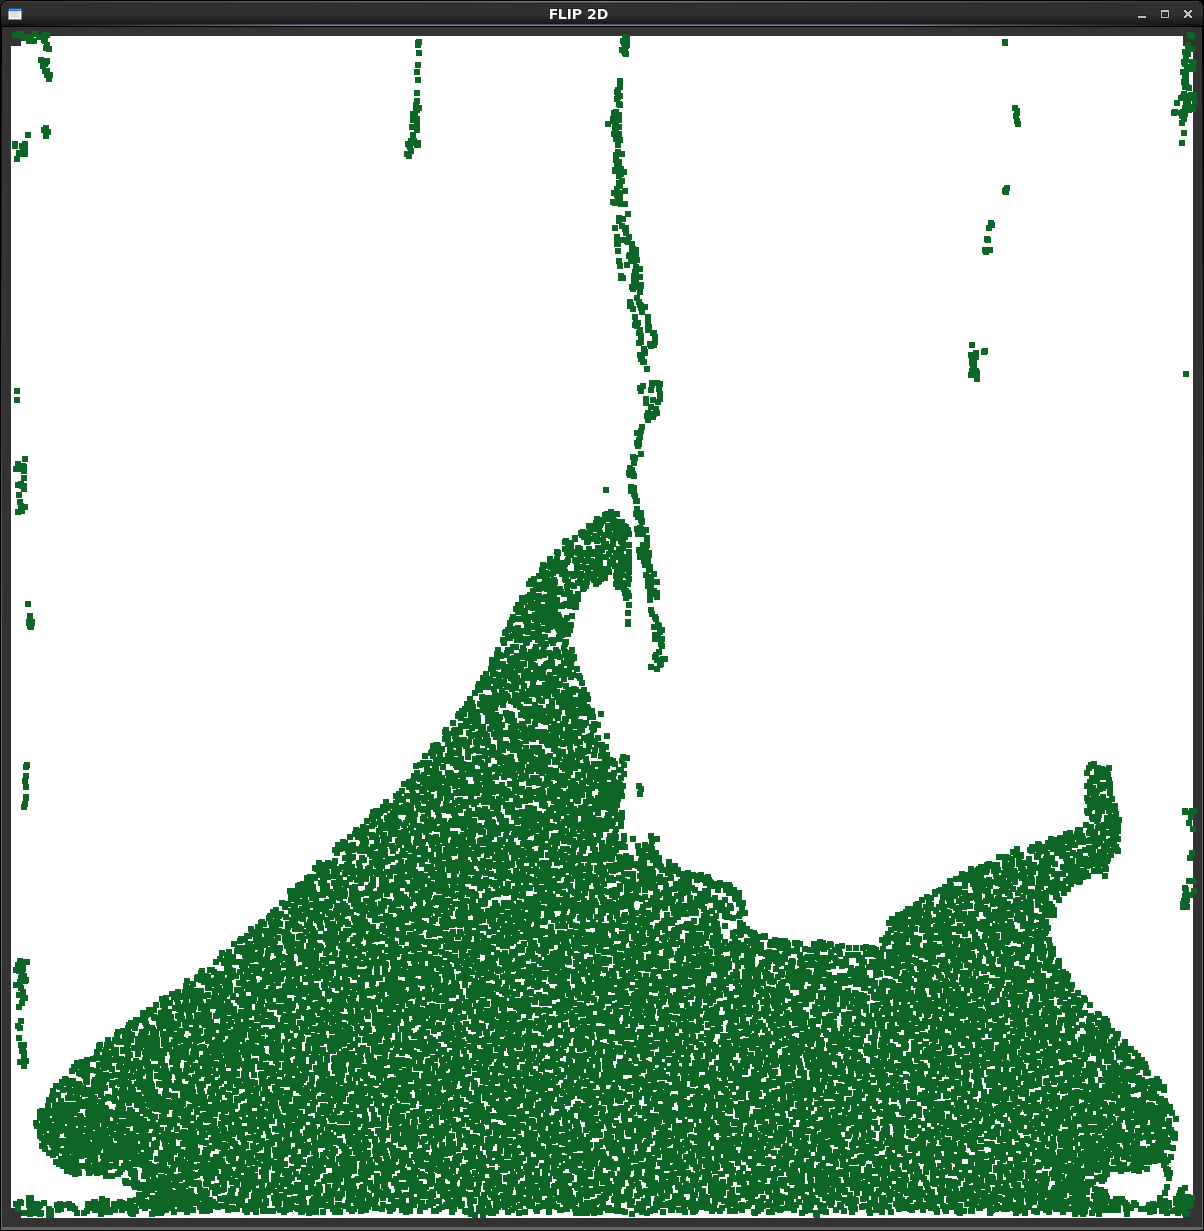
\includegraphics[height=35mm]{png/pcg5.png}
\end{subfigure}
\begin{subfigure}[]{}
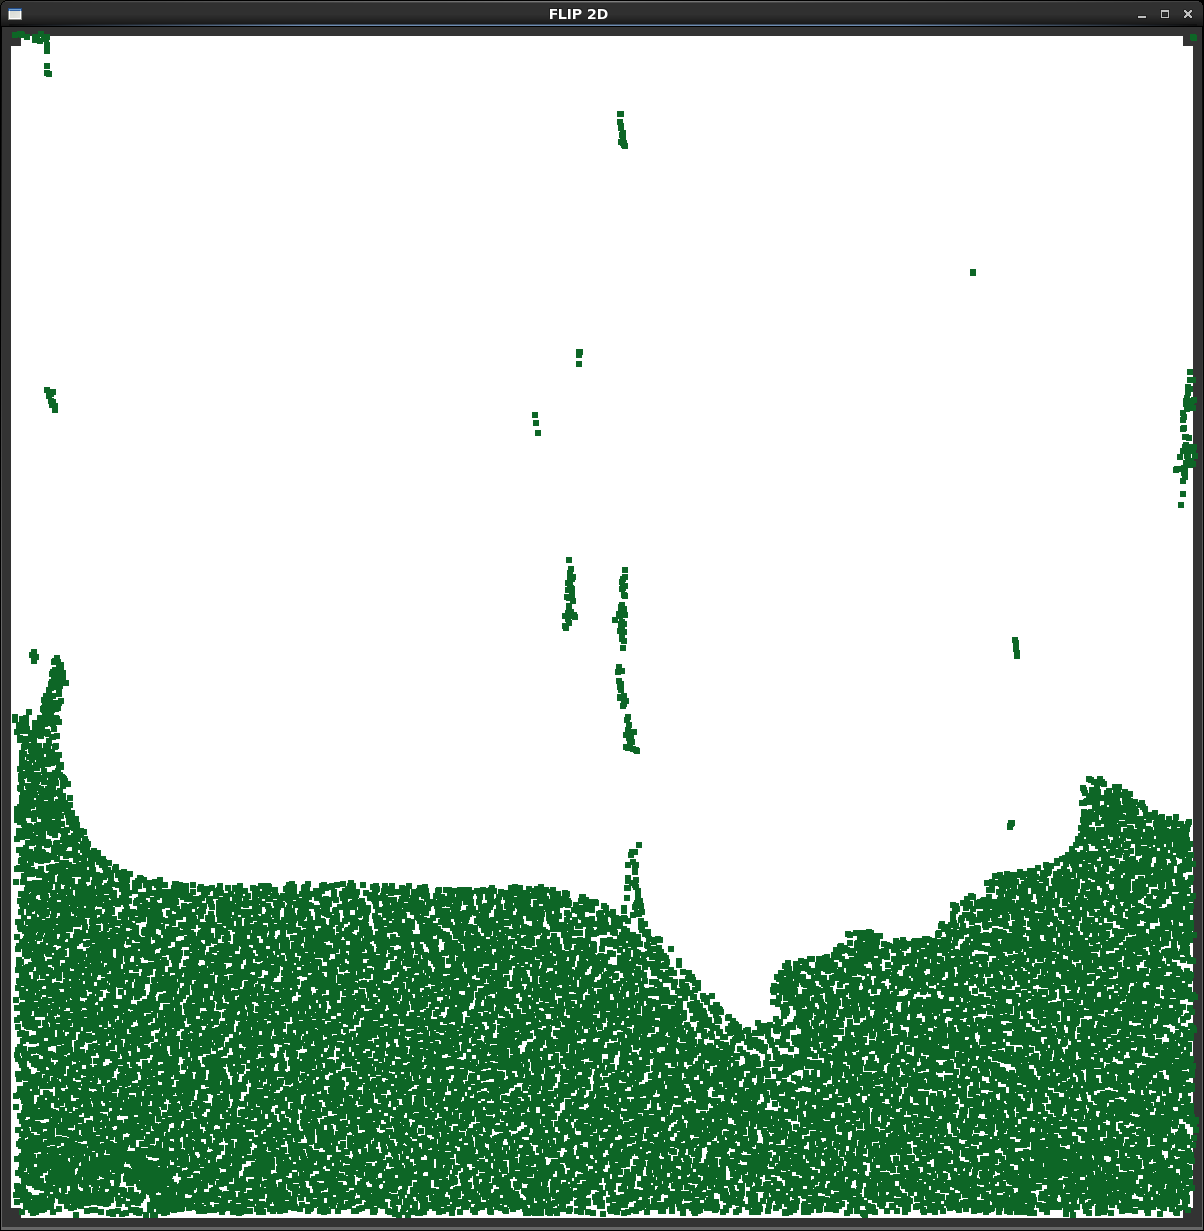
\includegraphics[height=35mm]{png/pcg6.png}
\end{subfigure}
\begin{subfigure}[]{}
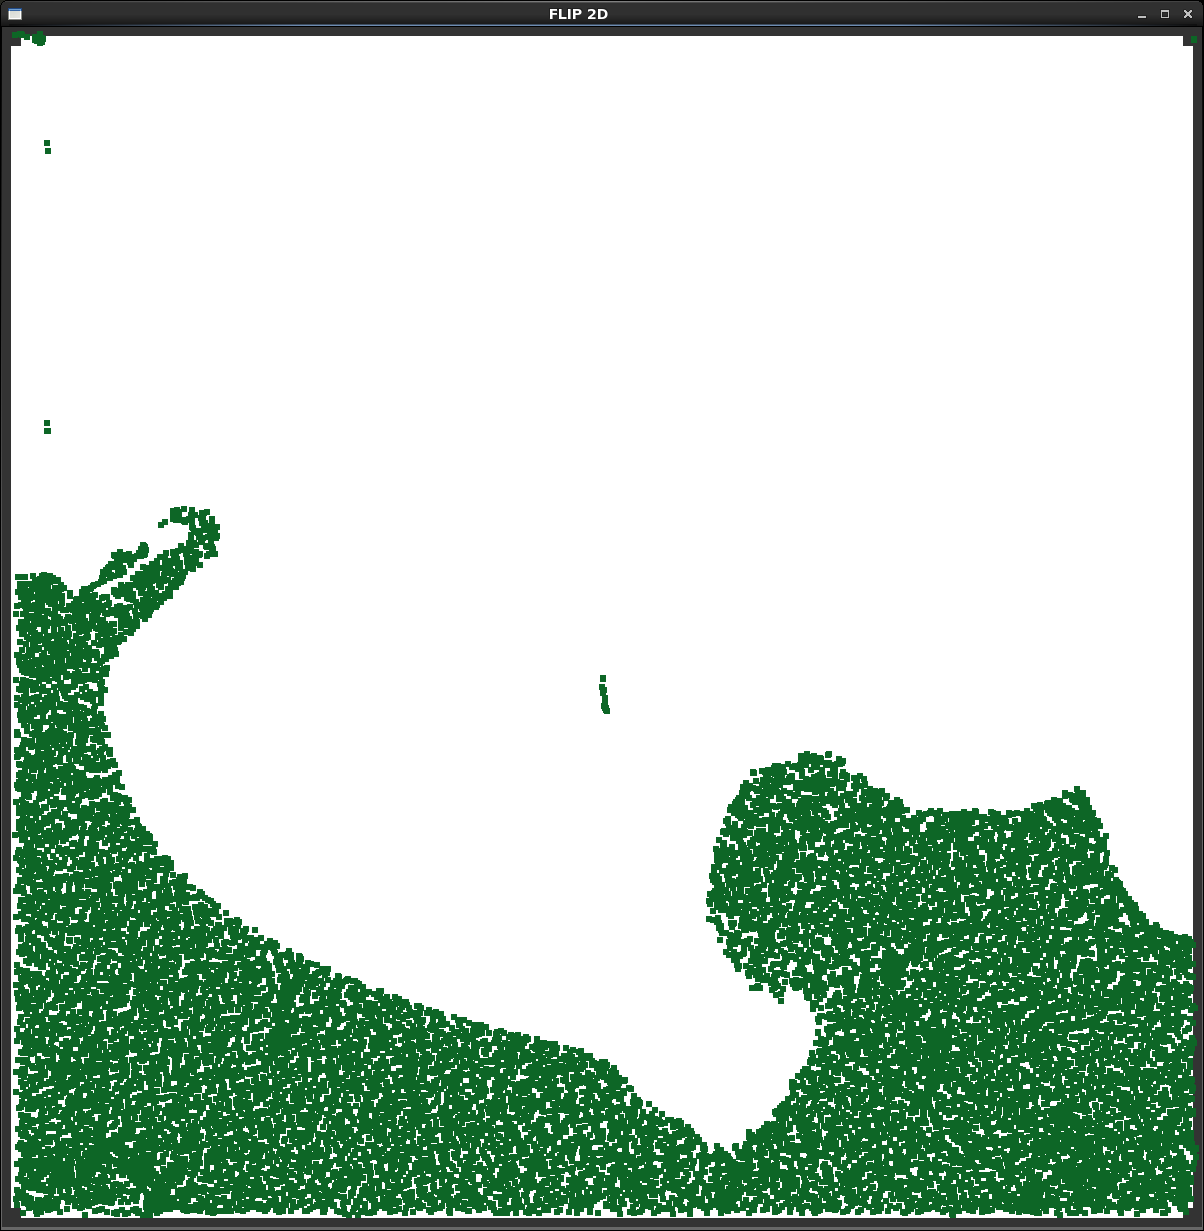
\includegraphics[height=35mm]{png/pcg7.png}
\end{subfigure}
\begin{subfigure}[]{}
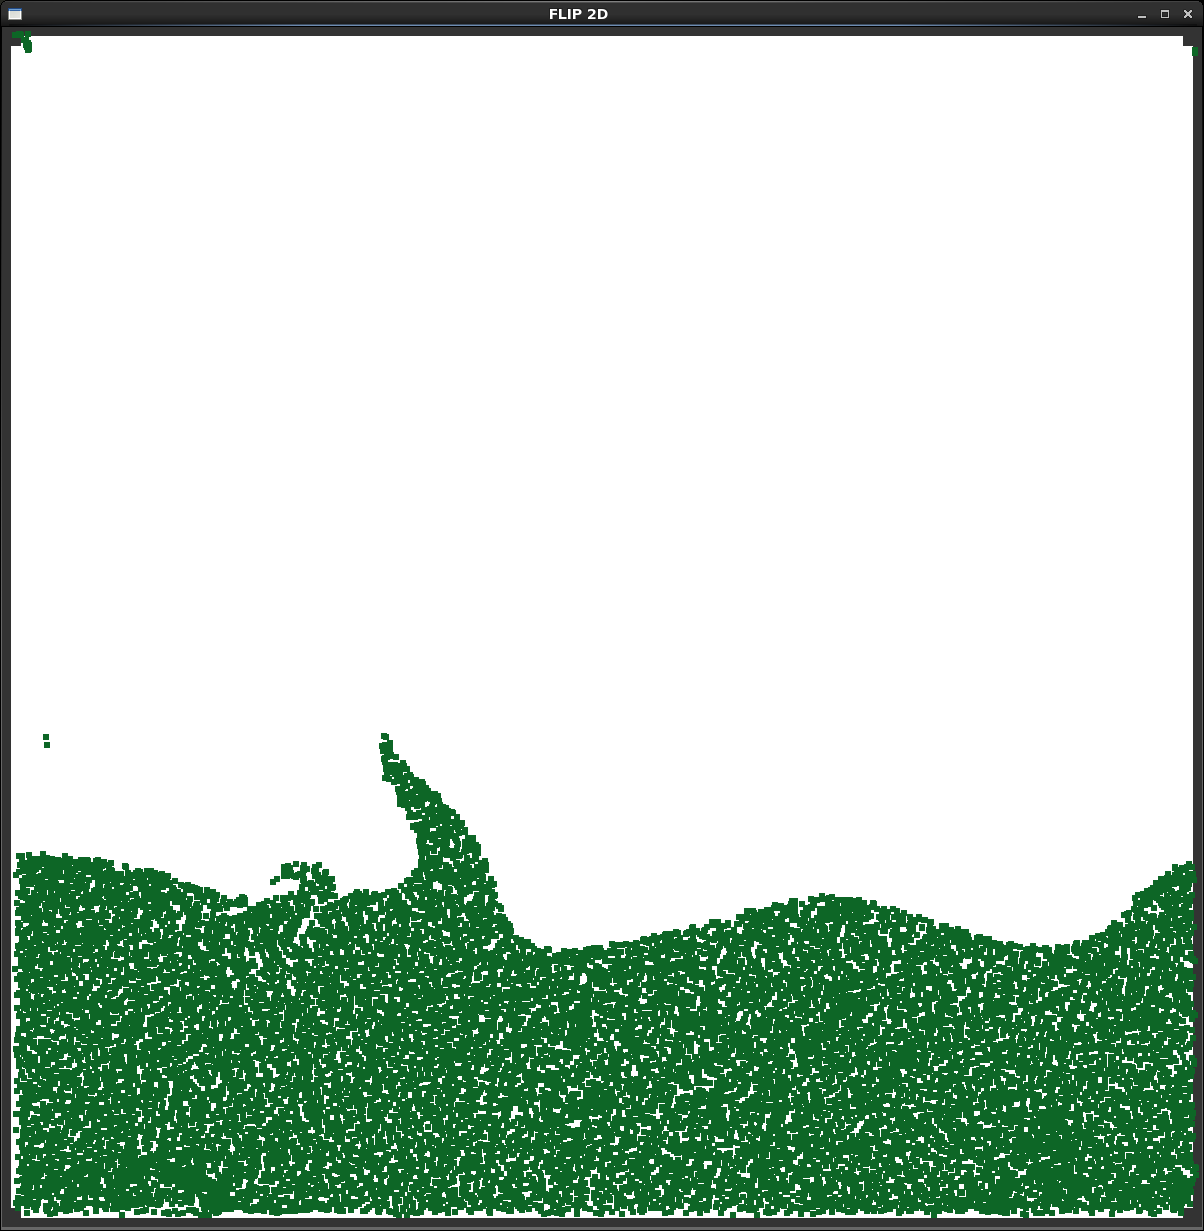
\includegraphics[height=35mm]{png/pcg8.png}
\end{subfigure}
\begin{subfigure}[]{}
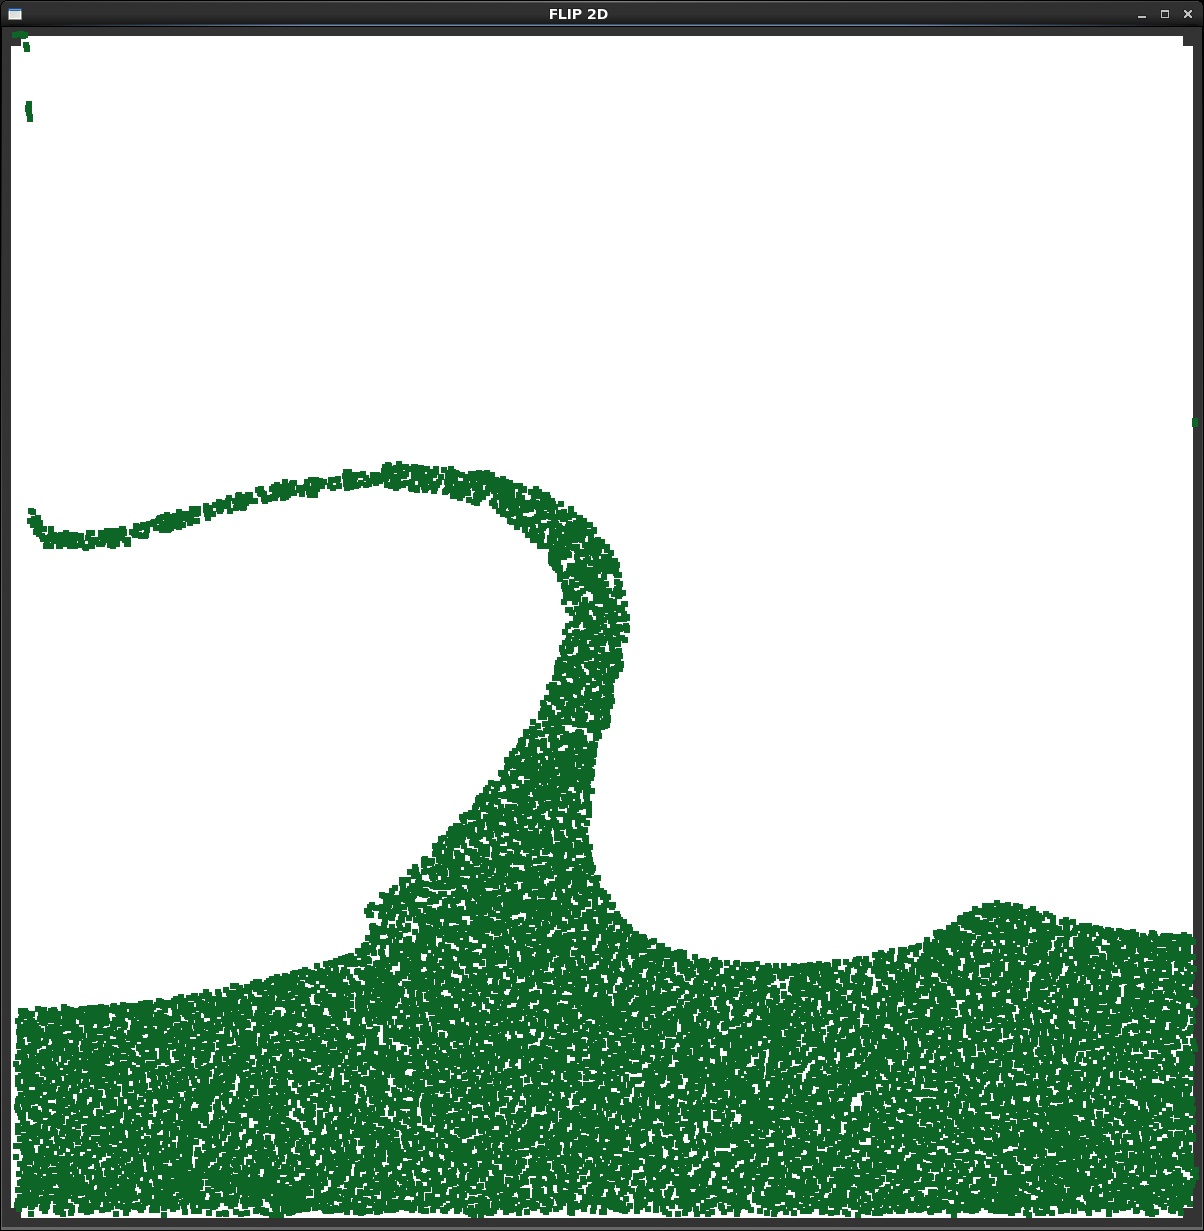
\includegraphics[height=35mm]{png/pcg9.png}
\end{subfigure}
\begin{subfigure}[]{}
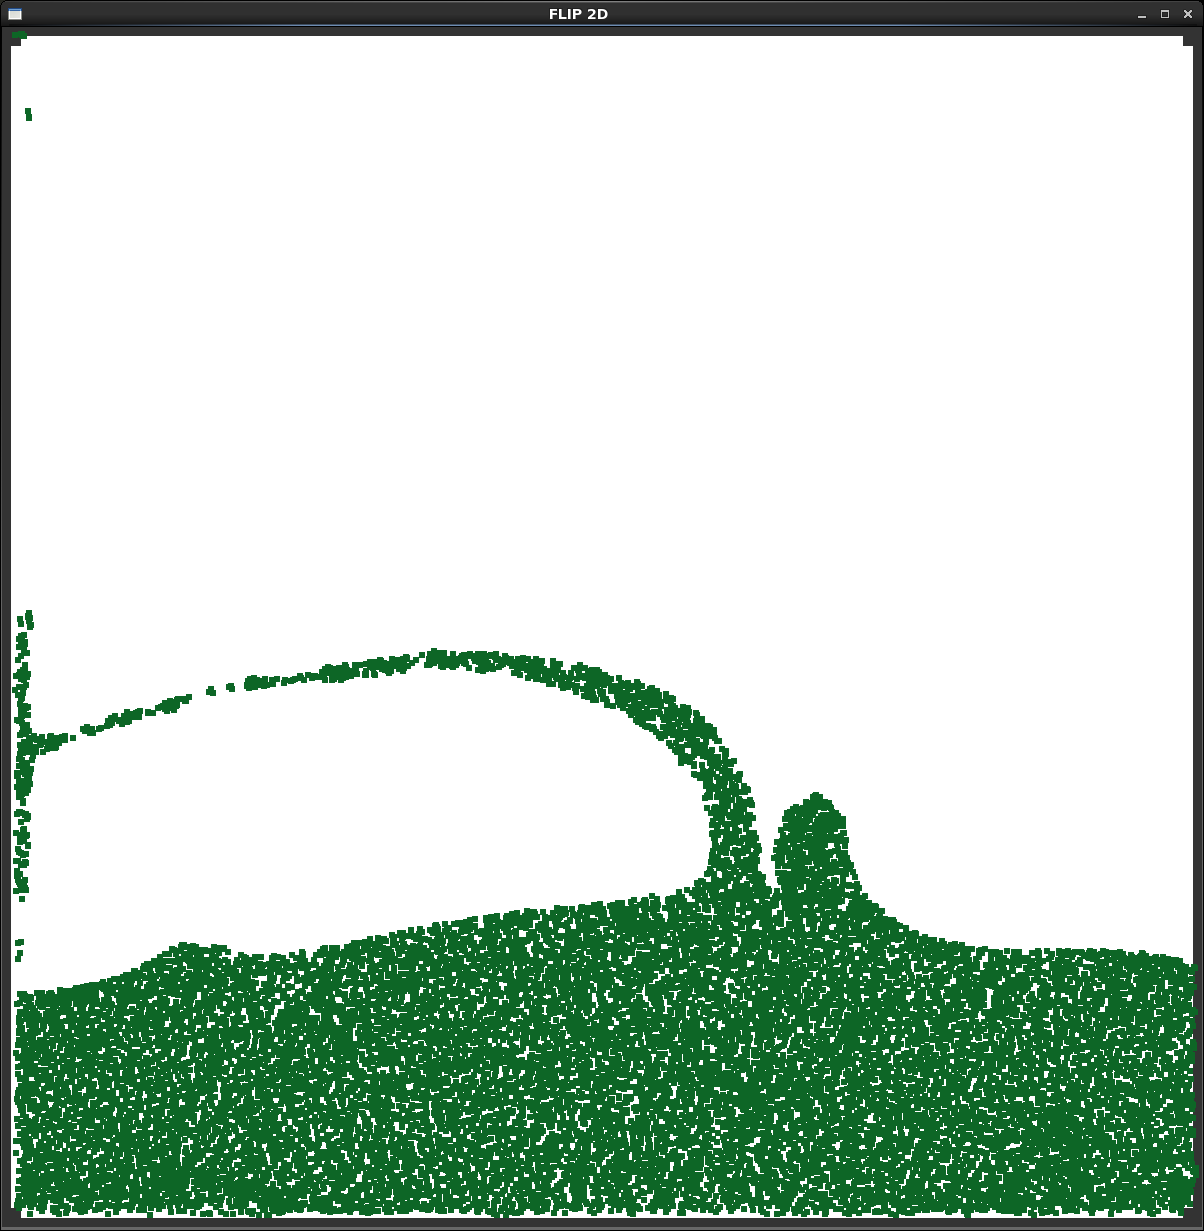
\includegraphics[height=35mm]{png/pcg10.png}
\end{subfigure}
\begin{subfigure}[]{}
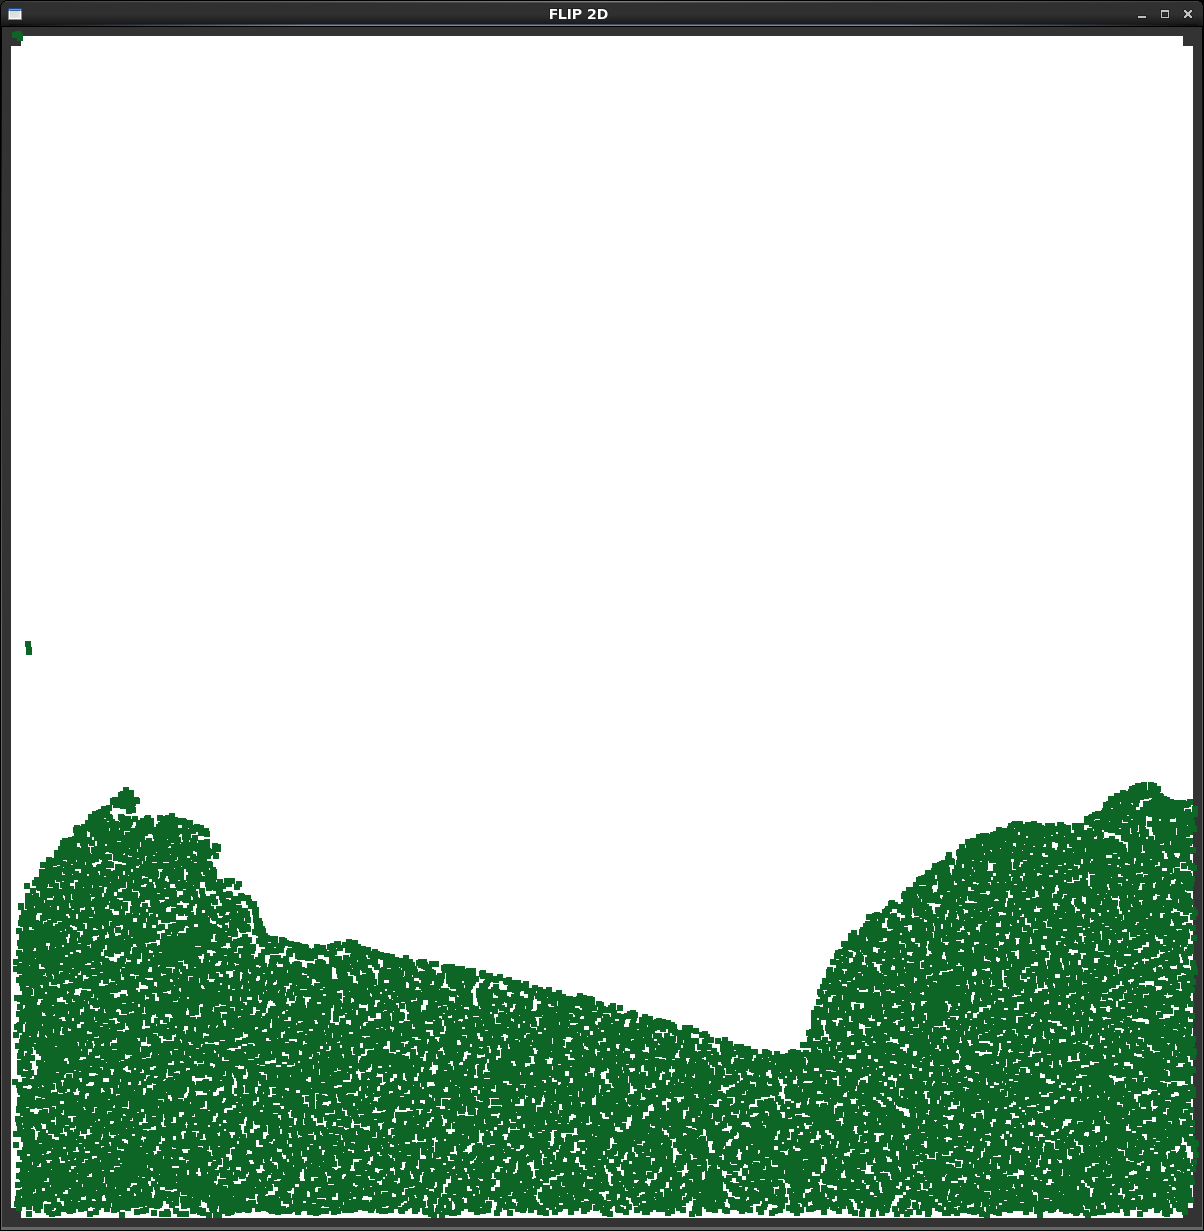
\includegraphics[height=35mm]{png/pcg11.png}
\end{subfigure}
\caption{}
\label{multigrid}
\end{figure}


\end{document}
